\documentclass[12pt]{scrreprt}
\usepackage{graphicx}
\usepackage{amsmath}
\usepackage{geometry}

\newcommand{\RN}[1]{%
  \textup{\uppercase\expandafter{\romannumeral#1}}%
}

\setlength{\parindent}{0pt}

\usepackage{fourier} 
\usepackage{array}
\usepackage{makecell}

%\renewcommand{\arraystretch}{1.5}
%\renewcommand{\cellalign/theadalign}{cl}

\begin{document}
\title{Interaction of a "cold plume" with a subduction zone}
\subtitle{Semester Thesis}
\author{Florian Frei}

\maketitle

\newpage

\tableofcontents

\newpage

\section{Motivation}
Seismological measurements from Columbia shown in figure \ref{fig:seism_data} suggests that an rare geological scenario is happening. The geophysical community agrees that what is probably happening is the rare case where a "cold plume" is detached from the lithosphere and interacts with the subduction plate beneath it. In this project the goal is to use a simplified subduction model to simulate what longterm tendencies could develop and investigate the sensitivity on the parameters for the individual scenarios.
\begin{figure}
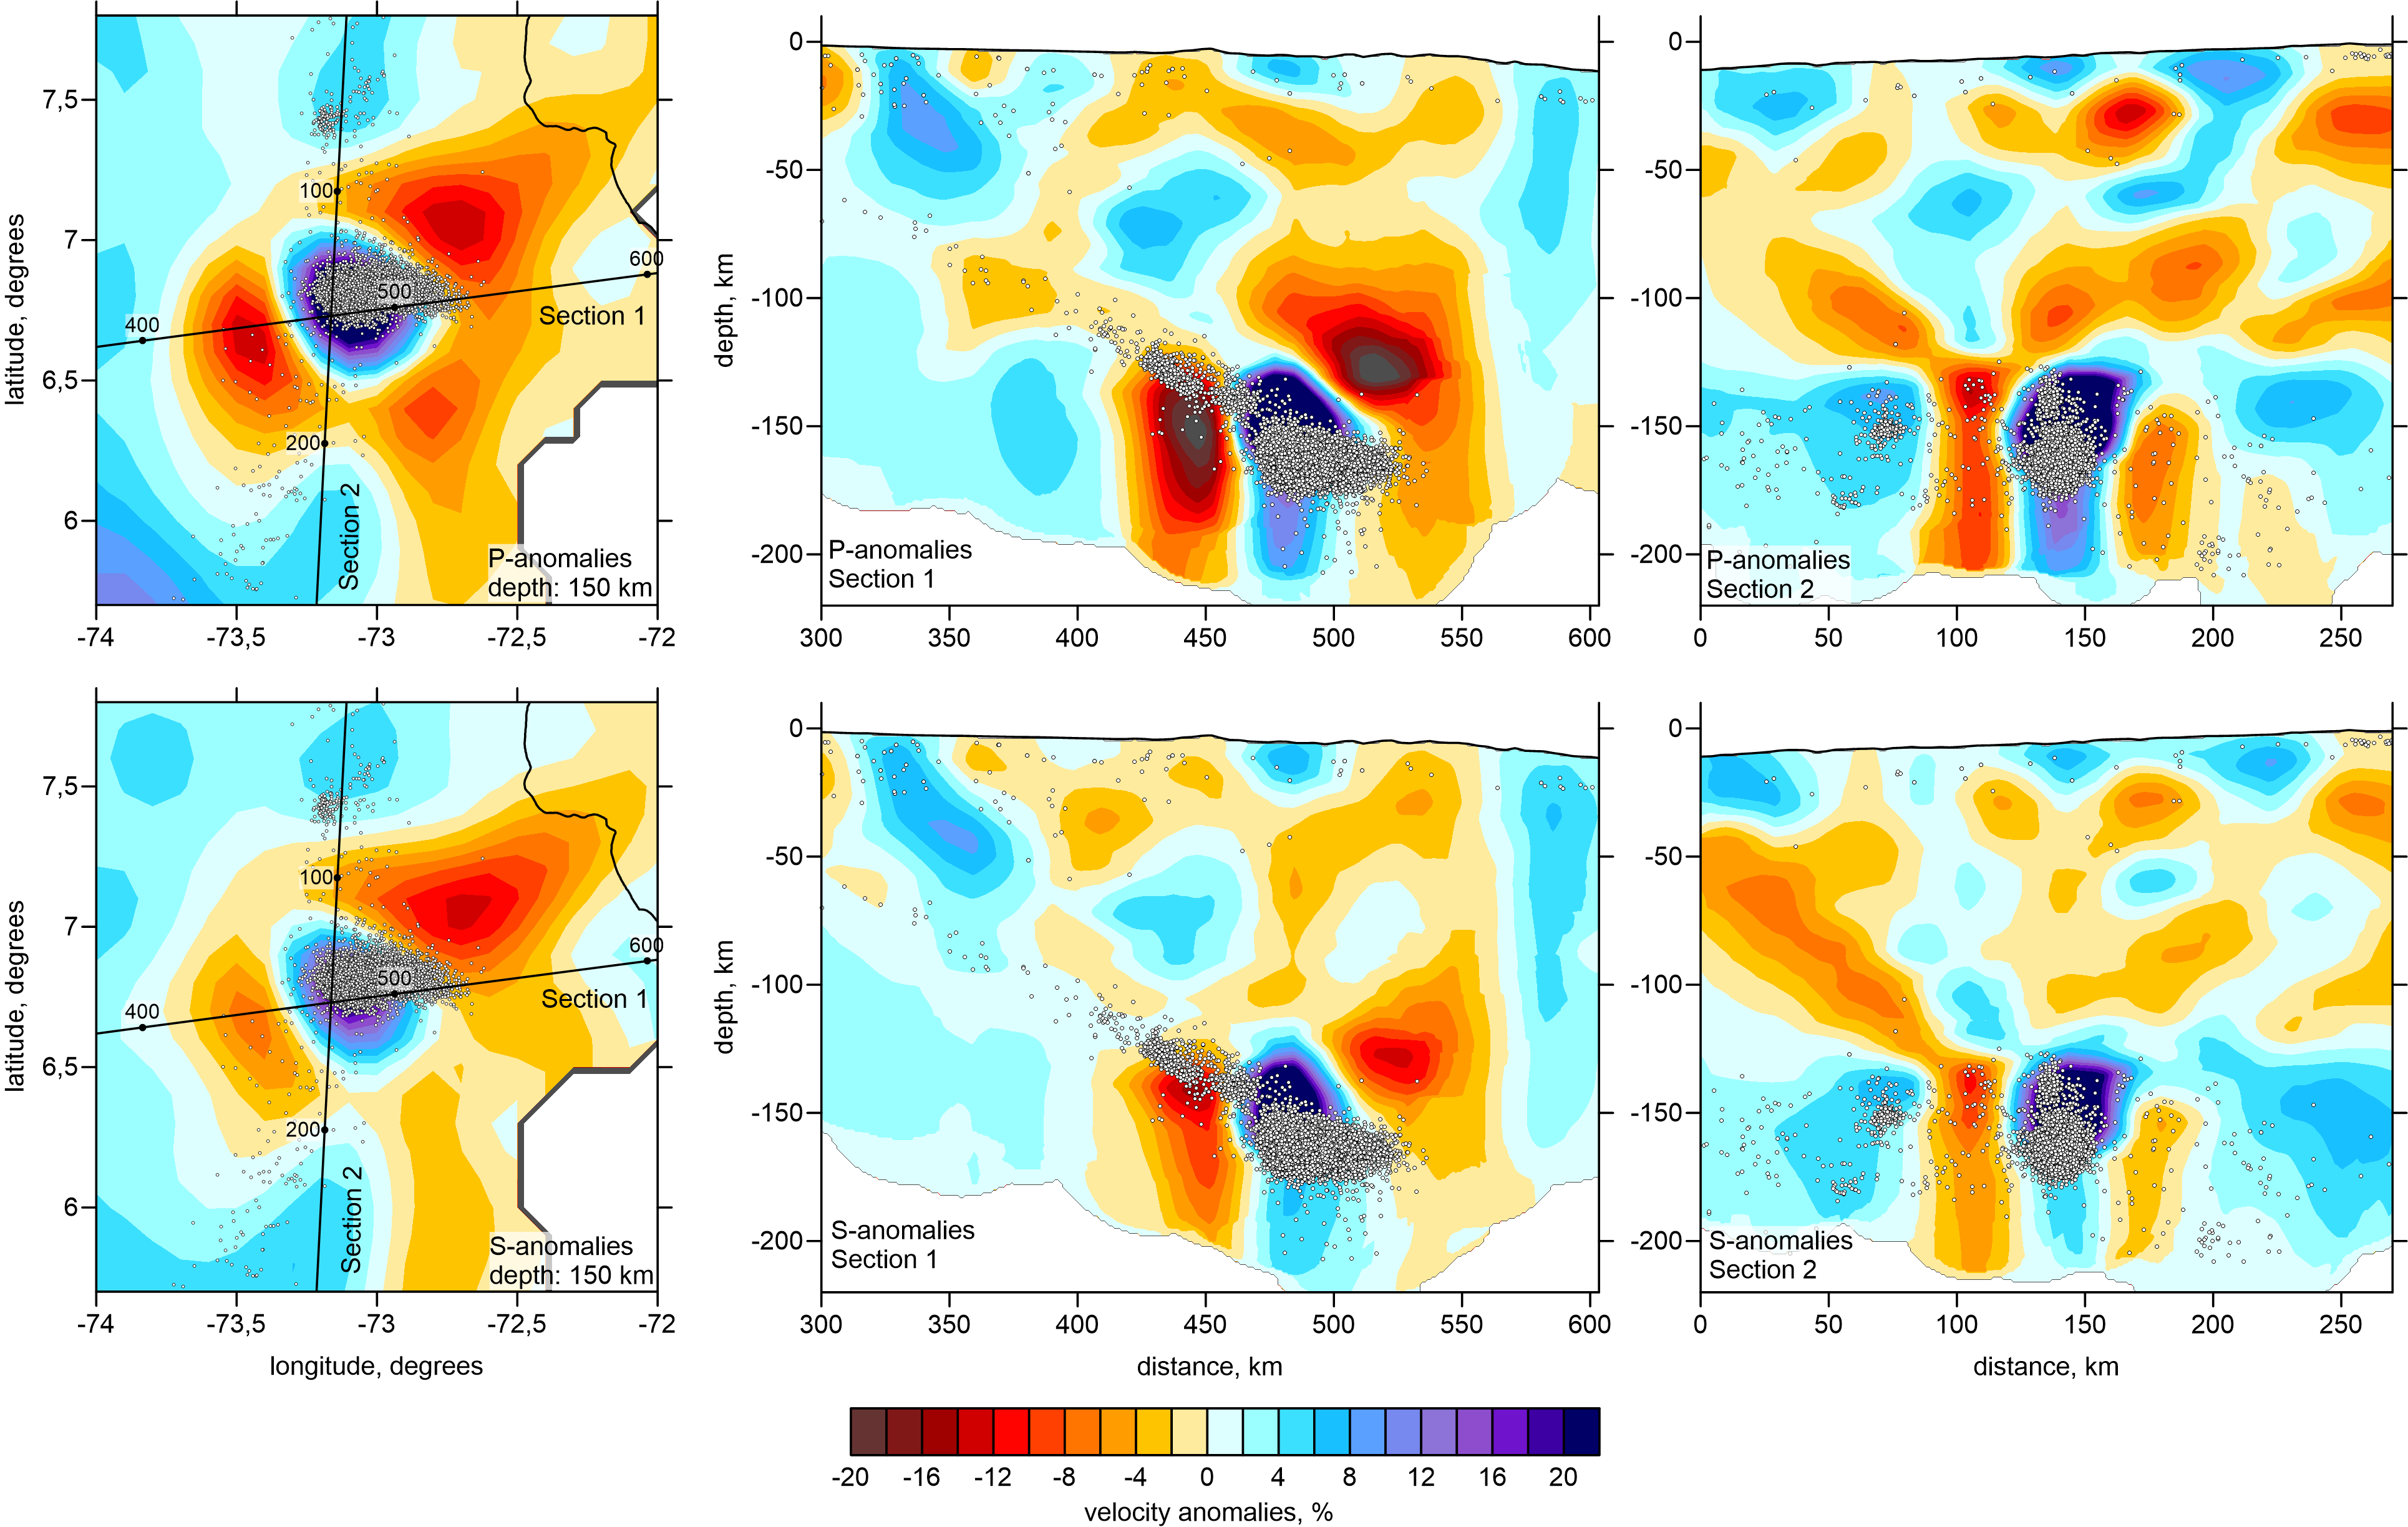
\includegraphics[scale=0.45]{deep_anomaly_hor_ver.png}
\label{fig:seism_data}
\end{figure}

\section{Geophysical Model}

The skill how to correctly model geophysics for a numerical simulation is to vast that it could fit into a single book much less into a simple report. A good starting point which is essential to understand this project is the book "Introduction to Numerical Geodynamic Modelling" \cite{gerya2009introduction} written by Taras Gerya. This project can also be seen as an additional example in application of geophysical numerical modeling.

\subsection{Physical Equations}
For completeness all equations used in the simulation are listed below. Most equations originate from the fact that the material is seen as a continuum. Therefore one can intuitively guess that the three conservation laws are used for describing its behavior. Namely the conservation of mass, momenta and energy or in this case heat. First the conservation of mass is described by the continuity equation written as:
\begin{align}
\frac{d \rho}{d t} + \nabla \cdot (\rho \mathbf{v})&=0\\
\frac{D \rho}{D t} + \rho \nabla \cdot \mathbf{v}&=0
\end{align}
in Eulerian and Lagrangian form where $\rho$ is the local density of the material and $\mathbf{v}=\begin{pmatrix}v_x\\v_y \end{pmatrix}$ the local velocity.

The second law, conservation of momenta, is described by the Navier-Stokes equations. Since this project is a model in two dimensions the reduced Naver-Stokes equation in Eulerian form is written as:
\begin{align}
\frac{\partial \sigma_{xx}'}{\partial x}+\frac{\partial \sigma_{xy}}{\partial y}-\frac{\partial P}{\partial x}+\rho g_x&=\rho \left( \frac{\partial v_x}{\partial t}+v_x\frac{\partial v_x}{\partial x}+v_y\frac{\partial v_x}{\partial y} \right)\\
\frac{\partial \sigma_{yy}'}{\partial x}+\frac{\partial \sigma_{yx}}{\partial y}-\frac{\partial P}{\partial y}+\rho g_y&=\rho \left( \frac{\partial v_y}{\partial t}+v_x\frac{\partial v_y}{\partial x}+v_y\frac{\partial v_y}{\partial y} \right)\\
\intertext{and in Lagrangian form as:}
\frac{\partial \sigma_{xx}'}{\partial x}+\frac{\partial \sigma_{xy}}{\partial y}-\frac{\partial P}{\partial x}+\rho g_x&=\rho \frac{D v_x}{D t}\\
\frac{\partial \sigma_{yy}'}{\partial x}+\frac{\partial \sigma_{yx}}{\partial y}-\frac{\partial P}{\partial y}+\rho g_y&=\rho \frac{D v_y}{D t}\\
\end{align}
Last but not least the third conservation law, conservation of heat, also known as temperature equation, can be derived from Fourier's law of heat conduction and has the following Lagrangian form, assuming $k$ is constant:
\begin{align}
\rho C_p \frac{D T}{D t} &= k (\frac{\partial^2 T}{\partial x^2}+\frac{\partial^2 T}{\partial y^2})+H_r+H_s+H_a+H_L\\
\intertext{or in Eulerian form:}
\rho C_p (\frac{\partial T}{\partial t}+v_x \frac{\partial T}{\partial x} + v_y \frac{\partial T}{\partial y})&= k (\frac{\partial^2 T}{\partial x^2}+\frac{\partial^2 T}{\partial y^2})+H_r+H_s+H_a+H_L
\intertext{In this project only two heating terms are considered relevant namely the adiabatic heating $H_a$ and the shear heating $H_s$. These two are approximated with the following relations:}
H_a &\approx \alpha\cdot T \cdot v_y \cdot \rho \cdot g_y\label{eq:ha}\\
H_s &\approx \sigma_{xx}\cdot \dot{\epsilon}_{xx} + \sigma_{xy}\cdot \dot{\epsilon}_{xy}\label{eq:hs}
\end{align}
All these equations have in common namely that they are all partial differential equations in space and time where mostly an analytical solution cannot be found. Furthermore to find a solution on a domain one requires additional information such as the initial state and boundary conditions.

With these tree equation one can depict how the continuum moves and how the temperature develops but what is still missing is the behavior of the material under these changes. This is defined in the rheology of rocks. There are a lot of possible choices for the behavior like visco-elastic, visco-plastic etc. to name just a few. In this project for simplicity the well-known empirical rheological relationship was used \ref{eq:emprheolrel} between strain-rate and differential stress which is of the following form:
\begin{equation}
\dot{\gamma}=A_D h^m (\sigma_d)^n\exp\left( -\frac{E_a+V_a P}{RT} \right)
\label{eq:emprheolrel}
\end{equation}
Note however that $A_D,h,E_a$ and $V_a$ are still parameters which have to be defined. A sensible choice will be shown in section \ref{seq:modelsetup} about the model setup. As already shown in equation \ref{eq:ha} and \ref{eq:hs} the standard definition of stress, strain and strain-rate are mandatory for the description which is listed next in addition with the property for isotropic, incompressible materials \ref{eq:iim}.
\begin{align}
\sigma_{ij}'&=\sigma_{ij}+P\delta_{ij}\\
\sigma_{\RN{2}}&=\sqrt{\frac{1}{2}(\sigma_{ij}')^2}\\
\epsilon_{ij}&=\frac{1}{2}\left( \frac{\partial u_i}{\partial x_j}+\frac{\partial u_j}{\partial x_i}\right)\\
v_i&=\frac{D u_i}{D t}\\
\dot{\epsilon_{ij}}&=\frac{1}{2}\left( \frac{\partial v_i}{\partial x_j}+\frac{\partial v_j}{\partial x_i}\right)\\
\dot{\epsilon}_{ij}'&=\dot{\epsilon}_{ij}-\delta_{ij}\frac{1}{3}\dot{\epsilon}_{kk}\\
\dot{\epsilon}_{kk}&=\nabla \cdot \mathbf{v}\\
\dot{\epsilon}_{\RN{2}}&=\sqrt{\frac{1}{2}(\dot{\epsilon}_{ij}')^2}\\
\sigma_{\RN{2}} &= 2 \eta_{eff}\dot{\epsilon}_{\RN{2}}\label{eq:iim}
\end{align}
%Also the property for isotropic, incompressible materials \ref{eq:iim} will be utilized.
%\begin{equation}
%\label{eq:iim}
%\end{equation}

\section{Model setup}
\label{seq:modelsetup}
First of all the model setup for a subduction zone will be shown as a basis. This model is utilized for simulating the subduction of a slab from the lithosphere into the asthenosphere. Depending on the properties of the necking area different scenarios occur. The actual model of this project takes a segment of this model and places a "cold plume" above the slab. In this model the interest lies not in the process of breaking of the slab but in the interaction between the slab and the plume where different tendencies develop.
\subsection{Model of a subduction zone}
The model of a subduction zone consists of three layers. Namely the water layer, the lithosphere and the asthenosphere. These layers are shown in figure \ref{fig:modelsubductionzone}. The green section describes the necking are which determines the development of the simulation. To get a complete problem the parameters and rheology has to be characterized for all layers in addition also the initial state and boundary conditions have to be chosen. A standard model is described as follows:

\begin{tabular}{lll}
layer&property&value\\
water&&\\
&density $\rho$&$1000 [\frac{kg}{m^3}]$\\
&temperature $T$&$273[K]$\\
&viscosity $\eta$&$10^{18} [Pa\cdot s]$\\
&thermal conductivity $k$&$300 [\frac{W}{m\cdot K}]$\\
&heat capacity $C_p$&$3000 [\frac{J}{kg\cdot K}]$\\
&thermal expansion $\alpha$&not needed$[\frac{1}{K}]$\\
&compressibility $\beta$&not needed$[\frac{1}{Pa}]$\\
&stress strength $\sigma_{yield}$&not needed$[\frac{J}{m^3}]$ \\
lithosphere&&\\
&density $\rho$&$3300 [\frac{kg}{m^3}]$\\
&temperature $T$&$T(y) [K]$\\
&viscosity $\eta$&$10^{23} [Pa\cdot s]$\\
&thermal conductivity $k$&$k(T) [\frac{W}{m\cdot K}]$\\
&heat capacity $C_p$&$1000 [\frac{J}{kg\cdot K}]$\\
&thermal expansion $\alpha$&$3\cdot10^{-5}[\frac{1}{K}]$\\
&compressibility $\beta$&$10^{-11}[\frac{1}{Pa}]$\\
&stress strength $\sigma_{yield}$&$5\cdot 10^7[\frac{J}{m^3}]$ \\
asthenosphere&&\\
&density $\rho$&$3250 [\frac{kg}{m^3}]$\\
&temperature $T$&$1500 [K]$\\
&viscosity $\eta$&$10^{19} [Pa\cdot s]$\\
&thermal conductivity $k$&$k(T) [\frac{W}{m\cdot K}]$\\
&heat capacity $C_p$&$1000 [\frac{J}{kg\cdot K}]$\\
&thermal expansion $\alpha$&$3\cdot10^{-5}[\frac{1}{K}]$\\
&compressibility $\beta$&$10^{-11}[\frac{1}{Pa}]$\\
&stress strength $\sigma_{yield}$&$5\cdot 10^7[\frac{J}{m^3}]$ \\
\end{tabular}

\begin{align}
T(y) &= \frac{(1500 - 273)}{50} \cdot (y - 50) + 273\\
k(T) &= 0.73 + \frac{1293}{T+77}\\
\rho(\beta,\alpha,P,T)&=3300\cdot \frac{1+\beta \cdot (P-P_0)}{1+\alpha \cdot (T-T_0)}\\
\epsilon_{\RN{2}}&=\sqrt{0.5\cdot(\dot{\epsilon}_{xx}^2+\dot{\epsilon}_{yy}^2)+\dot{\epsilon}_{xy}^2 }\\
\eta(A_D,n,V_a,E_a,T,P,\epsilon_{\RN{2}})&=\frac{0.5}{A_D^{\frac{1}{n}}}\cdot \epsilon_{\RN{2}}^{\frac{1}{n}-1}\cdot \exp{\frac{(E_a+P\cdot V_a)}{R\cdot T \cdot n}}
\end{align}

\begin{tabular}{llll}
rock type&parameter&value&zone\\
dry olivin&&&lithosphere and slab\\
&$A_D$&$2.5\cdot 10^{-17}$&\\
&$n$&$3.5$&\\
&$V_a$&$8\cdot 10^{-6}$&\\
&$E_a$&$532000$&\\
wet olivin&&&asthenosphere\\
&$A_D$&$2\cdot 10^{-21}$&\\
&$n$&$4$&\\
&$V_a$&$4\cdot 10^{-6}$&\\
&$E_a$&$471000$&\\
\end{tabular}

\begin{figure}
\includegraphics[scale=0.8]{model1.pdf}
\caption{model structure of subduction zone}
\label{fig:modelsubductionzone}
\end{figure}

\begin{tabular}{ll}
constant&value\\
universal gas constant $R$&$8.314$\\
viscosity cutoff $\eta_{min}$&$10^{16}$\\
viscosity cutoff $\eta_{max}$&$10^{24}$\\
standard temperature $T_0$&$273[K]$\\
standard pressure $P_0$&$10^5 [Pa]$\\
\end{tabular}

At this step the model description for the initial state, the rheology and the constants are all defined. What is missing is the boundary condition used for solving the temperature and Navier-Stokes equations. For the Navier-Stokes solver there many possible choices but only two are presented here. These are the no slip and free slip boundary conditions.

\begin{tabular}{ll}
boundary condition&property\\
no slip&$v_x=0$ and $v_y=0$ everywhere on the boundary\\
free slip&\makecell[l]{ $\frac{\partial v_y}{\partial x}=0$ and $v_x=0$ on boundaries parallel to y-axis\\$\frac{\partial v_x}{\partial y}=0$ and $v_y=0$ on boundaries parallel to x-axis }
\end{tabular}\\
%$\frac{\partial v_y}{\partial x}=0$ and $v_x=0$ on boundaries parallel to y-axis\newline$\frac{\partial v_x}{\partial y}=0$ and $v_y=0$ on boundaries parallel to x-axis\\
For the temperature equation first of all a linear gradient in the lithosphere was chosen from $273K$ to $1500K$ which is also present in the slab. For the top and bottom boundary which are parallel to the x-axis a constant heating boundary condition was selected with $273K$ and $1500K$ respectively. For the left and right boundary parallel to the y axis thermal insulation was the most sensible choice, meaning the temperature is set equal to the temperature from the neighboring grid point on the right/left.

Since the solvers for the Navier-Stokes and temperature equations work only on discrete grids the model is also solved only on the grid points. Therefore the choice of how the grid is defined influences the whole simulation process. In this project the same staggered grid as explained in \cite{gerya2009introduction} was used. Thus the properties are fixed on material points like in the Lagrangian view which will be interpolated on to the fixed grid which will be shortly explained in the implementation section \ref{seq:impl}.

\subsection{Model of this project}
Now the actual domain of this project refines the above model on to a smaller domain with an additional "cold plume" as roughly indicated with the white borders in figure \ref{fig:modelsubductionzone}. The new model is shown in figure \ref{fig:tm}. Therefore all previously mentioned properties, constants and equations can be transfered on to the new model but note that some are slightly modified which will be listed next. Since there is no longer a water layer these properties can be ignored in this model and the properties of the "cold plume" has to be added which are the following:

\begin{tabular}{lll}
plume&&\\
&density $\rho$&$3500 [\frac{kg}{m^3}]$\\
&temperature $T$&$700 [K]$\\
&viscosity $\eta$&$10^{23} [Pa\cdot s]$\\
&thermal conductivity $k$&$k(T) [\frac{W}{m\cdot K}]$\\
&heat capacity $C_p$&$1000 [\frac{J}{kg\cdot K}]$\\
&thermal expansion $\alpha$&$3\cdot10^{-5}[\frac{1}{K}]$\\
&compressibility $\beta$&$10^{-11}[\frac{1}{Pa}]$\\
&stress strength $\sigma_{yield}$&$p_3 [\frac{J}{m^3}]$ \\
\end{tabular}

Since the goal of this project is to see the different tendencies of this setup $\sigma_{yield}$ is varied as a parameter $p_3$. $p_3$ is assigned to take on $10^7$, $2\cdot 10^7$, $5\cdot 10^7$, or $10^8$. The first parameter $p_1$ is the actual starting position of the plume $(x_p,y_p)$ marked as yellow in figure \ref{fig:tm}. This position was varied across three types. First where the plume has not much space on the left side and is near the contact point with the slab. Second in the middle of the slab where enough space is on both sides and the contact point is near or far away. And lastly the third position is near the edge of the slab and has the most distance to the contact point.
The second parameter $p_2$ is the angle $\gamma$ of the slab shown in green. The angle was chosen to be $20$, $30$, $45$ or $60$ degree. The forth parameter $p_4$ is $\sigma_{yield}$ of the buffer zone marked as bright blue in figure \ref{fig:tm}. This can take on the same values as $p_3$. The last and fifth parameter $p_5$ of the model is the radius of the plume indicated as white in figure \ref{fig:tm}. The radius is assigned to be $10$, $15$, $20$, $25$ or $30$ kilometers. A vigilant reader can guess that the number of simulations can exceed $1000$ possibilities. Therefore only different tendencies are reported in the results section. The code of this project will be online obtainable for the interested reader to try different simulations himself. A warning is here issued since one simulation can take up to $30$ minutes and it is not guaranteed that all quantities remain physically meaningful since numerical errors amplify with time.

\begin{figure}[!ht]
\includegraphics[scale=1.2]{model2.pdf}
\label{fig:tm}
\caption{model of this project}
\end{figure}

A significant difference to the previous model is that in the rest of the domain where $p_3$ or $p_4$ is not used the $\sigma_{yield}$ strength is made pressure dependent. The function has the following form:
\begin{equation}
\sigma_{yield}(P) = 3\cdot 10^6+0.6 \cdot P
\end{equation}
This corresponds better to our intuition since rock under high pressure in equilibrium is sturdy until it is broken when the pressure exceeds the material threshold. For this model only the free slip boundary condition was considered in the Navier-Stokes solver since it is a refinement of the model before. Whereas for the temperature equation thermal insulation was used on all borders. This implies that the energy of the system will fall slowly since numerical diffusion is present in such simulations with finite difference schemes. Now is everything defined to start a simulation. How the simulation is structured is explained in implementation section \ref{seq:impl}.  


\section{Implementation}
\label{seq:impl}
The actual implementation in matlab is to long to show the complete code. Therefore the functionality will be explained with the following flow diagram figure \ref{fig:flow}. The black boxes signifies the stages in the algorithm and the blue text the effect respectively which variable is now available for use.

\begin{figure}[!ht]
\includegraphics[scale=1.0]{tikz.pdf}
\caption{flow diagram of the algorithm}
\label{fig:flow}
\end{figure}

Noteworthy in this framework is that two whole solvers for partial differential equations are used. To briefly mention the functionality they are based on solving the system of equations composed out of finite difference schemes and boundary conditions with the matlab internal backslash operator. In the first solver the velocity fields $v_x$ and $v_y$ are unknown together with the pressure $P$. In the second only the temperature $T$ is unknown and therefore the number of equations is three times smaller than in the Navier-Stokes solver. For a more detailed explanation on the functionality the same book \cite{gerya2009introduction} is recommended.

\section{Results}
The whole simulation time depending on the stability is approximately around 100-200 million years. In this context only the first two million years are considered relevant for matching the profile of the data. The rest of the data is a lookout for the longterm tendency. Of interest here are three things. First is the velocity profile of the plume dependent on the parameters. Second is the rotation of the plume dependent on the parameters. The third and last is the effect of pushing material in front of the plume like a bulldozer which can correspond to the data.
\subsection{Initial State}
Shown in figure \ref{fig:initial} are the initial states of the simulations for the reference position. In each of the figures six properties are presented. The top leftmost picture represent different types of materials. The light and dark blue represent the same type but is used to demonstrate rotation. Therefore one can see four different kinds of materials. The top middle figure is the temperature and top right is the viscosity. At the bottom there is on the left the shear heating, in the middle the second strain invariant, and on the right the $v_y$ velocity including arrows for both $v_x$ and $v_y$ velocities. At the bottom annotated is the next time step $\Delta t$ and the current absolute time.

\begin{figure}[!ht]
	\begin{minipage}[t]{1.0\textwidth}
		\begin{minipage}[t]{0.5\textwidth}
			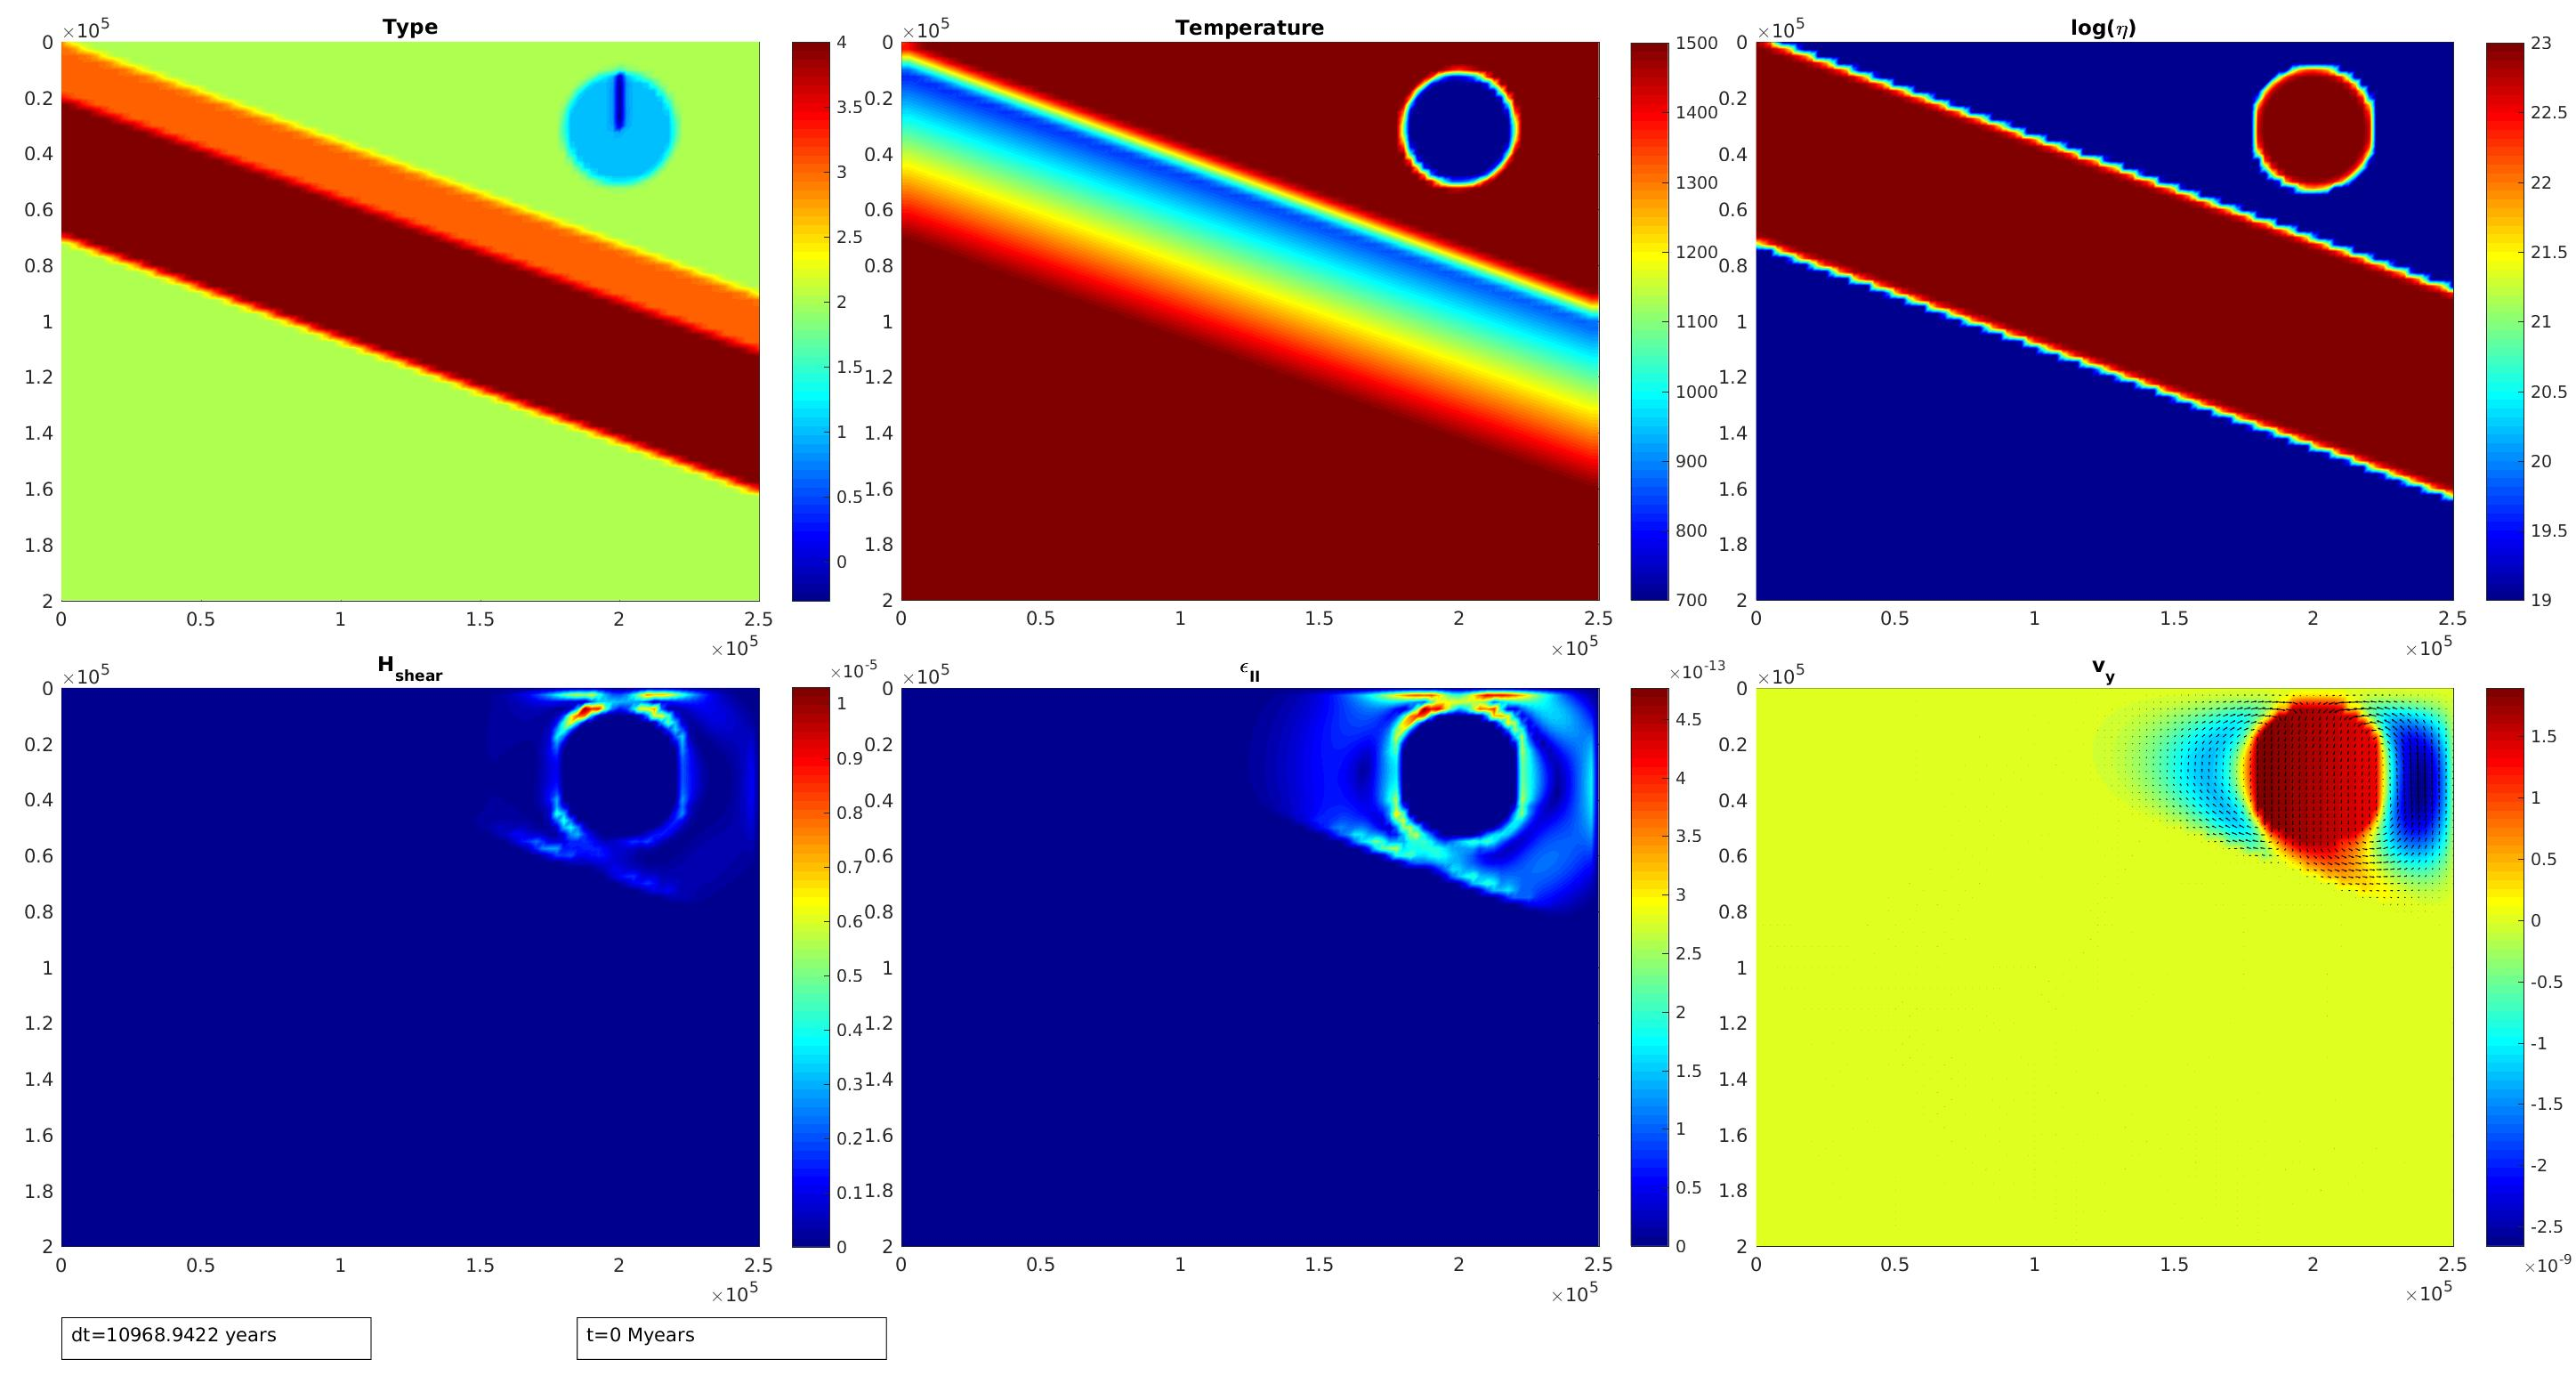
\includegraphics[width=1.0\textwidth]{./Snapshots/ref/Subductionzonewithblob1posrefslab20s2e7s2e7r20.jpg}
		\end{minipage}
		\begin{minipage}[t]{0.5\textwidth}
			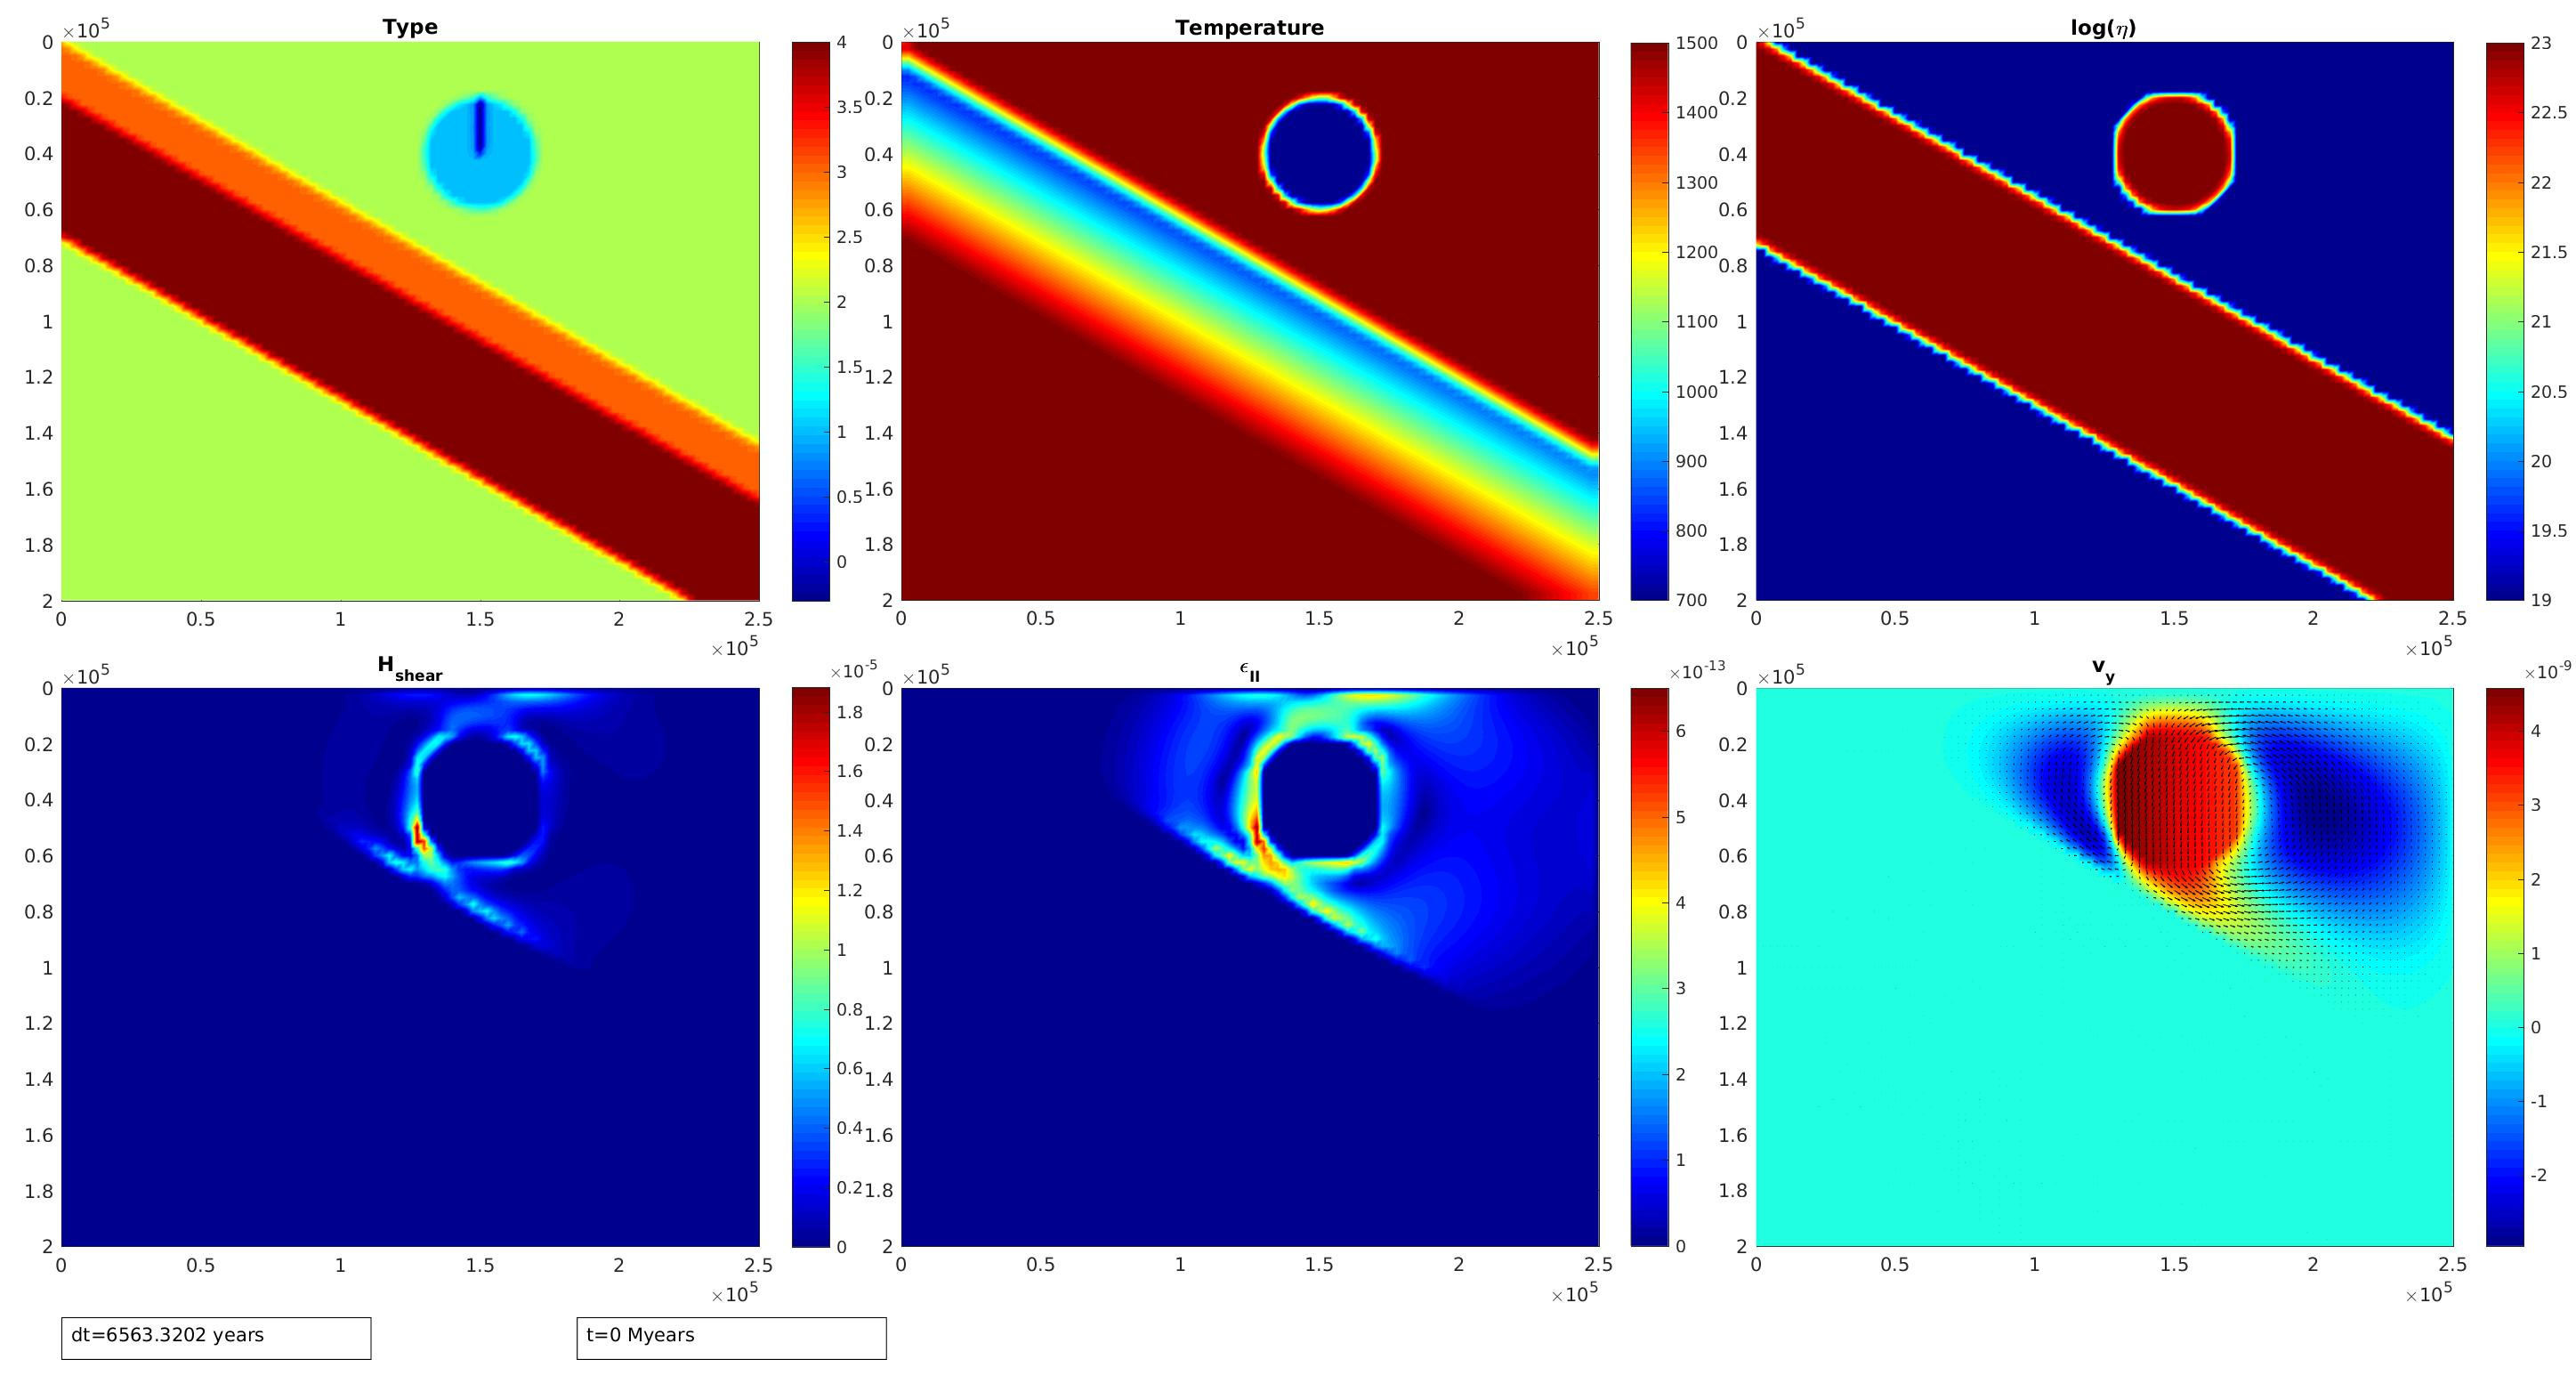
\includegraphics[width=1.0\textwidth]{./Snapshots/ref/Subductionzonewithblob1posrefslab30s2e7s2e7r20.jpg}
		\end{minipage}
	\end{minipage}
	\begin{minipage}[c]{1.0\textwidth}
		\begin{minipage}[t]{0.5\textwidth}
			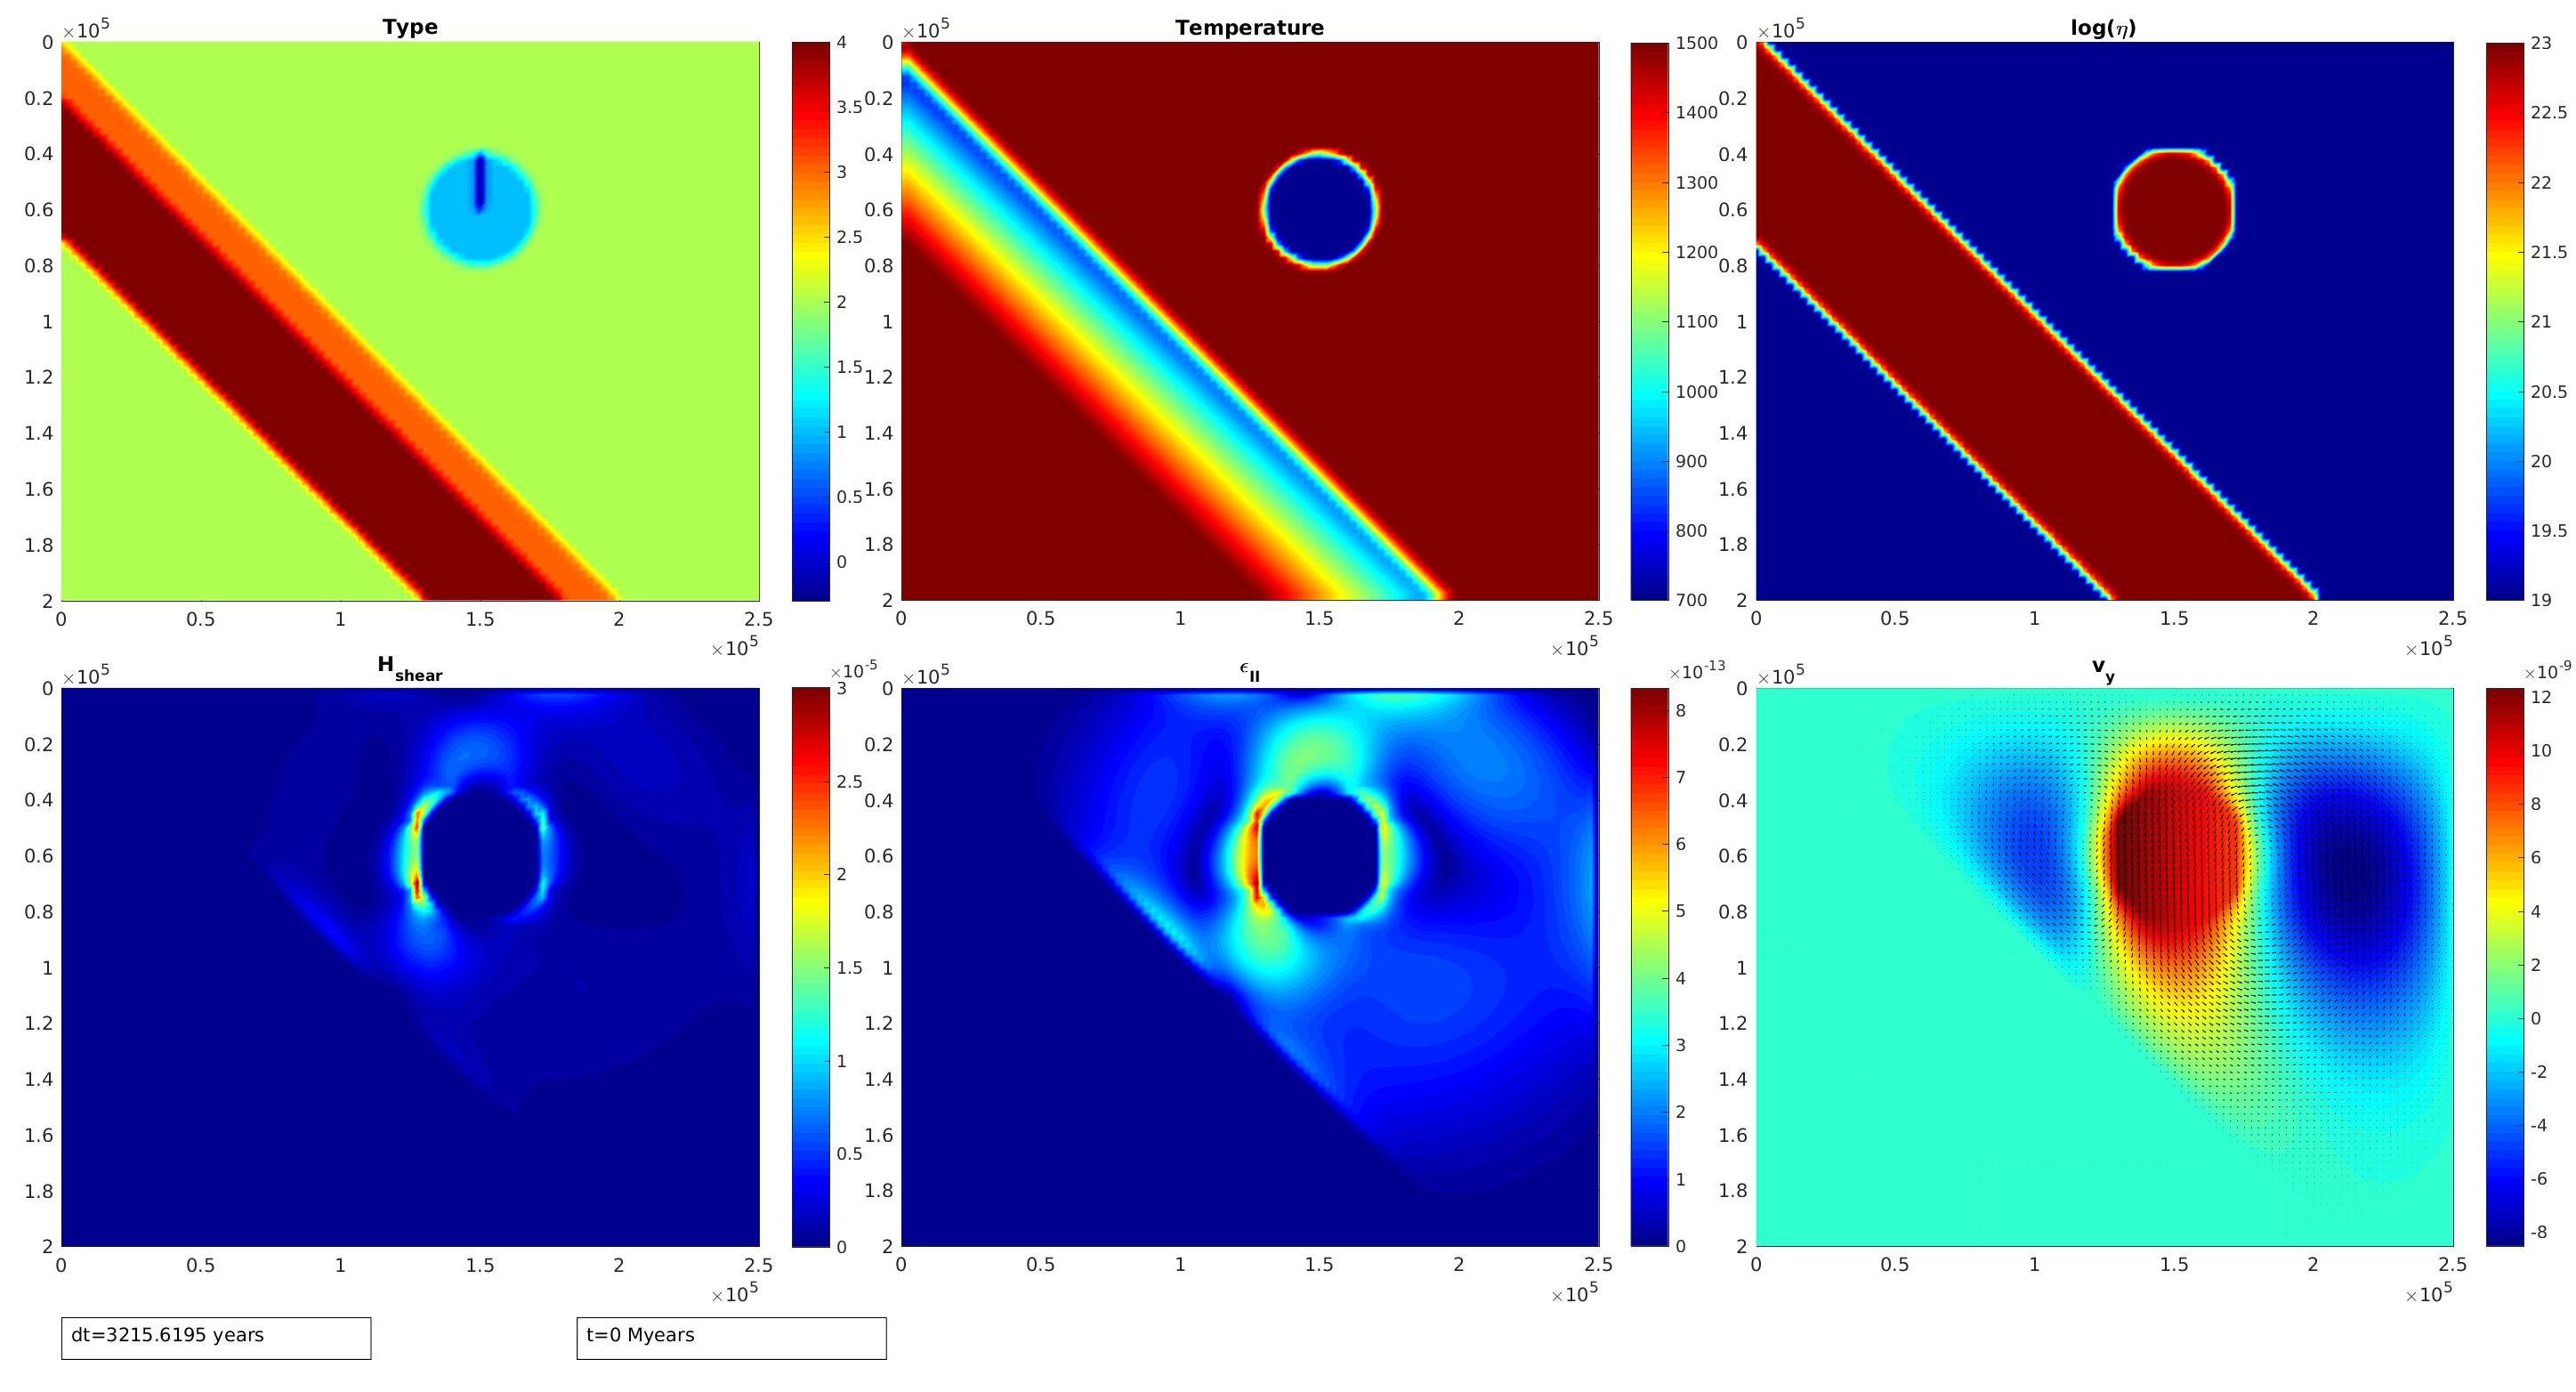
\includegraphics[width=1.0\textwidth]{./Snapshots/ref/Subductionzonewithblob1posrefslab45s2e7s2e7r20.jpg}
		\end{minipage}
		\begin{minipage}[t]{0.5\textwidth}
			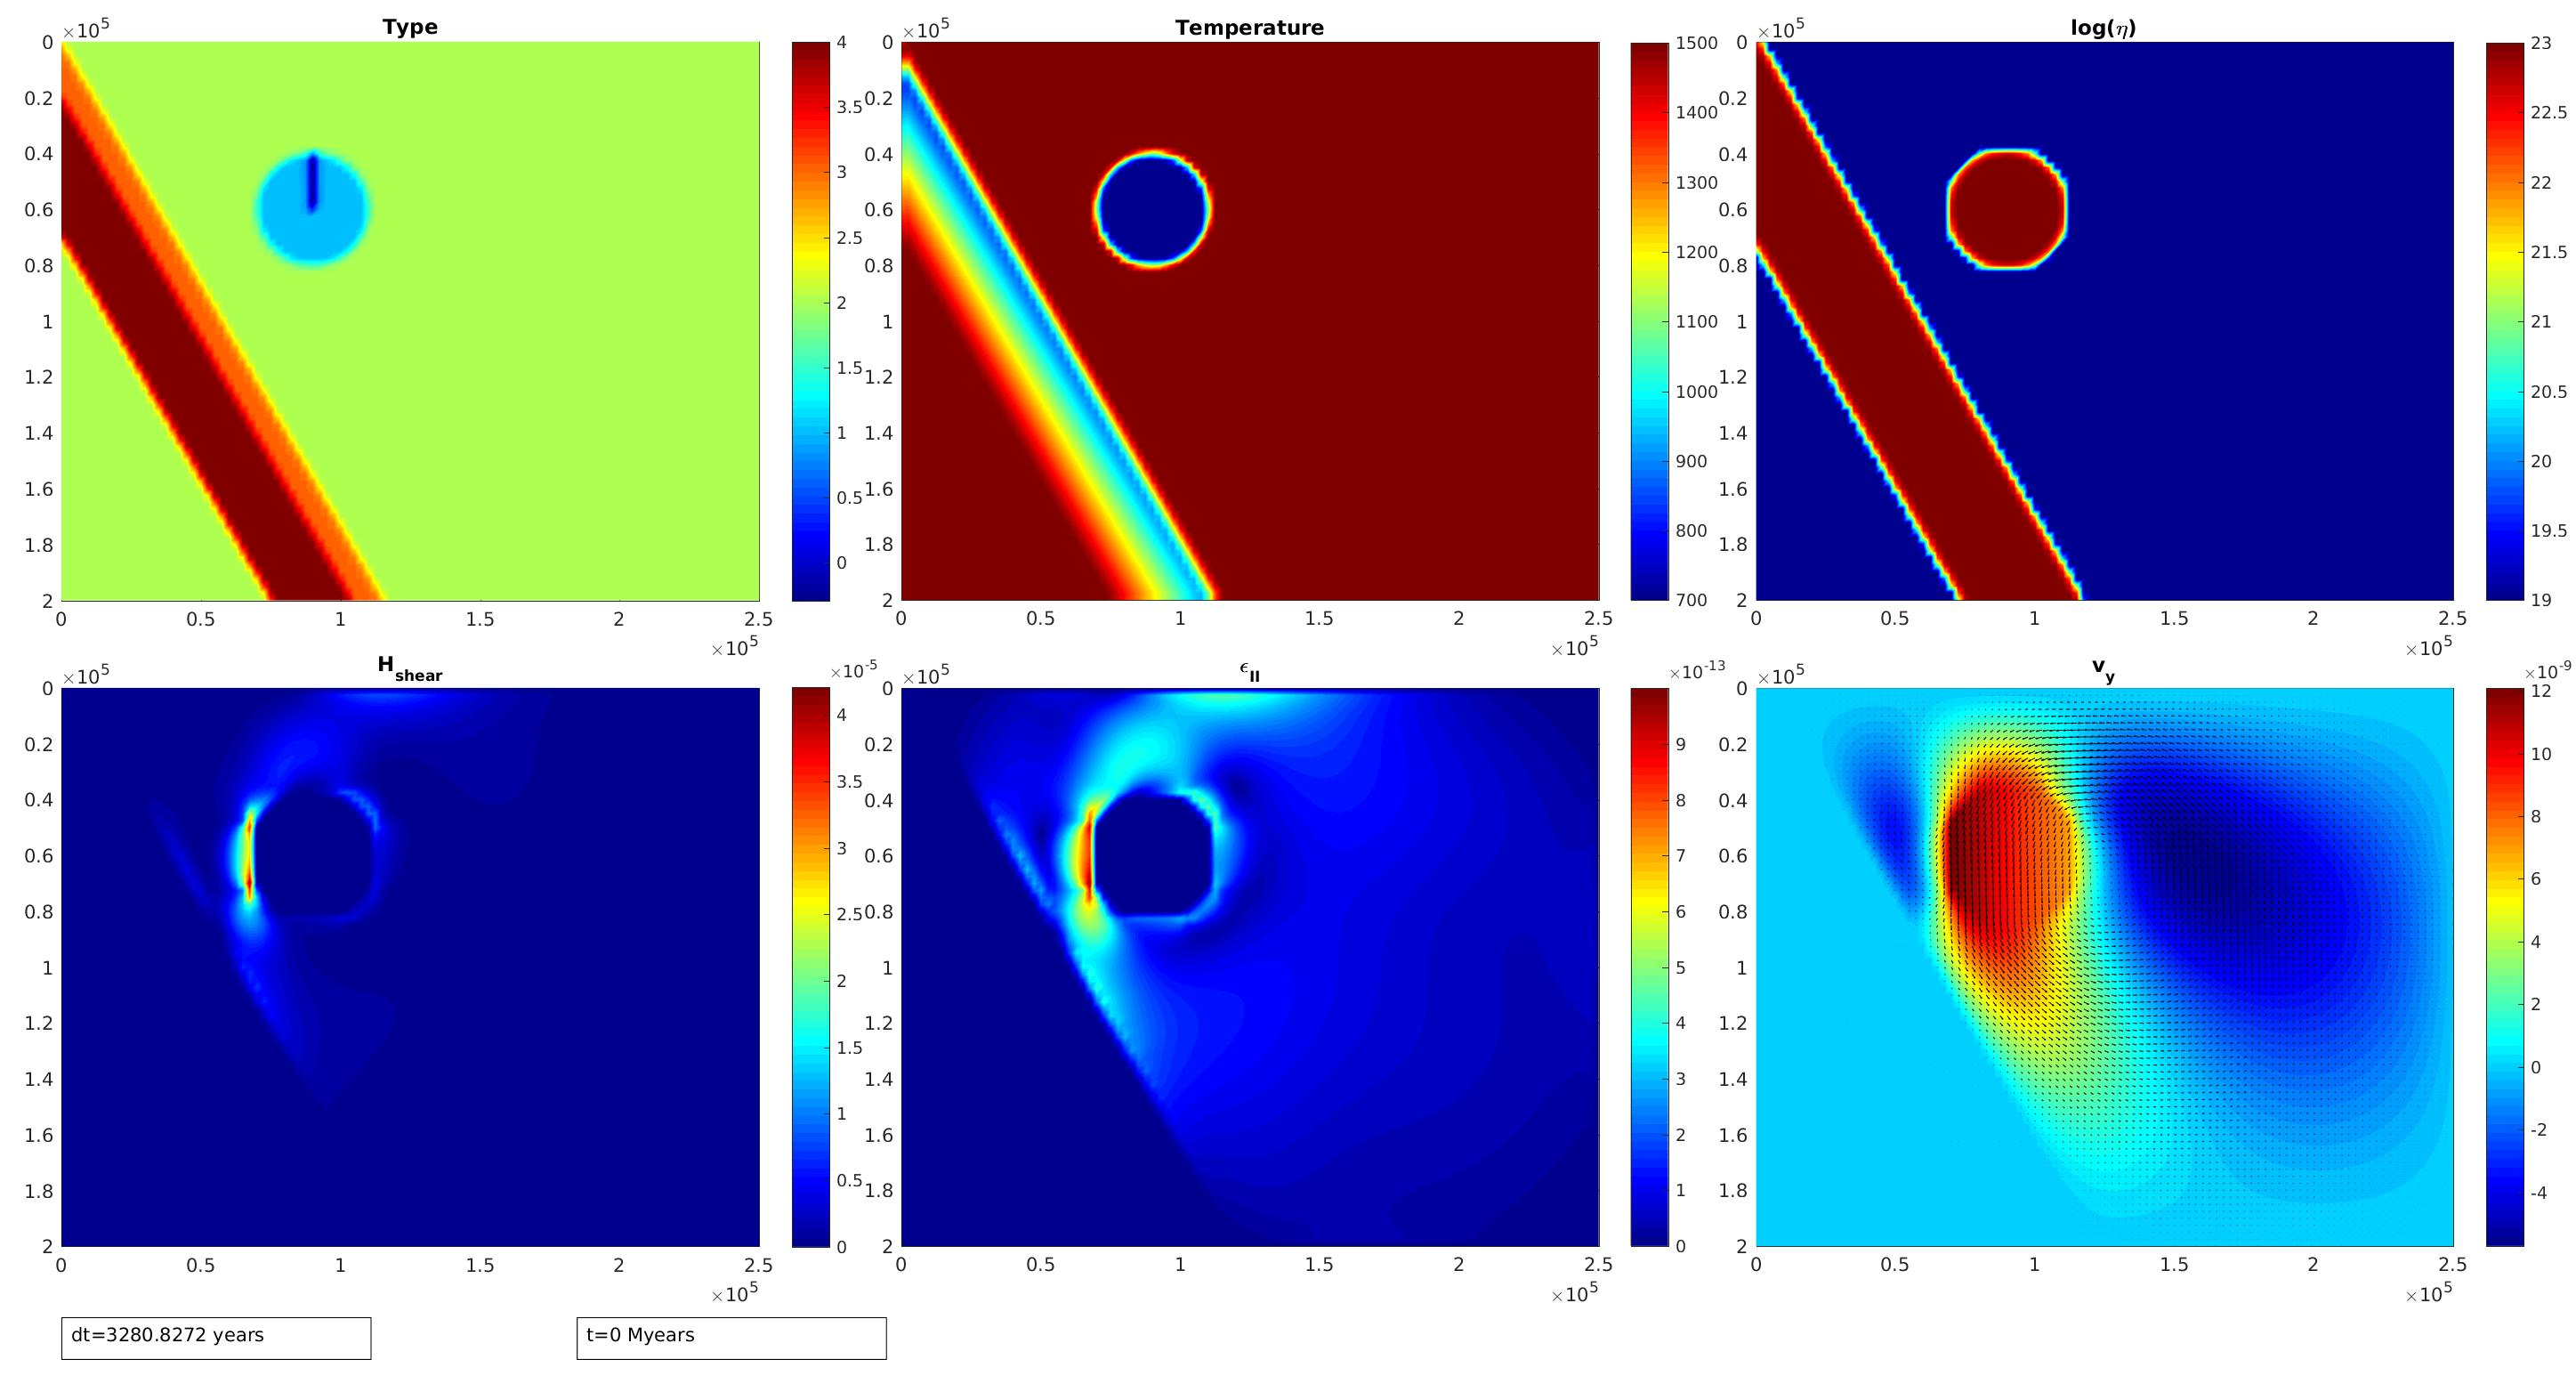
\includegraphics[width=1.0\textwidth]{./Snapshots/ref/Subductionzonewithblob1posrefslab60s2e7s2e7r20.jpg}
		\end{minipage}
	\end{minipage}
	\caption{Initial reference state for 20, 30, 45 and 60 degree slope}
	\label{fig:initial}
\end{figure}

Please note that in the case of 20 degree slope not much space is left to play with the position. Additionally in case of 60 degree slope there is enough space but would not collide with the plate. Therefore such scenarios also will not be considered. In figure \ref{fig:initial} only the reference radius of 20 kilometers is depicted and variation in the strength properties will not change these plots only their behavior. 

\subsection{Equal strength of plate and plume}
The first scenario to look at is when the strength of the plate and the plume is equal. Intuitively what is expected to happen is that the plume will be deflected and will glide over plate with some small deformations. And indeed this was the case as shown in figure \ref{fig:2m20}, \ref{fig:2m30}, \ref{fig:2m45} and \ref{fig:2m60}. The longterm results are shown afterwards in the figures \ref{fig:100t20}, \ref{fig:100t30}, \ref{fig:100t45} and \ref{fig:150t60}. Here one can see problems in the 20deg and 30deg case since the plate was deformed like a snake which is not physical real behavior and therefore such scenarios are considered impossibilities since they occur because of the limited model space. The reason of deformation is that there is not enough space where material can escape to and therefore when the plume moves pressure is build up on the plate until it deforms. Interestingly there is also a special case when the plate and plume have not an reference strength of $2\cdot 10^7$ but only $1\cdot 10^7$ and the plume has a radius of $10$ kilometers then the plume can dig through the plate shown in figure \ref{fig:150t2010km}. Another effect what could happen is that the plume is to close to the top boundary and therefore sticks to long to that position what is illustrated in figure \ref{fig:3m3025km}. Also the desired bulldozer effect is possible to realize in this setting although both plate and plume have the same strength shown in figure \ref{fig:55m3015km}. The only problem here is that the effect occurs only after 55 million years has passed in comparison to the timeframe of 2 million years which is considered relevant. Therefore later on a section for only mixed strength is used for this endeavor to search for the bulldozer effect. The next two sections is devoted to examine the rotation and velocity profile of the plume for the in figure \ref{fig:initial} shown reference plots.

\begin{figure}
\begin{minipage}[t]{1.0\textwidth}
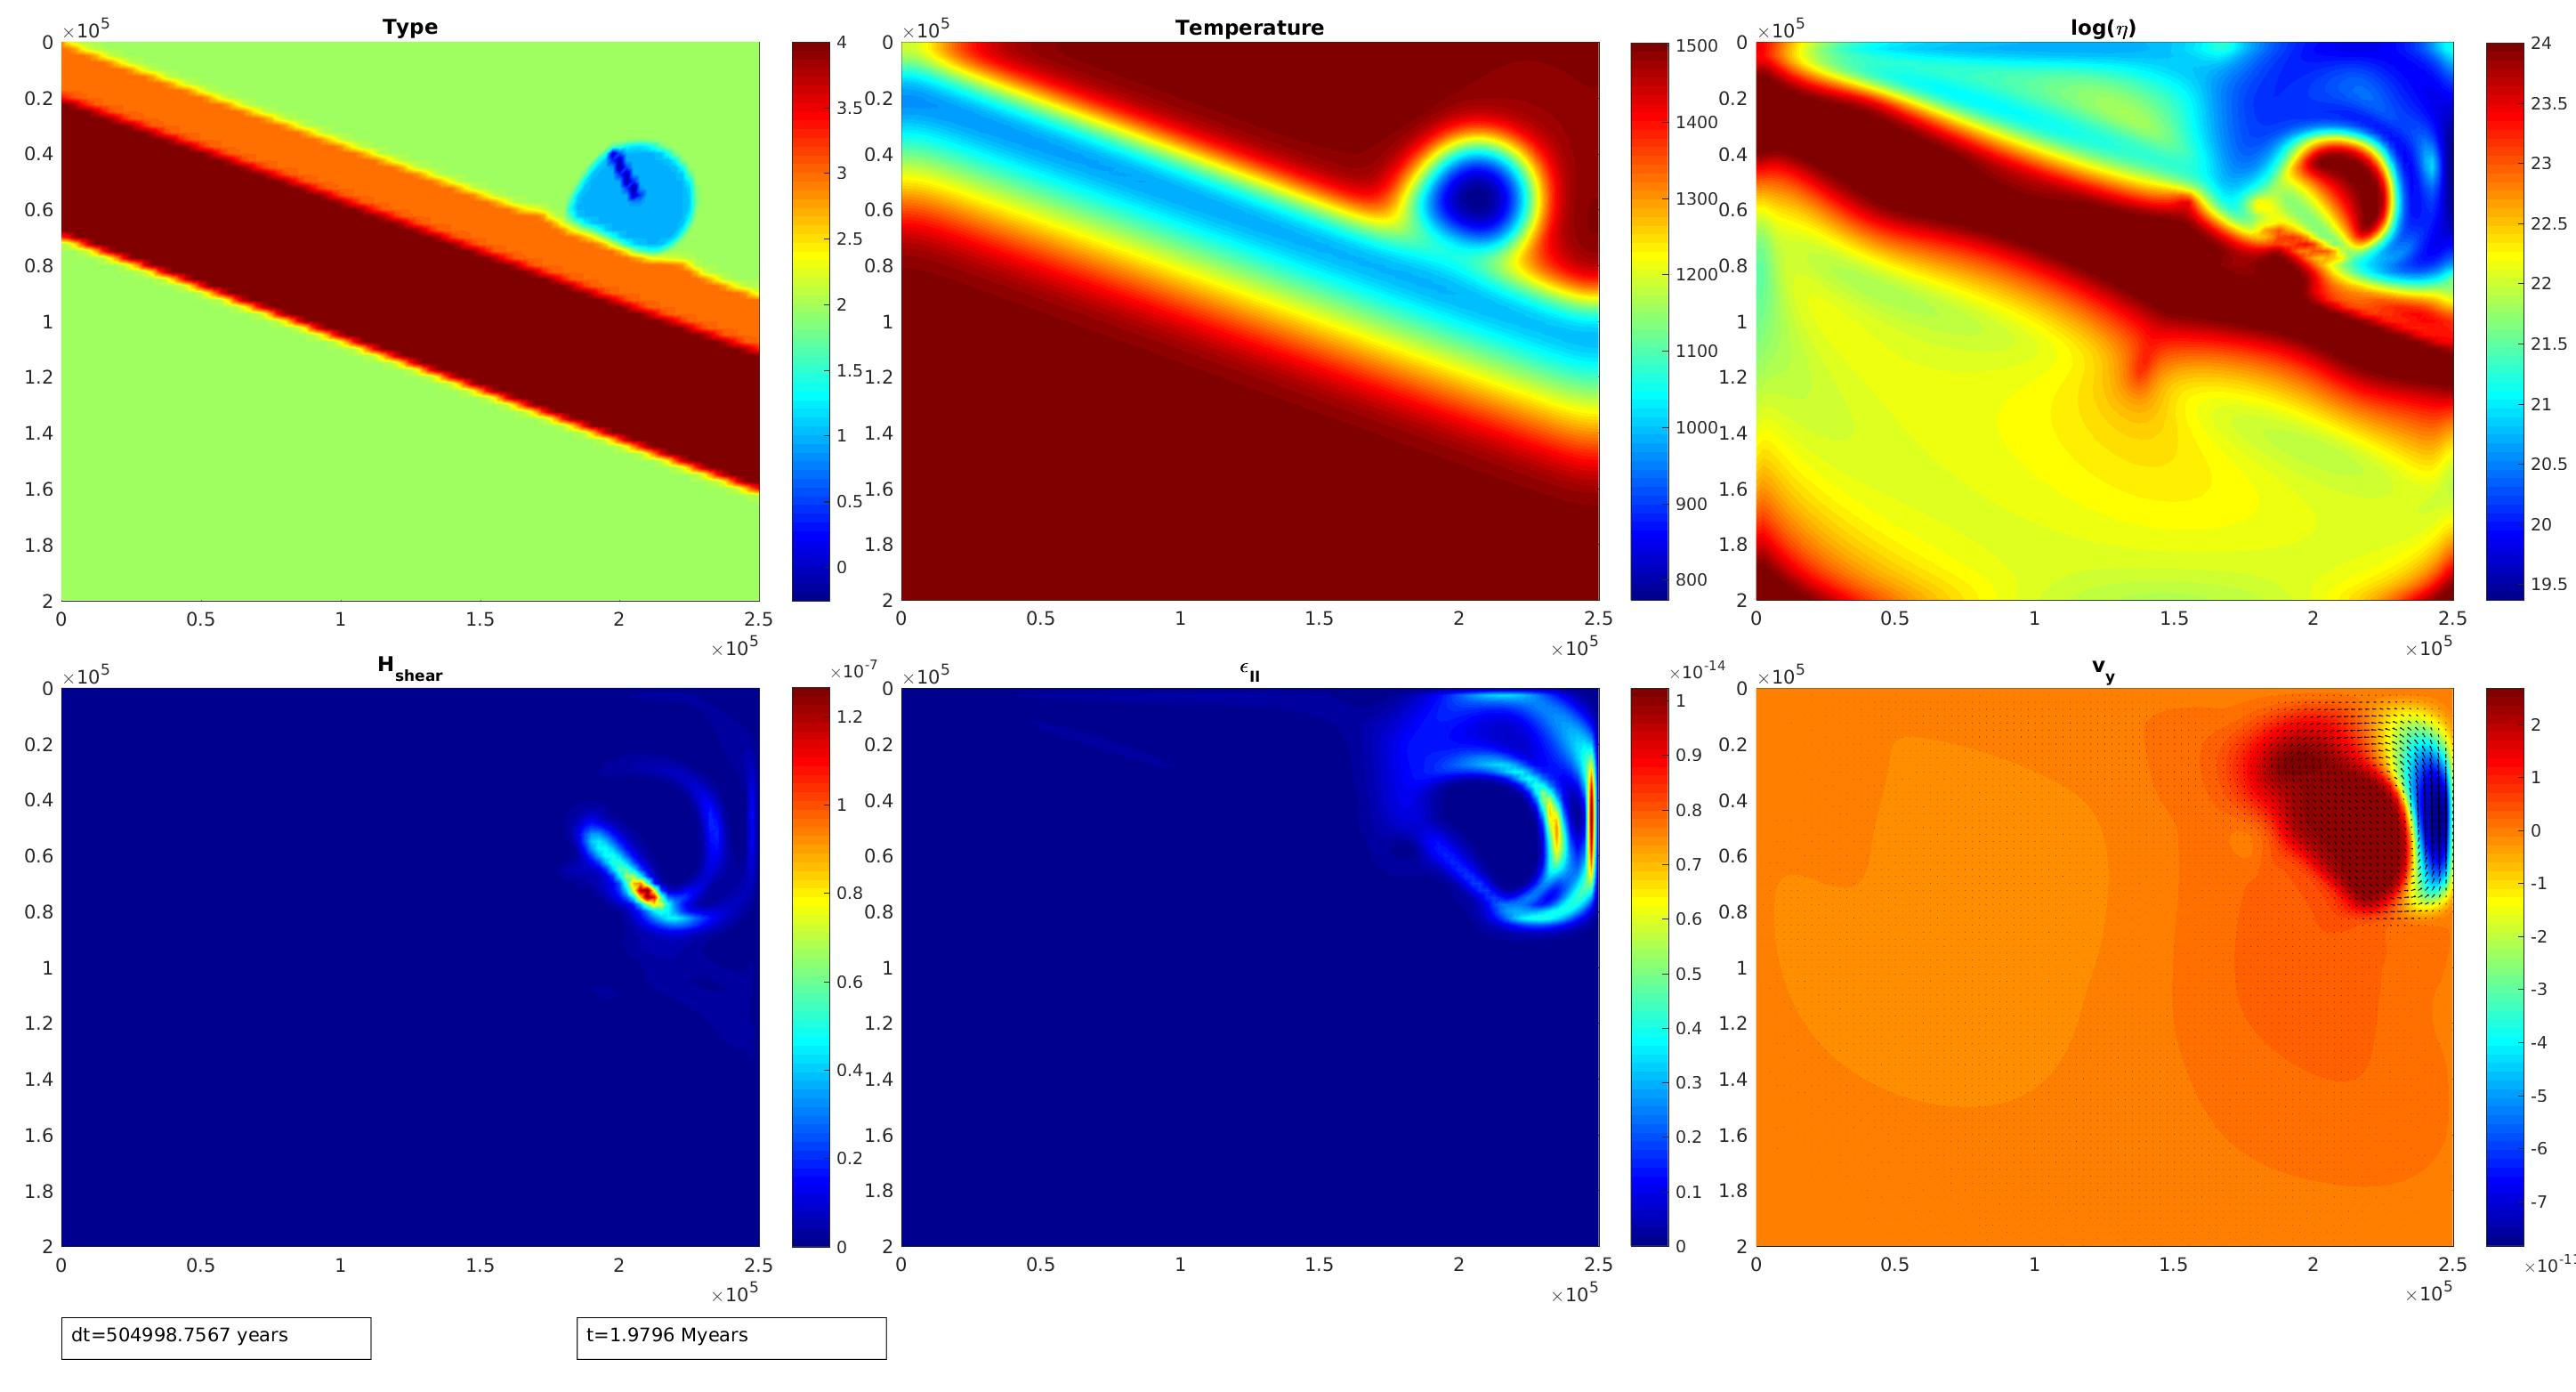
\includegraphics[width=1.0\textwidth]{./Snapshots/ref/Subductionzonewithblob51posrefslab20s2e7s2e7r20.jpg}
\end{minipage}
\caption{2 million years later in scenario 20 degrees}
\label{fig:2m20}
\end{figure}
\begin{figure}
\begin{minipage}[t]{1.0\textwidth}
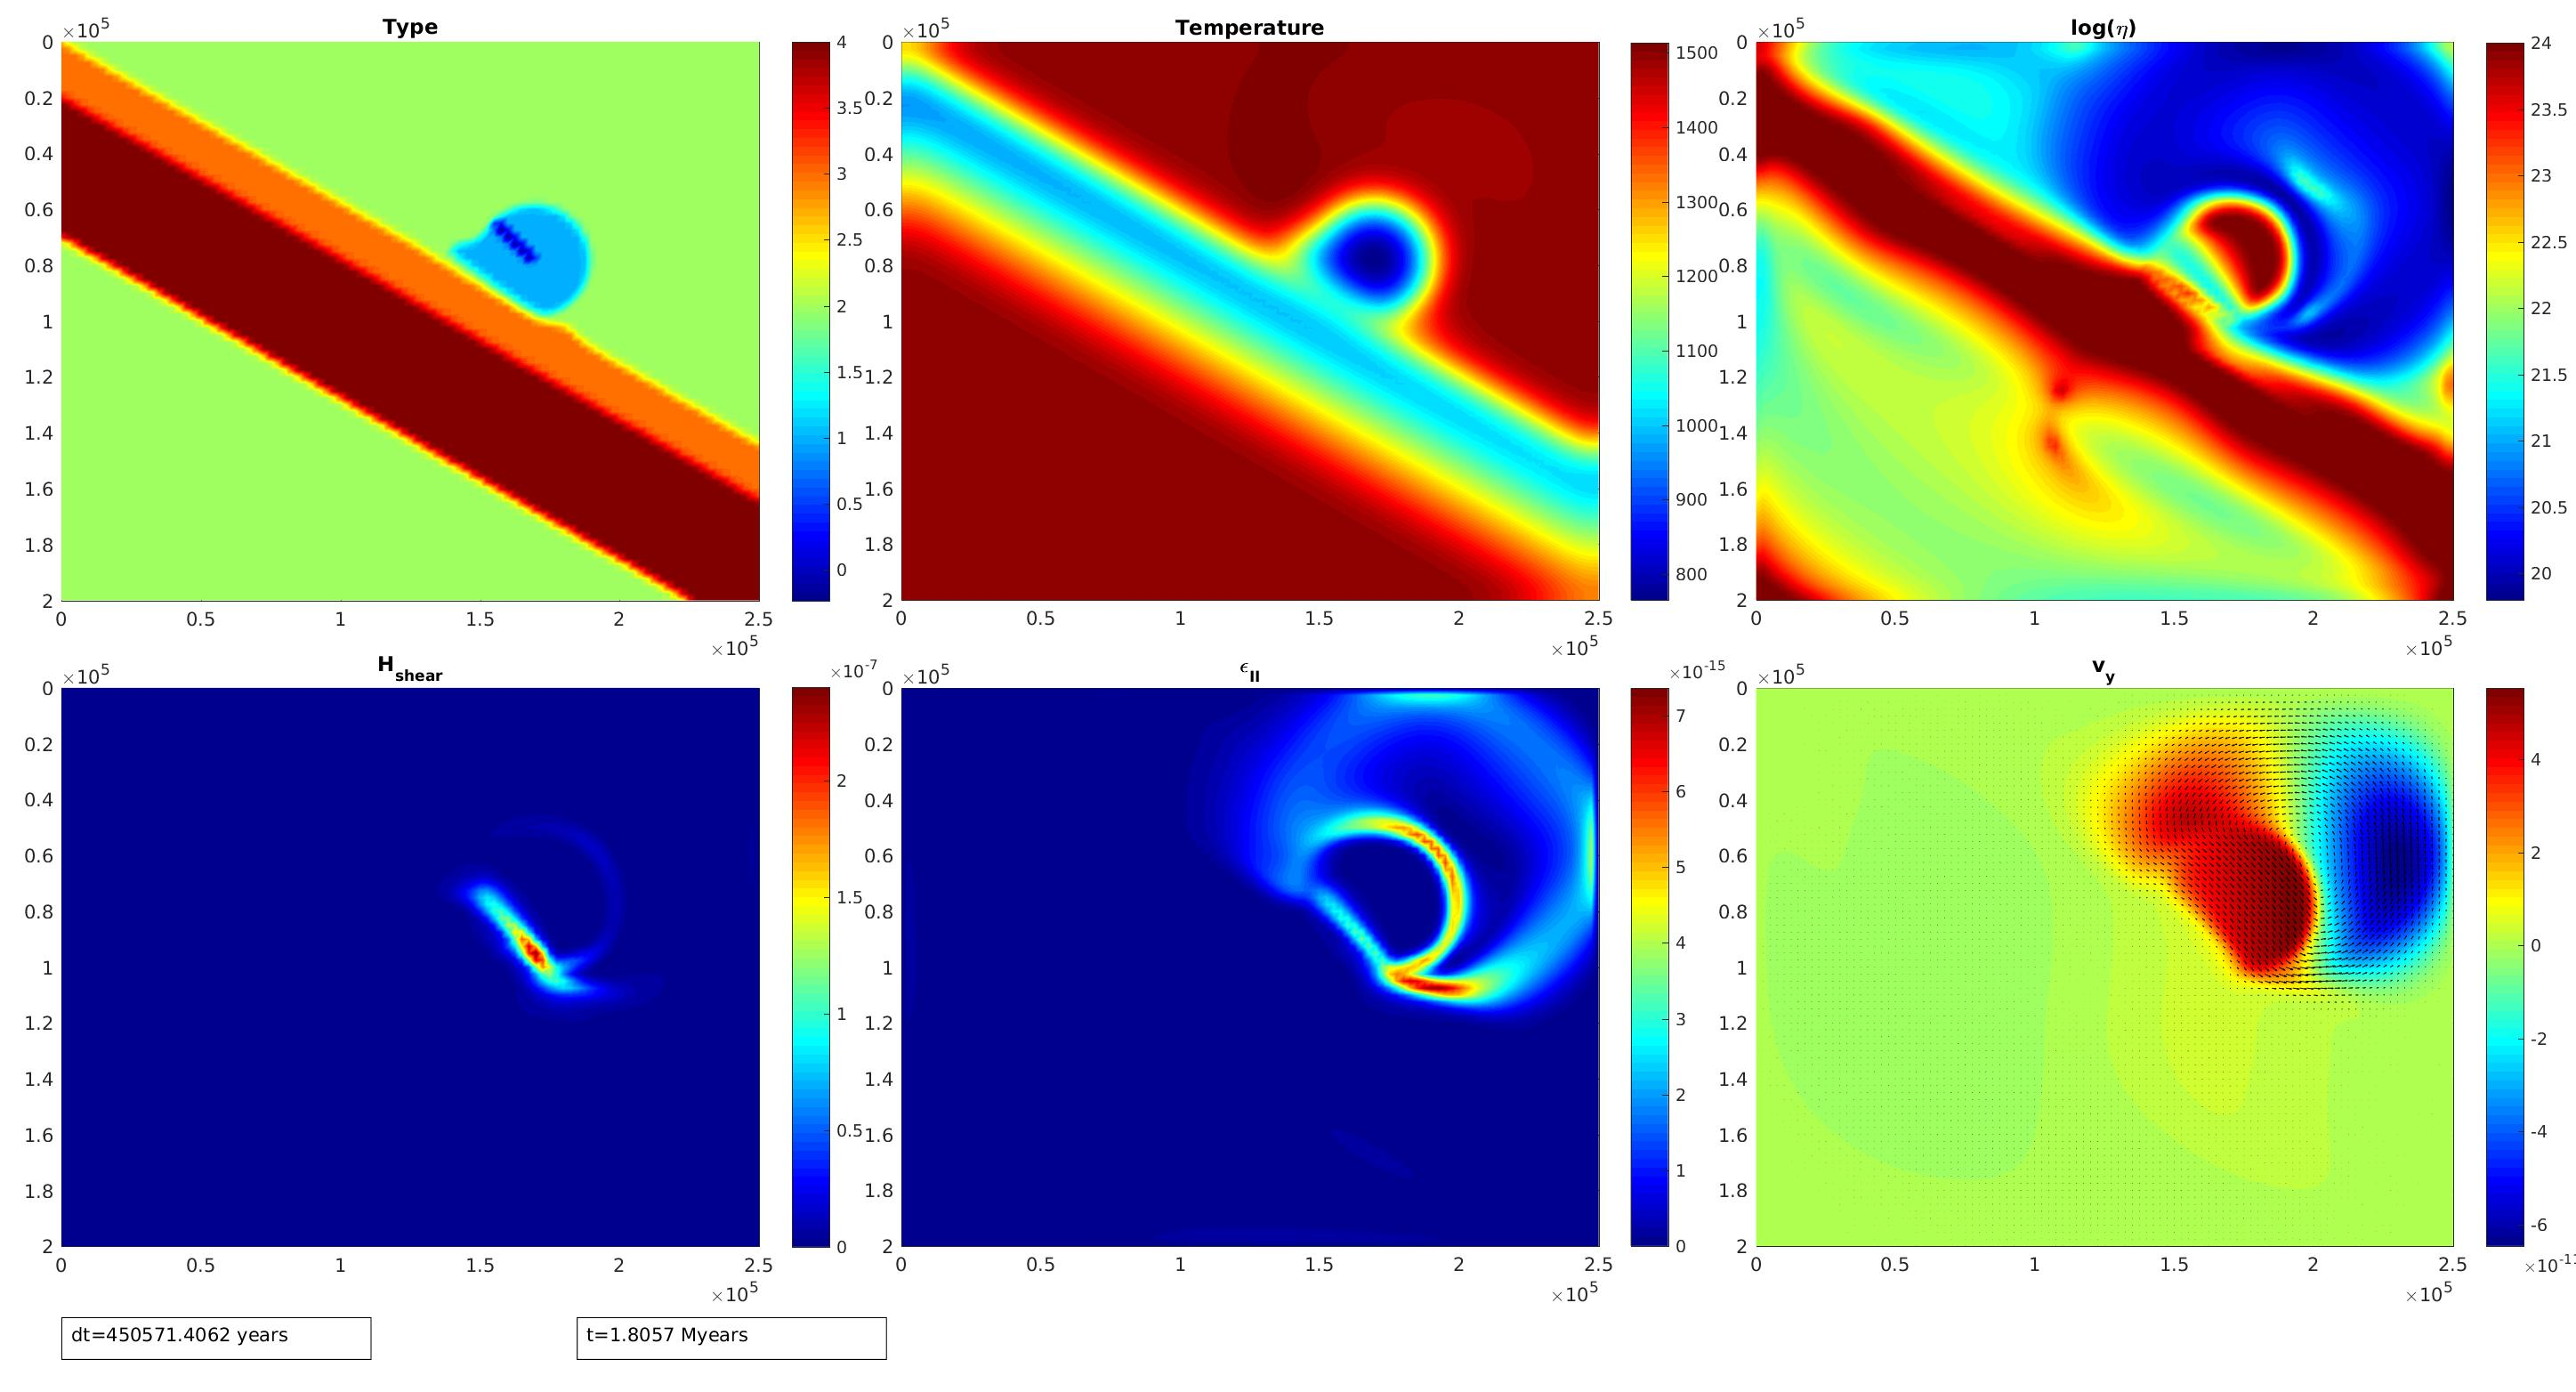
\includegraphics[width=1.0\textwidth]{./Snapshots/ref/Subductionzonewithblob63posrefslab30s2e7s2e7r20.jpg}
\end{minipage}
\caption{2 million years later in scenario 30 degrees}
\label{fig:2m30}
\end{figure}
\begin{figure}
\begin{minipage}[t]{1.0\textwidth}
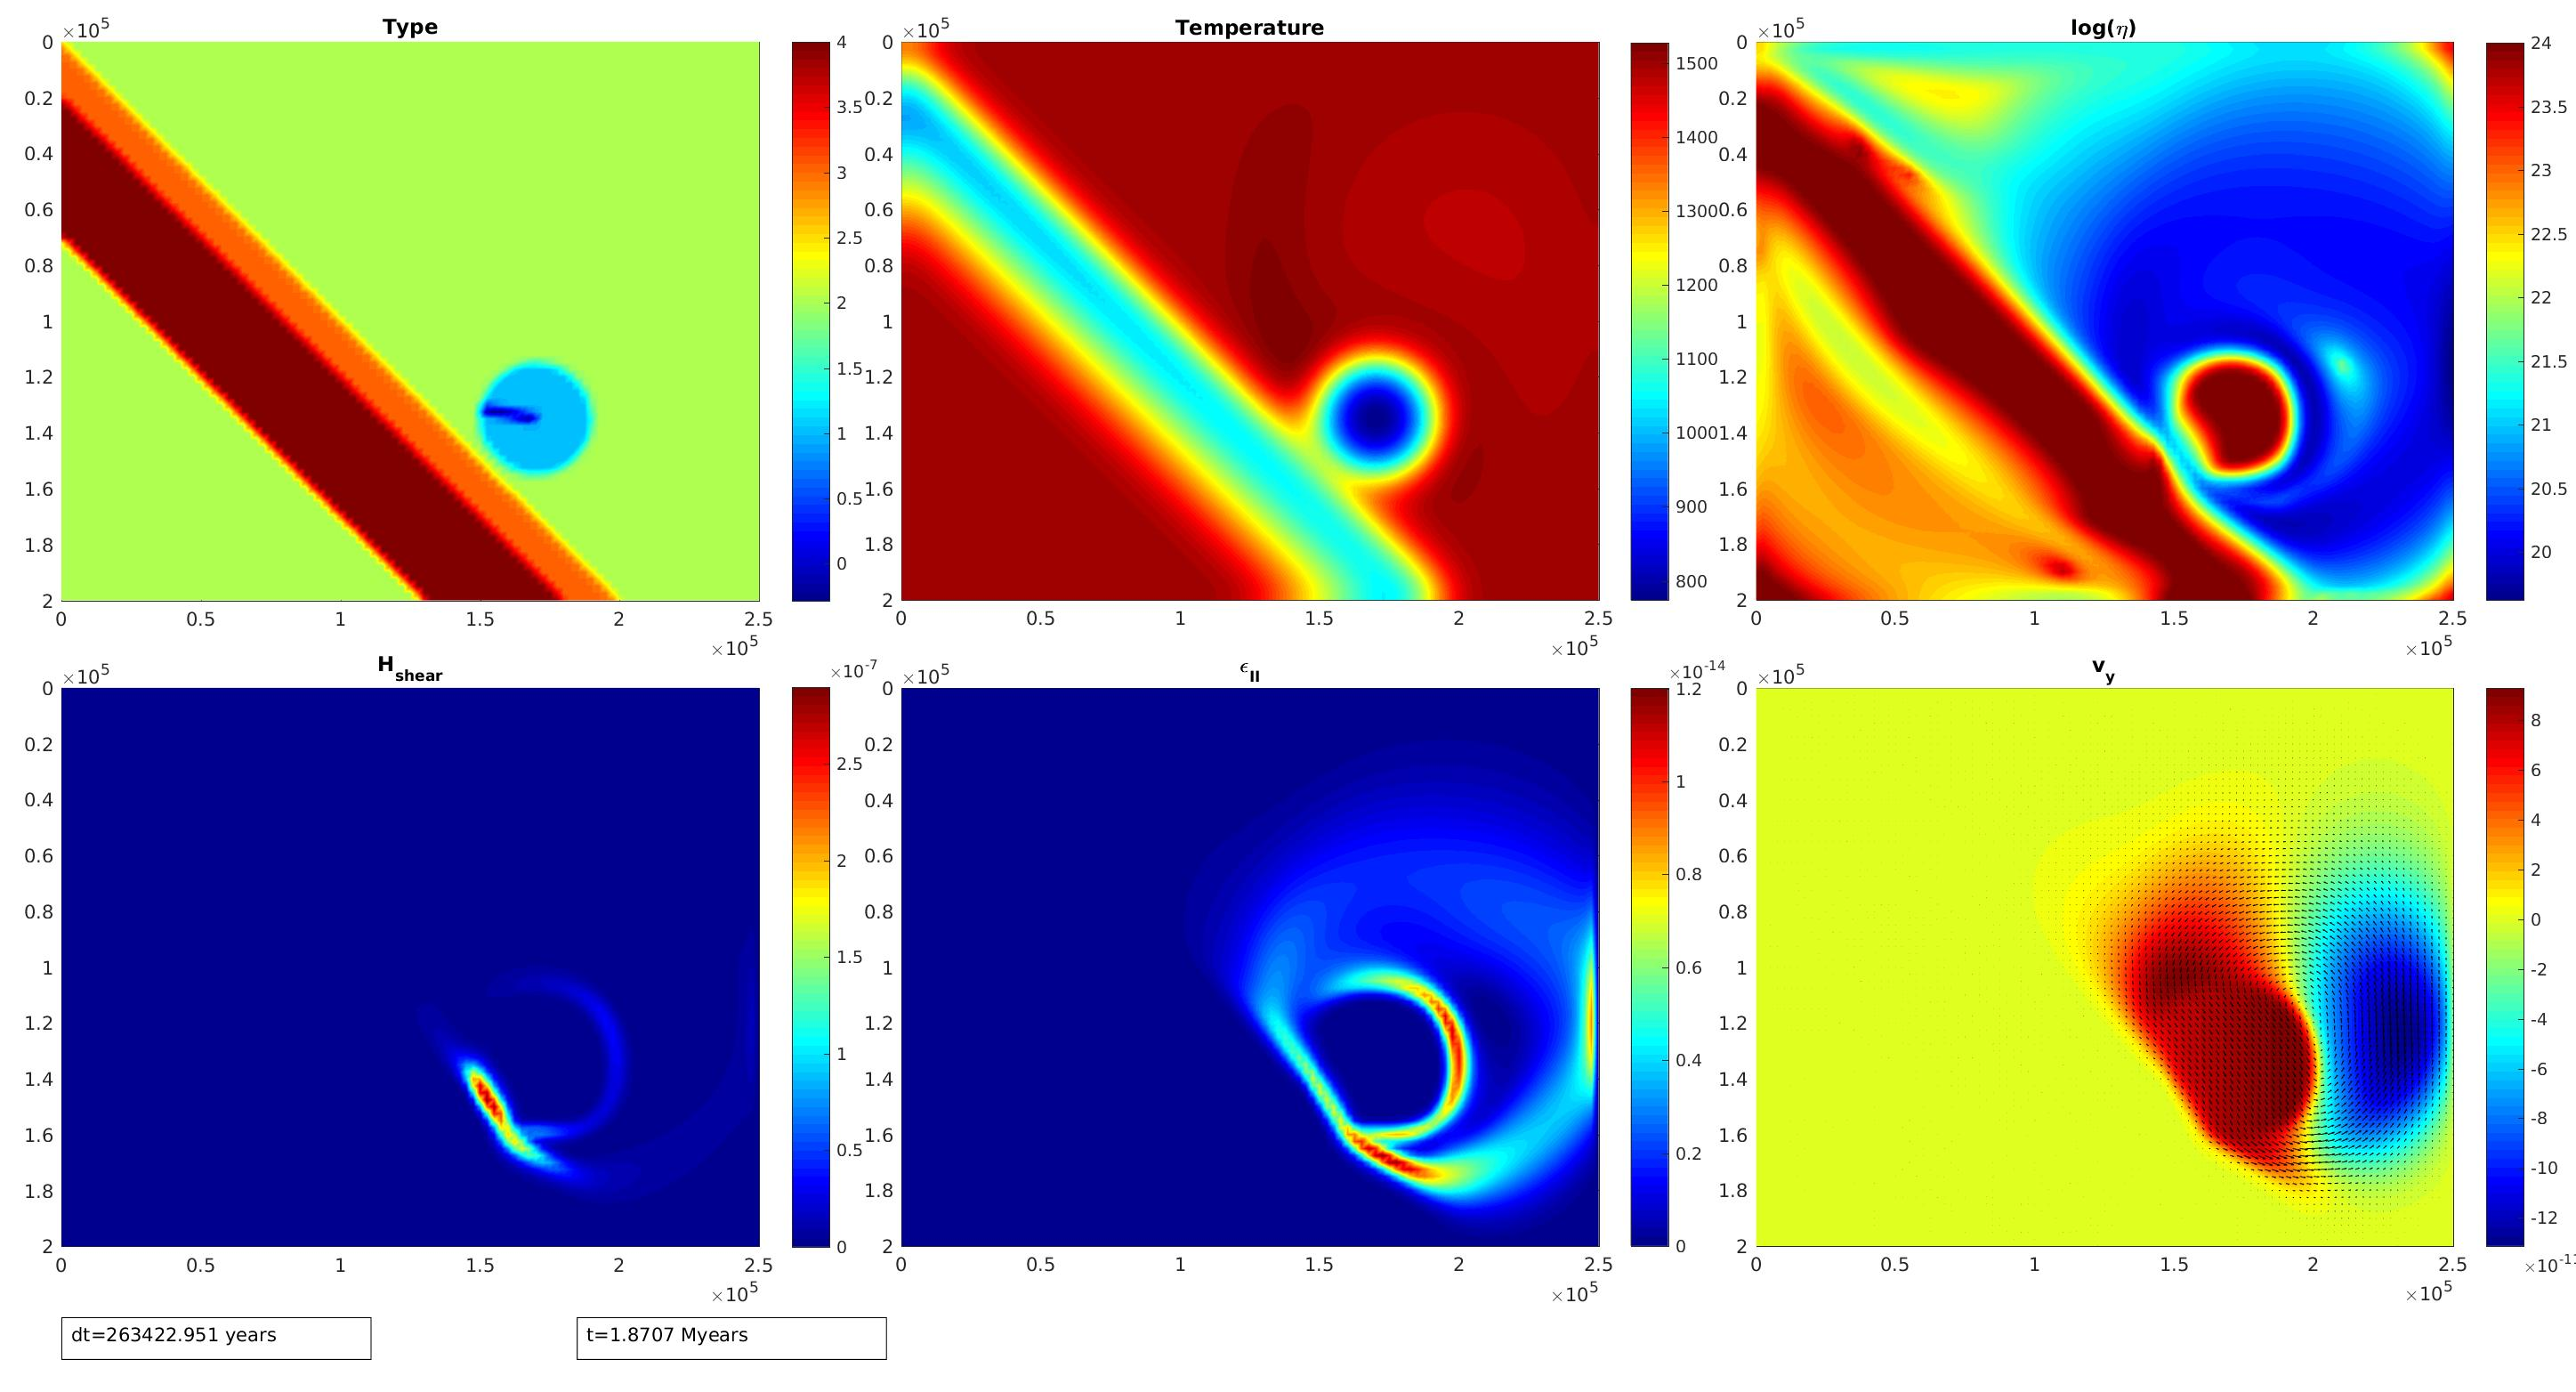
\includegraphics[width=1.0\textwidth]{./Snapshots/ref/Subductionzonewithblob92posrefslab45s2e7s2e7r20.jpg}
\end{minipage}
\caption{2 million years later in scenario 45 degrees}
\label{fig:2m45}
\end{figure}
\begin{figure}[!ht]
\begin{minipage}[t]{1.0\textwidth}
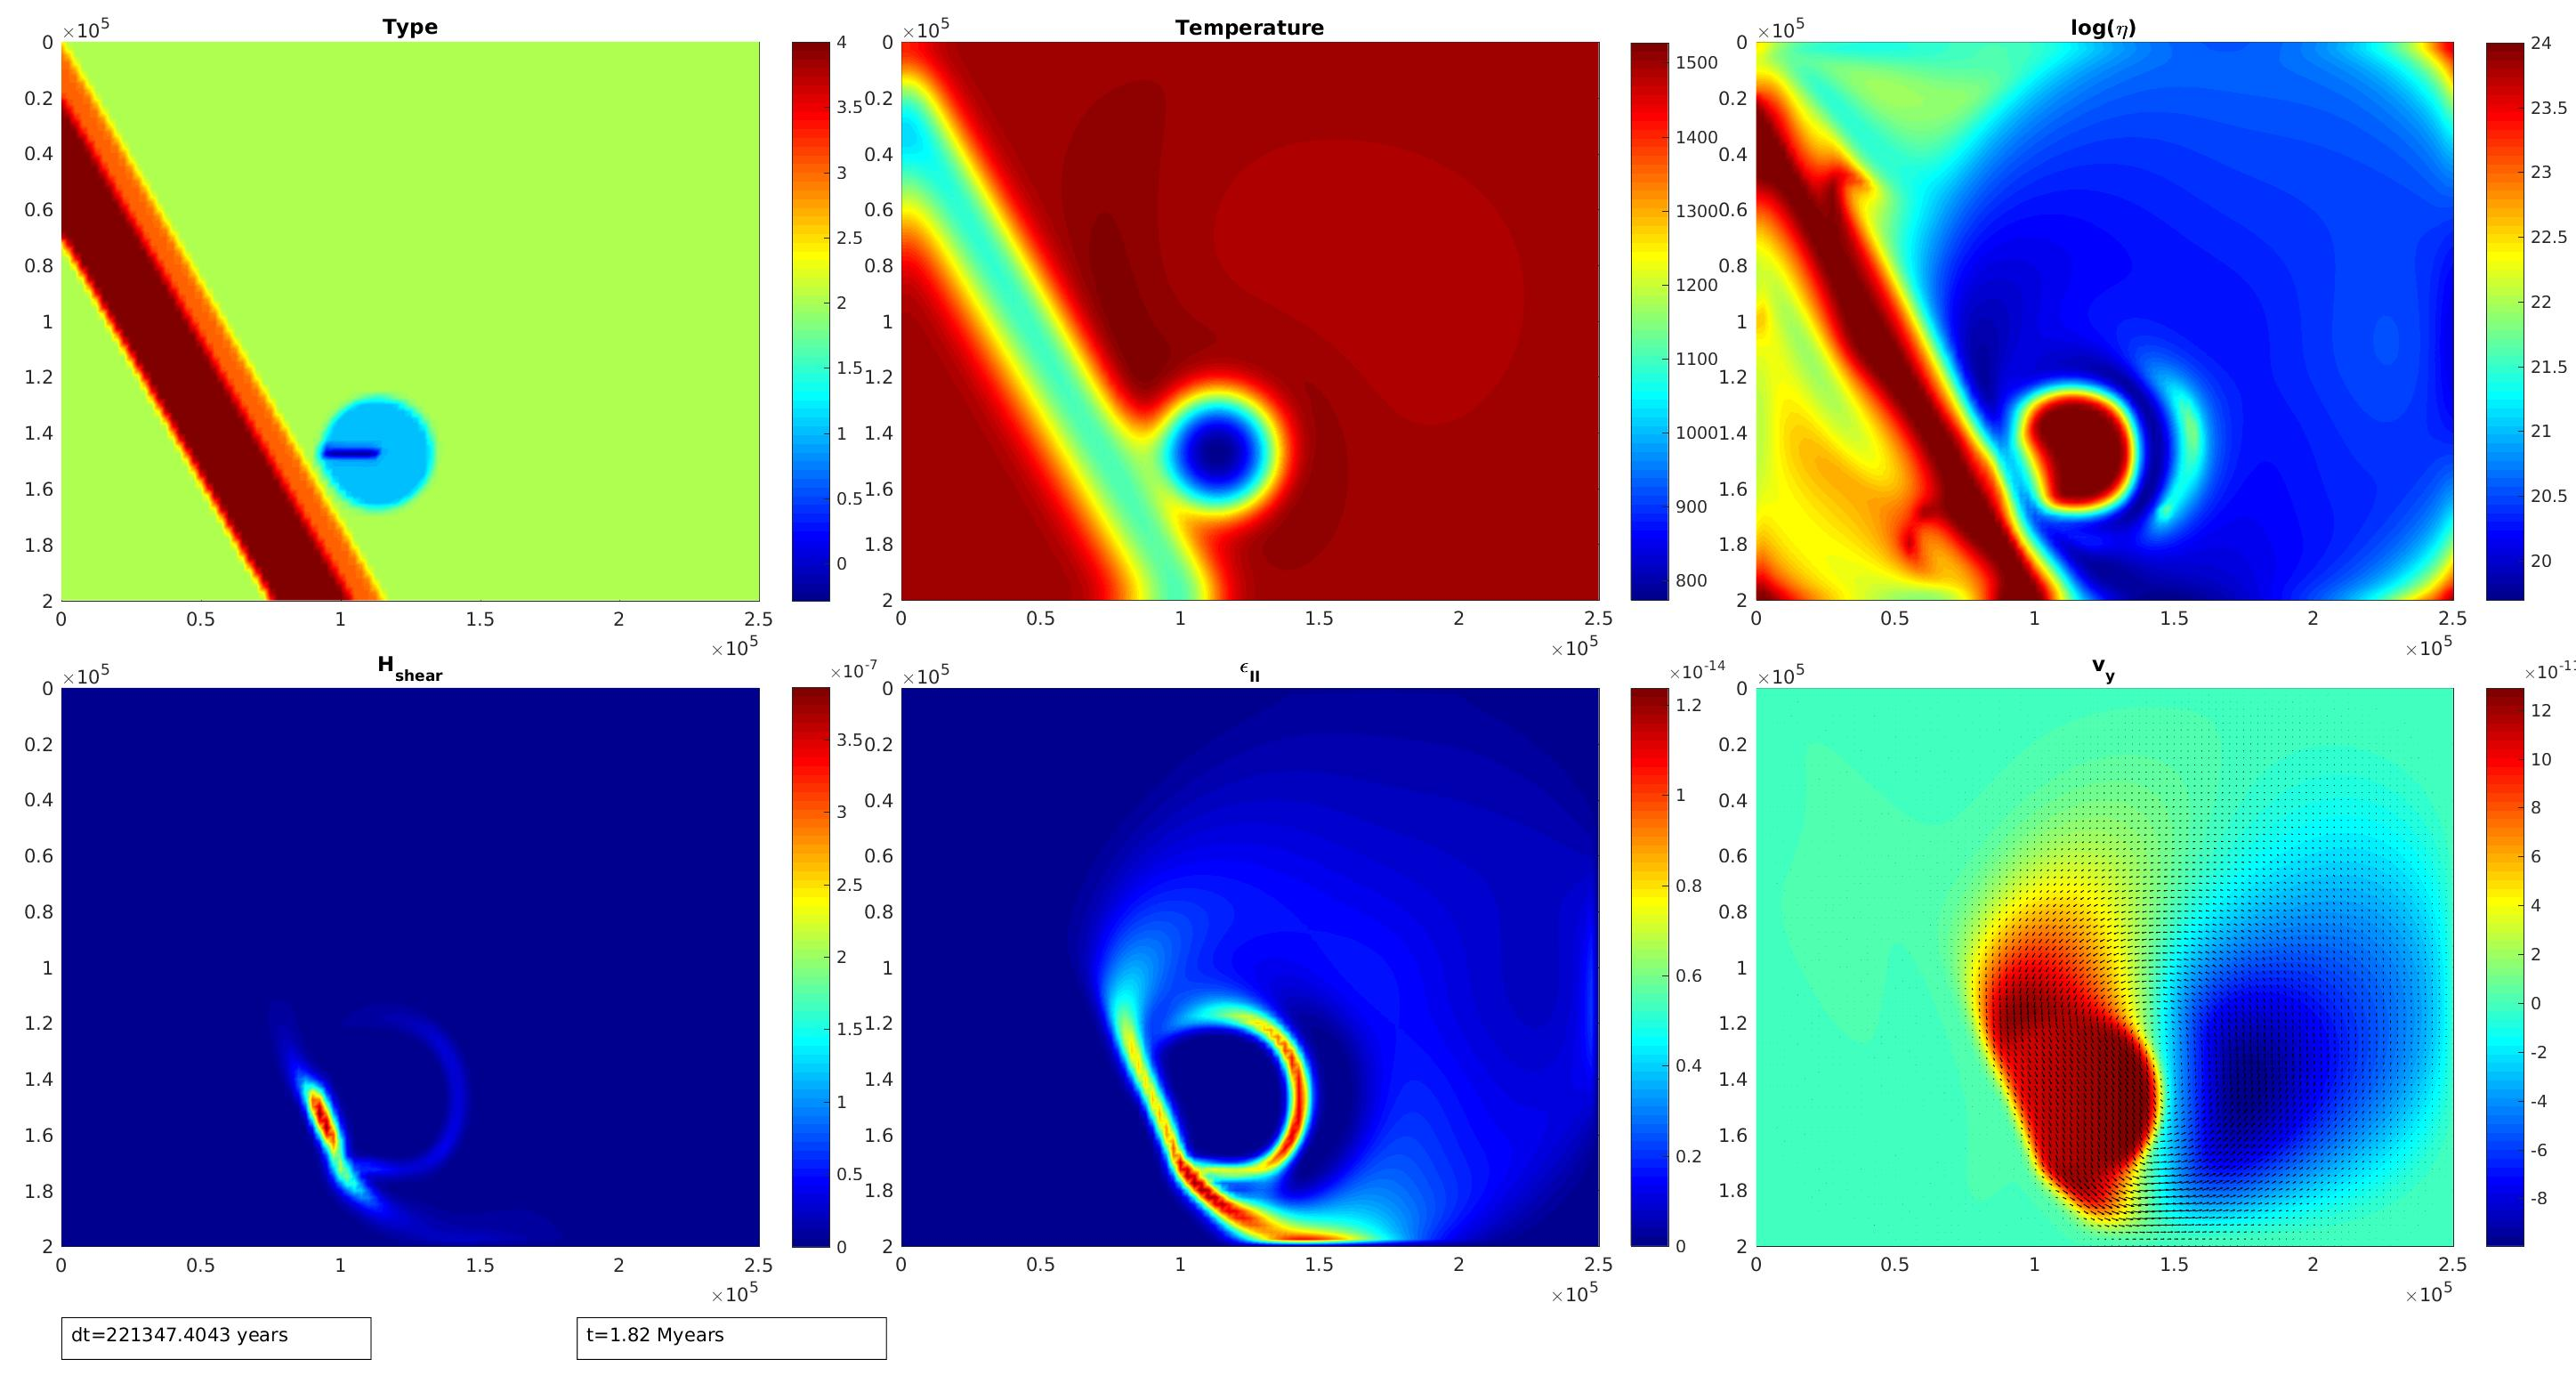
\includegraphics[width=1.0\textwidth]{./Snapshots/ref/Subductionzonewithblob101posrefslab60s2e7s2e7r20.jpg}
\end{minipage}
\caption{2 million years later in scenario 60 degrees}
\label{fig:2m60}
\end{figure}
\begin{figure}
\begin{minipage}[t]{1.0\textwidth}
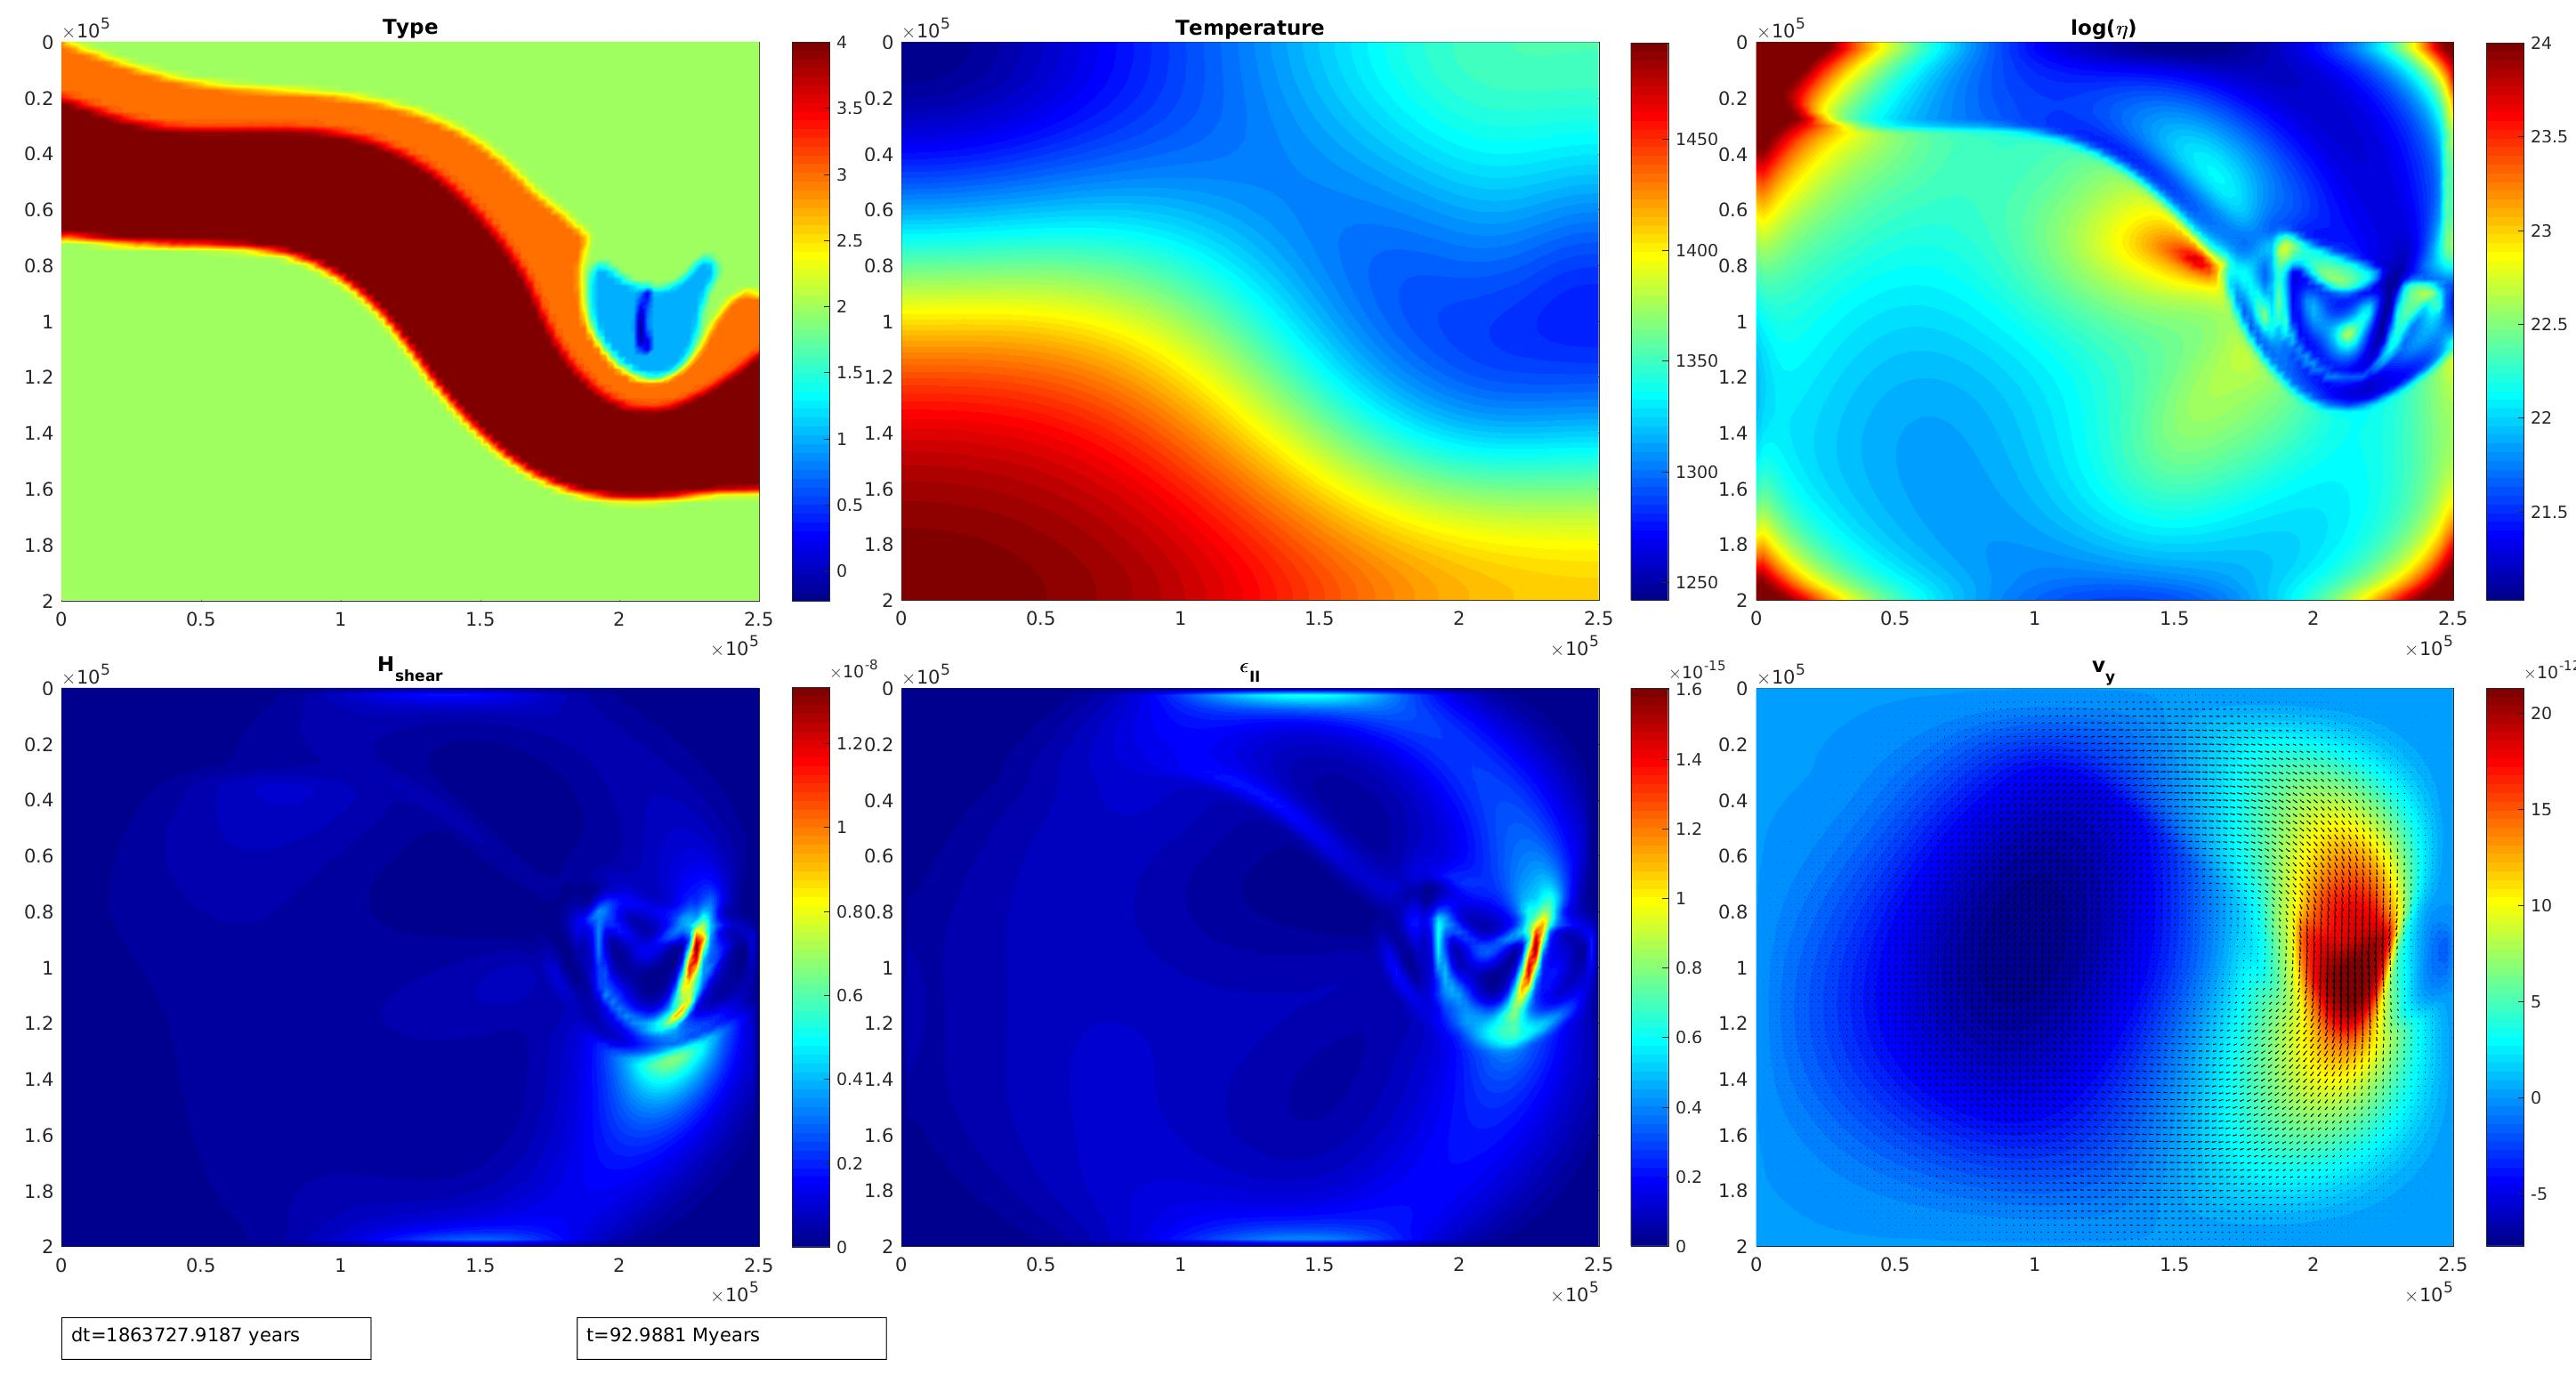
\includegraphics[width=1.0\textwidth]{./Snapshots/ref/Subductionzonewithblob100posrefslab20s2e7s2e7r20.jpg}
\end{minipage}
\caption{100 timesteps later in scenario 20 degrees}
\label{fig:100t20}
\end{figure}
\begin{figure}
\begin{minipage}[t]{1.0\textwidth}
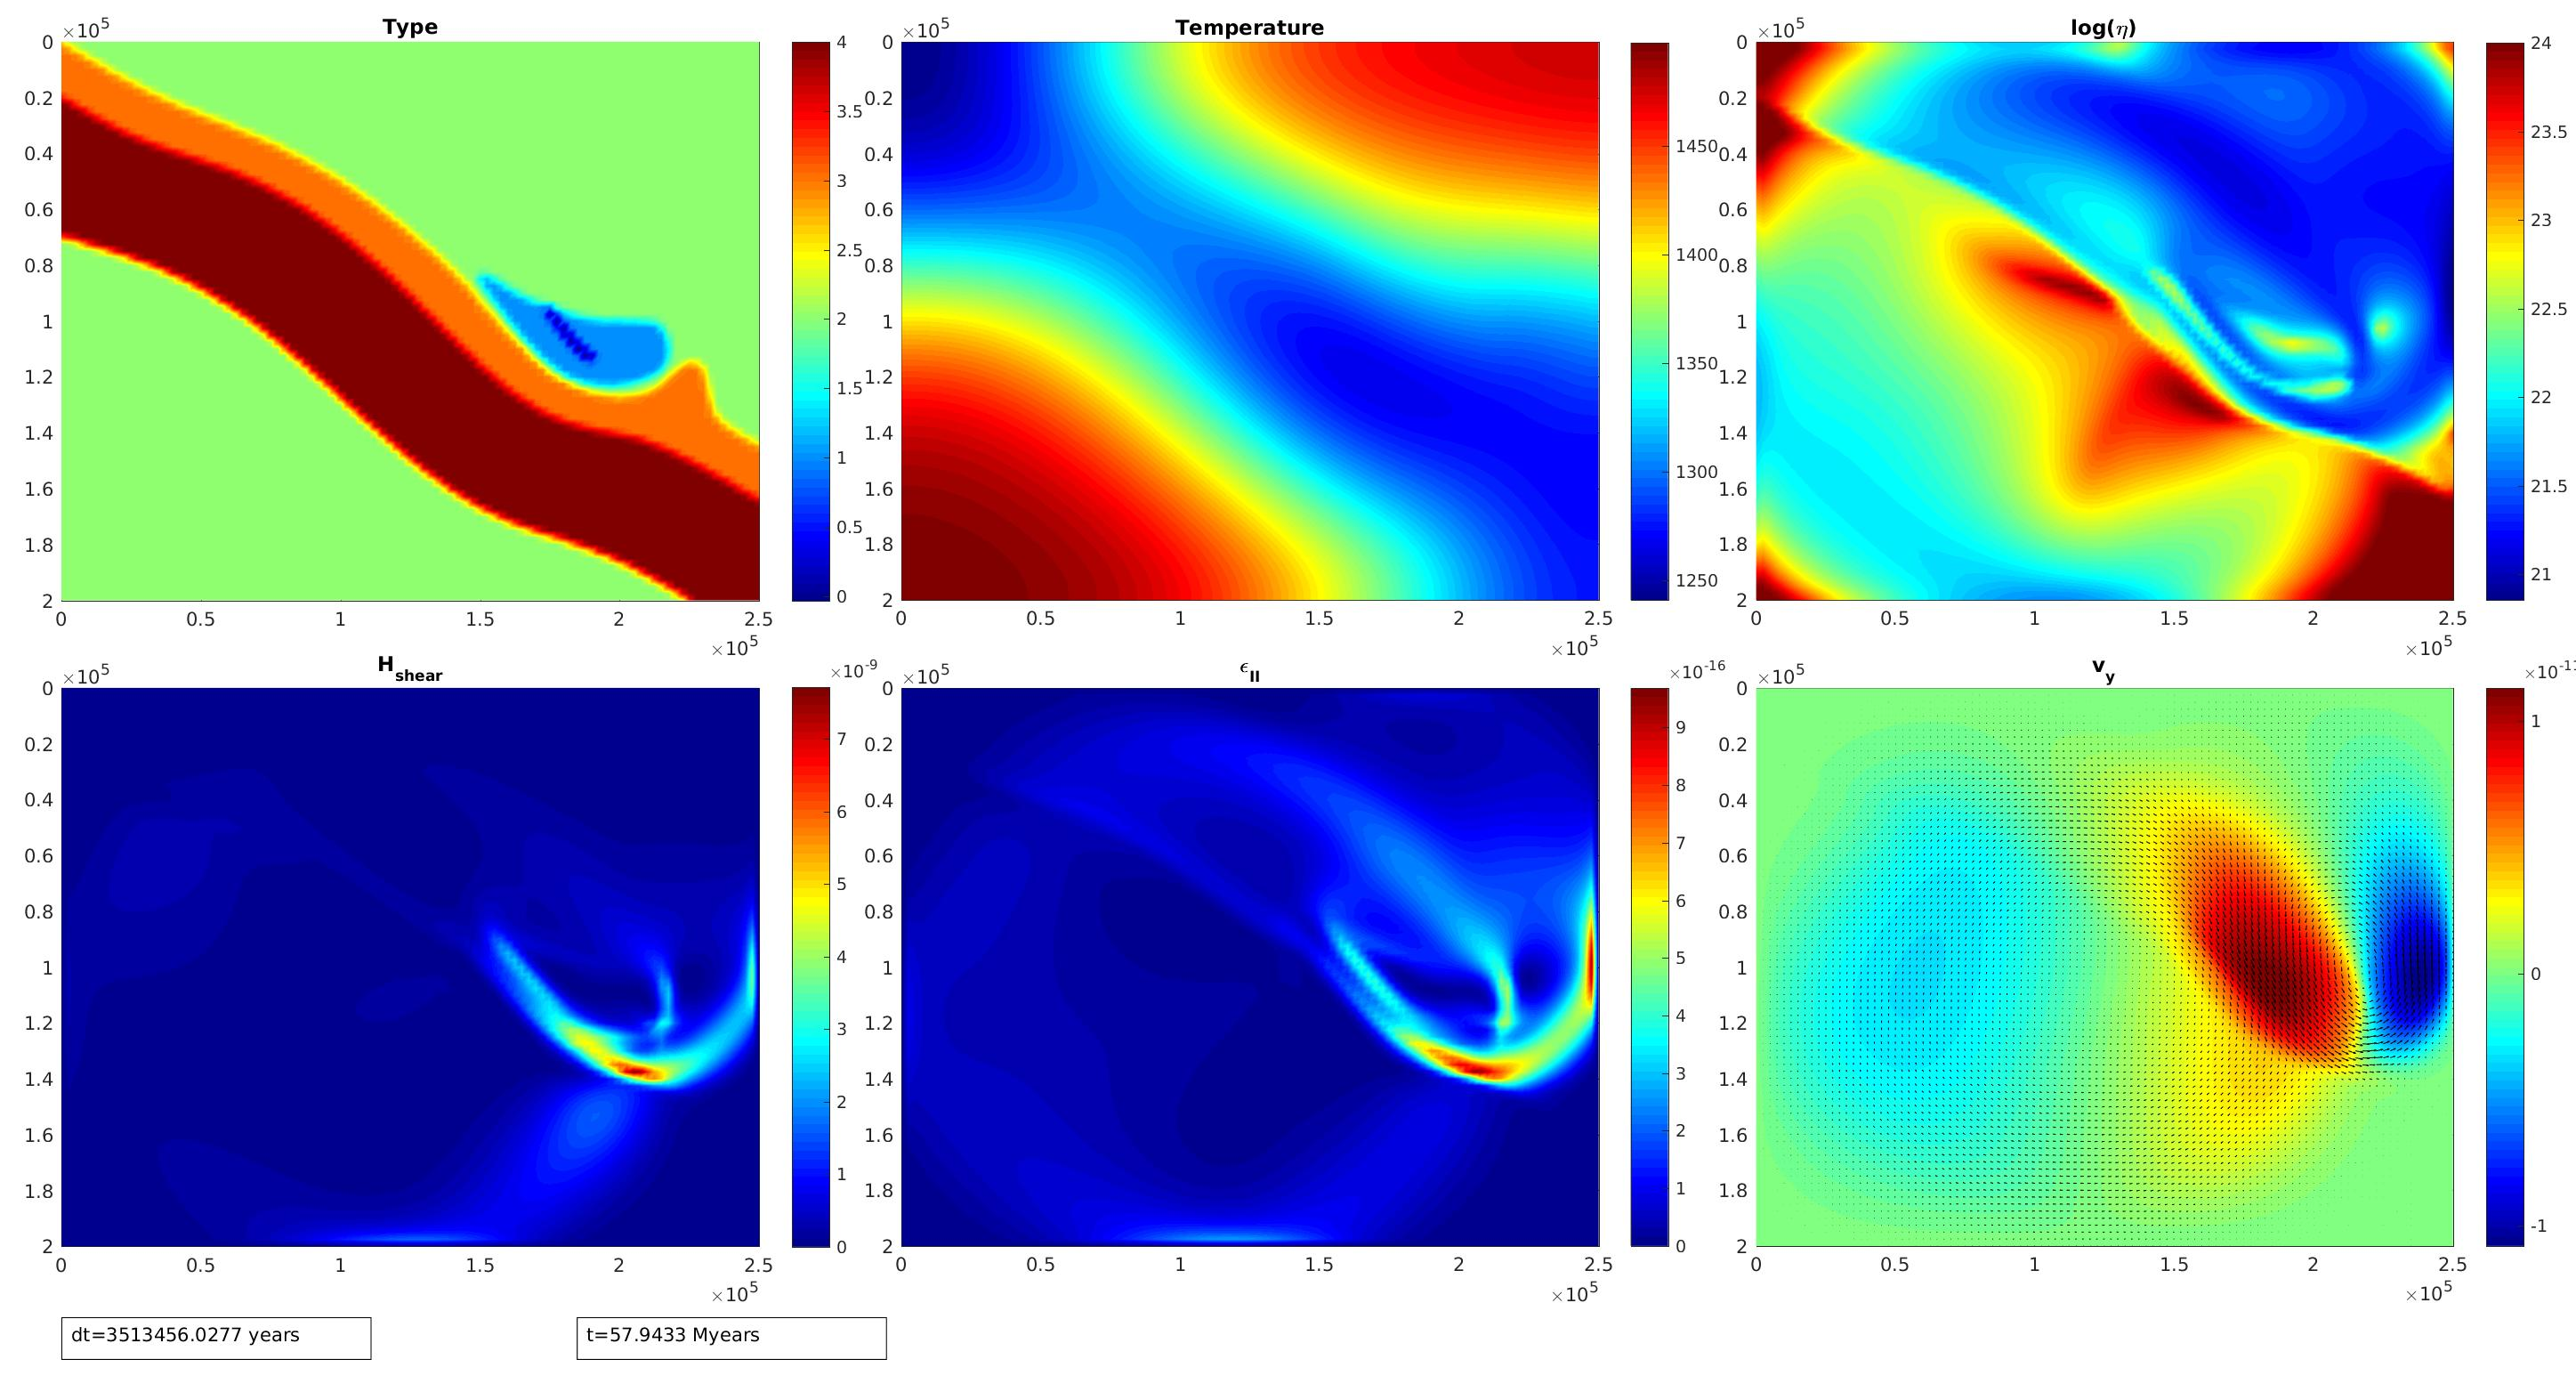
\includegraphics[width=1.0\textwidth]{./Snapshots/ref/Subductionzonewithblob100posrefslab30s2e7s2e7r20.jpg}
\end{minipage}
\caption{100 timesteps later in scenario 30 degrees}
\label{fig:100t30}
\end{figure}
\begin{figure}
\begin{minipage}[t]{1.0\textwidth}
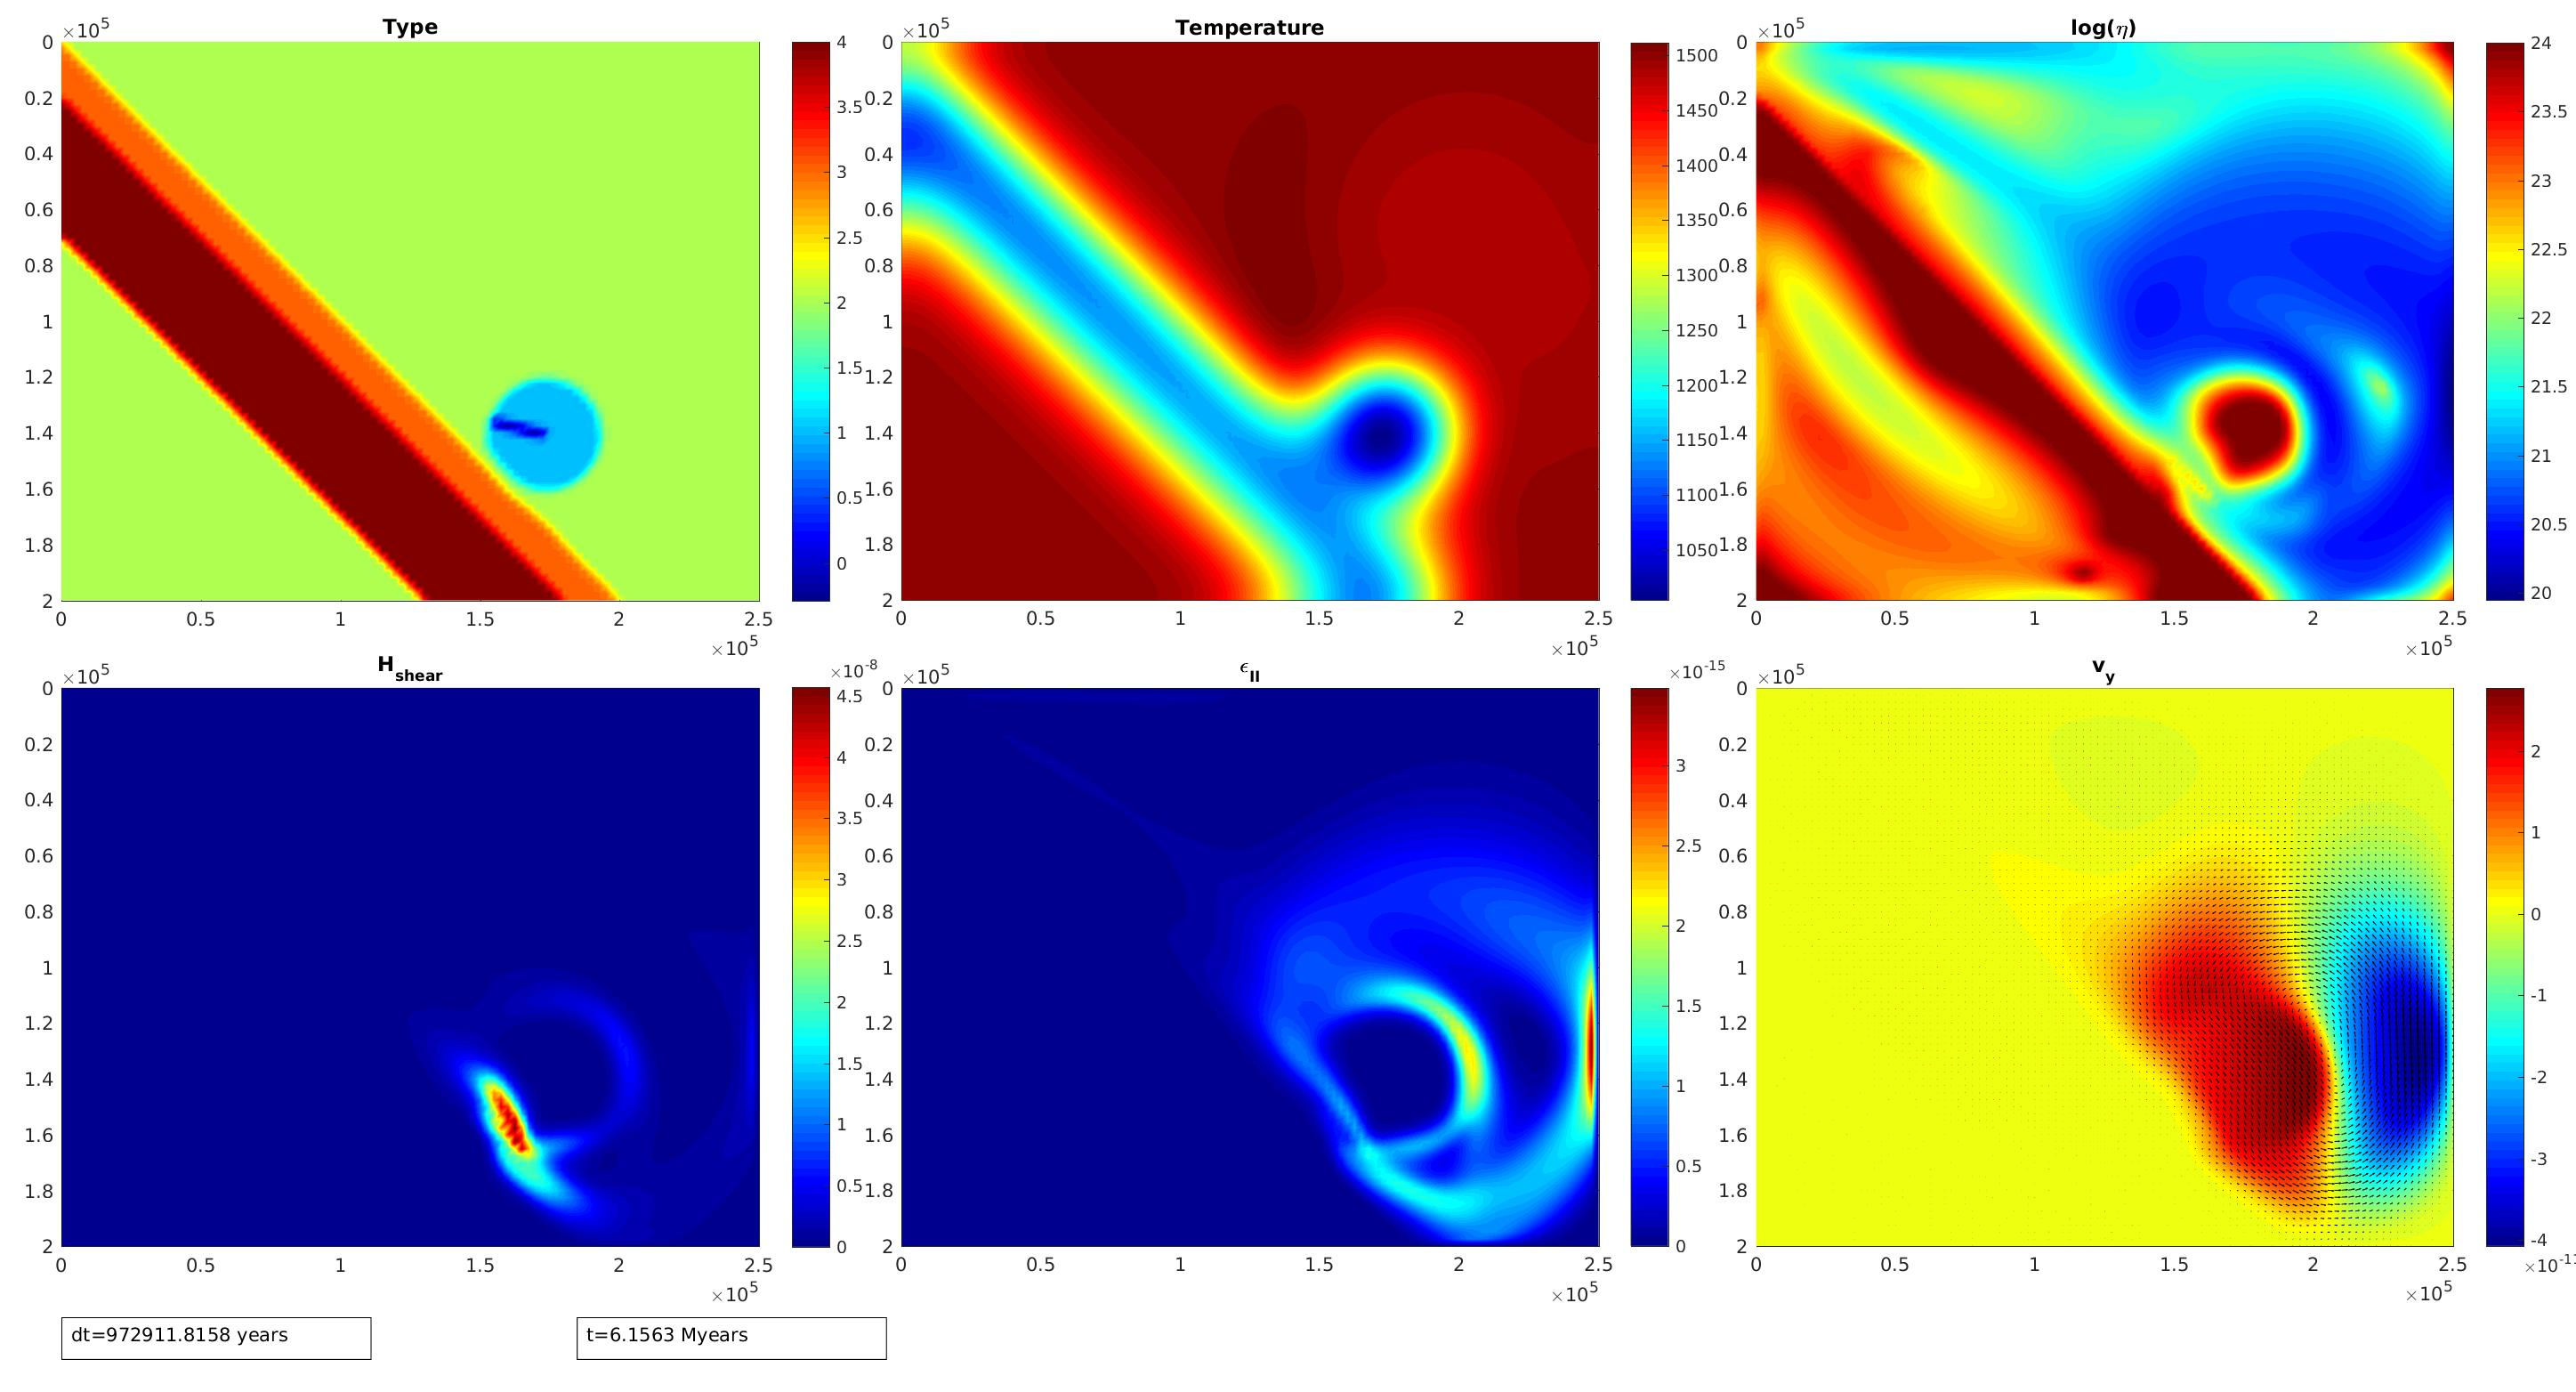
\includegraphics[width=1.0\textwidth]{./Snapshots/ref/Subductionzonewithblob100posrefslab45s2e7s2e7r20.jpg}
\end{minipage}
\caption{100 timesteps later in scenario 45 degrees}
\label{fig:100t45}
\end{figure}
\begin{figure}
\begin{minipage}[t]{1.0\textwidth}
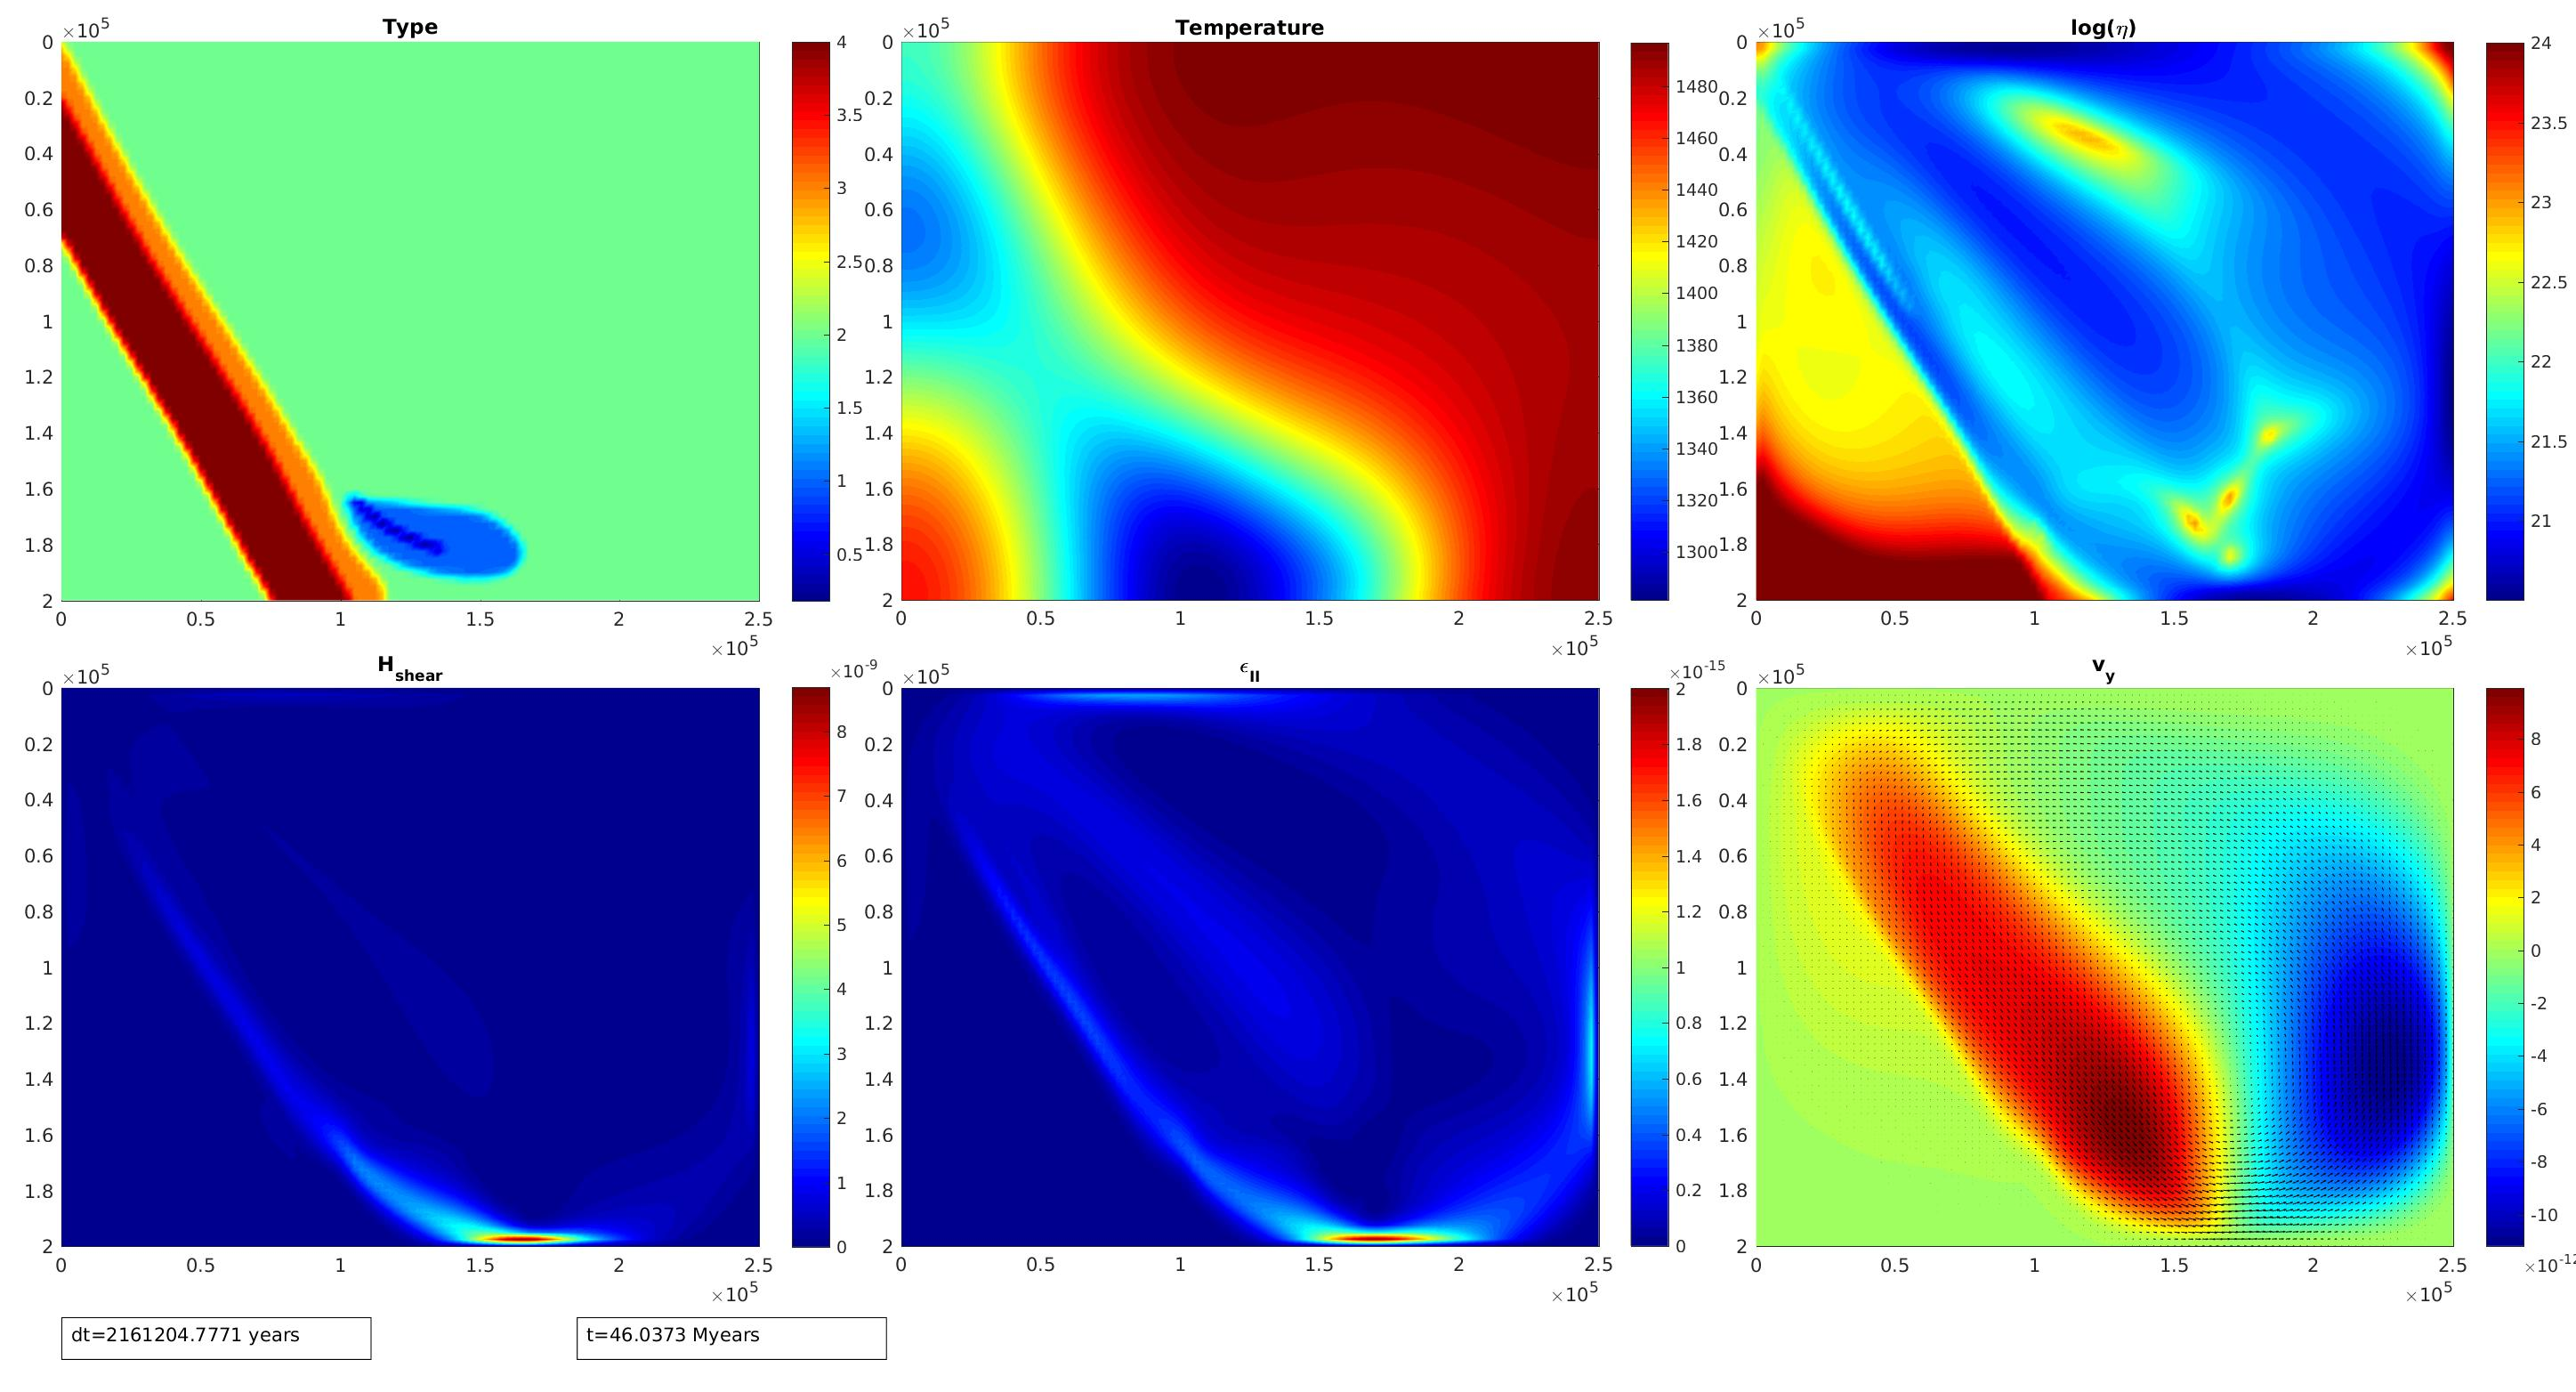
\includegraphics[width=1.0\textwidth]{./Snapshots/ref/Subductionzonewithblob150posrefslab60s2e7s2e7r20.jpg}
\end{minipage}
\caption{150 timesteps later in scenario 60 degrees}
\label{fig:150t60}
\end{figure}
\begin{figure}
\begin{minipage}[t]{1.0\textwidth}
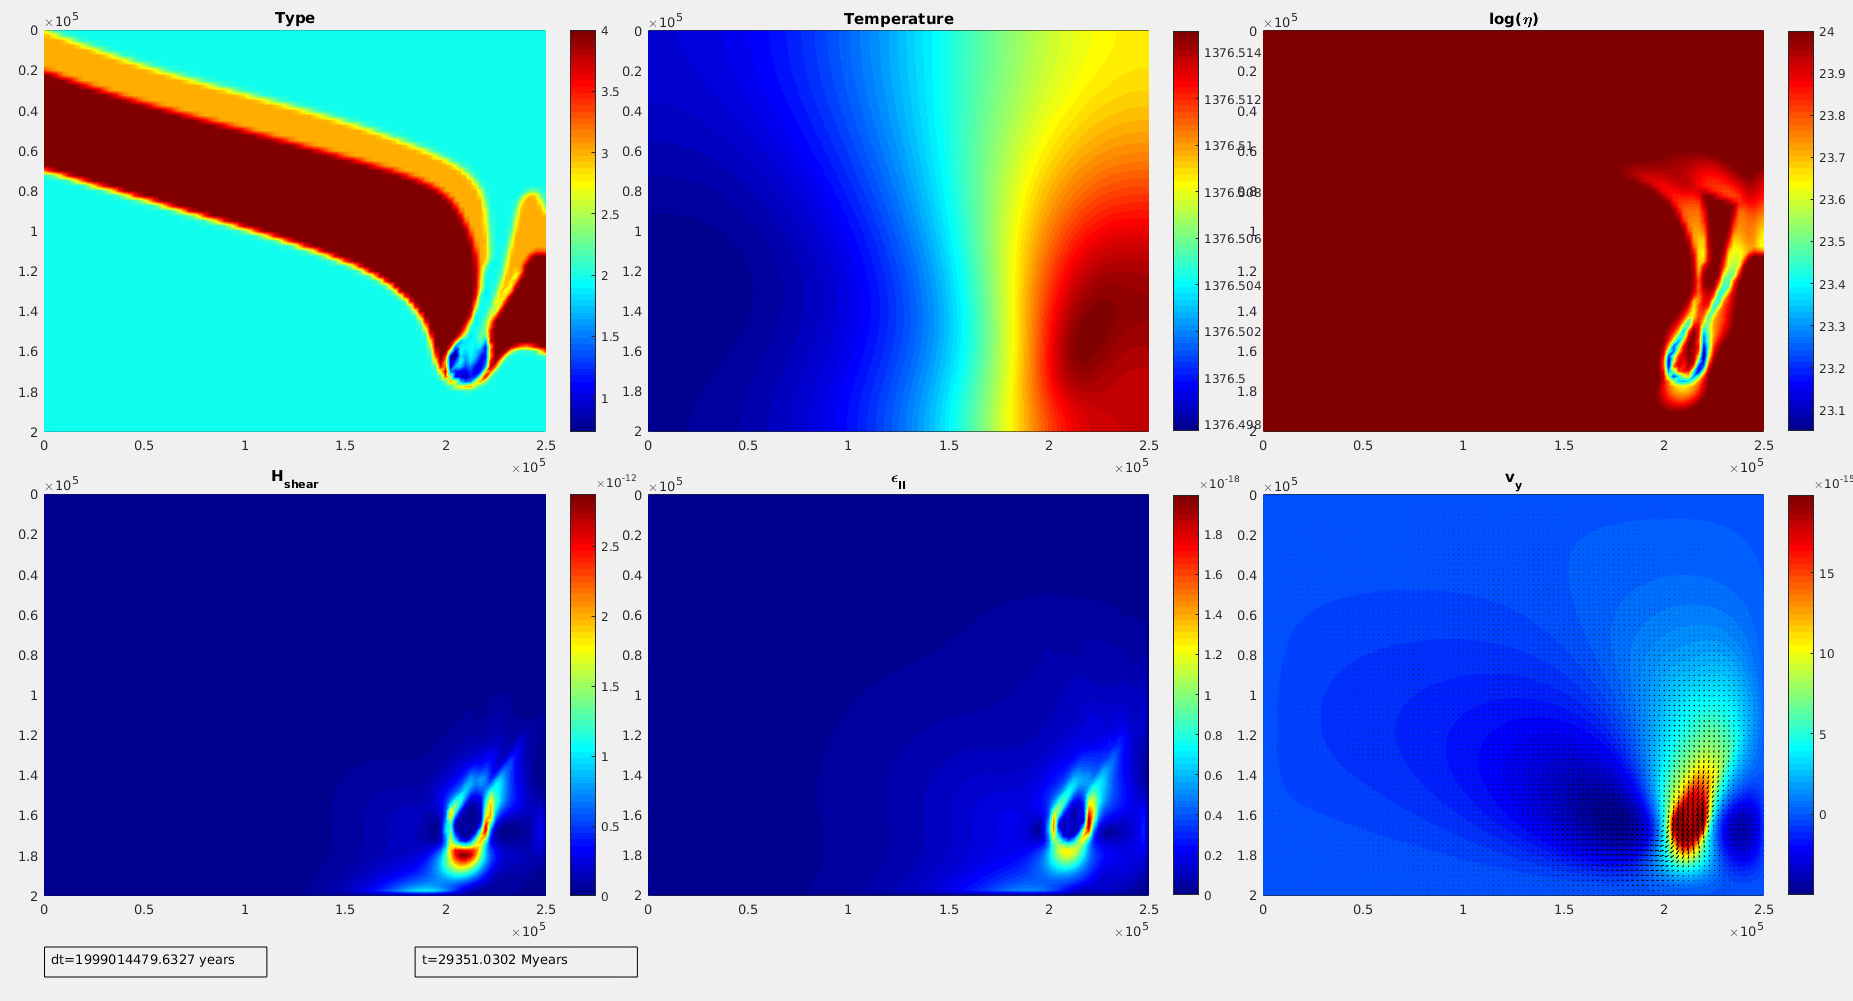
\includegraphics[width=1.0\textwidth]{./Snapshots/ref/Subductionzonewithblobposref150slab20s1e7r10.jpg}
\end{minipage}
\caption{150 timesteps later in scenario 20 degrees with radius 10km}
\label{fig:150t2010km}
\end{figure}
\begin{figure}
\begin{minipage}[t]{1.0\textwidth}
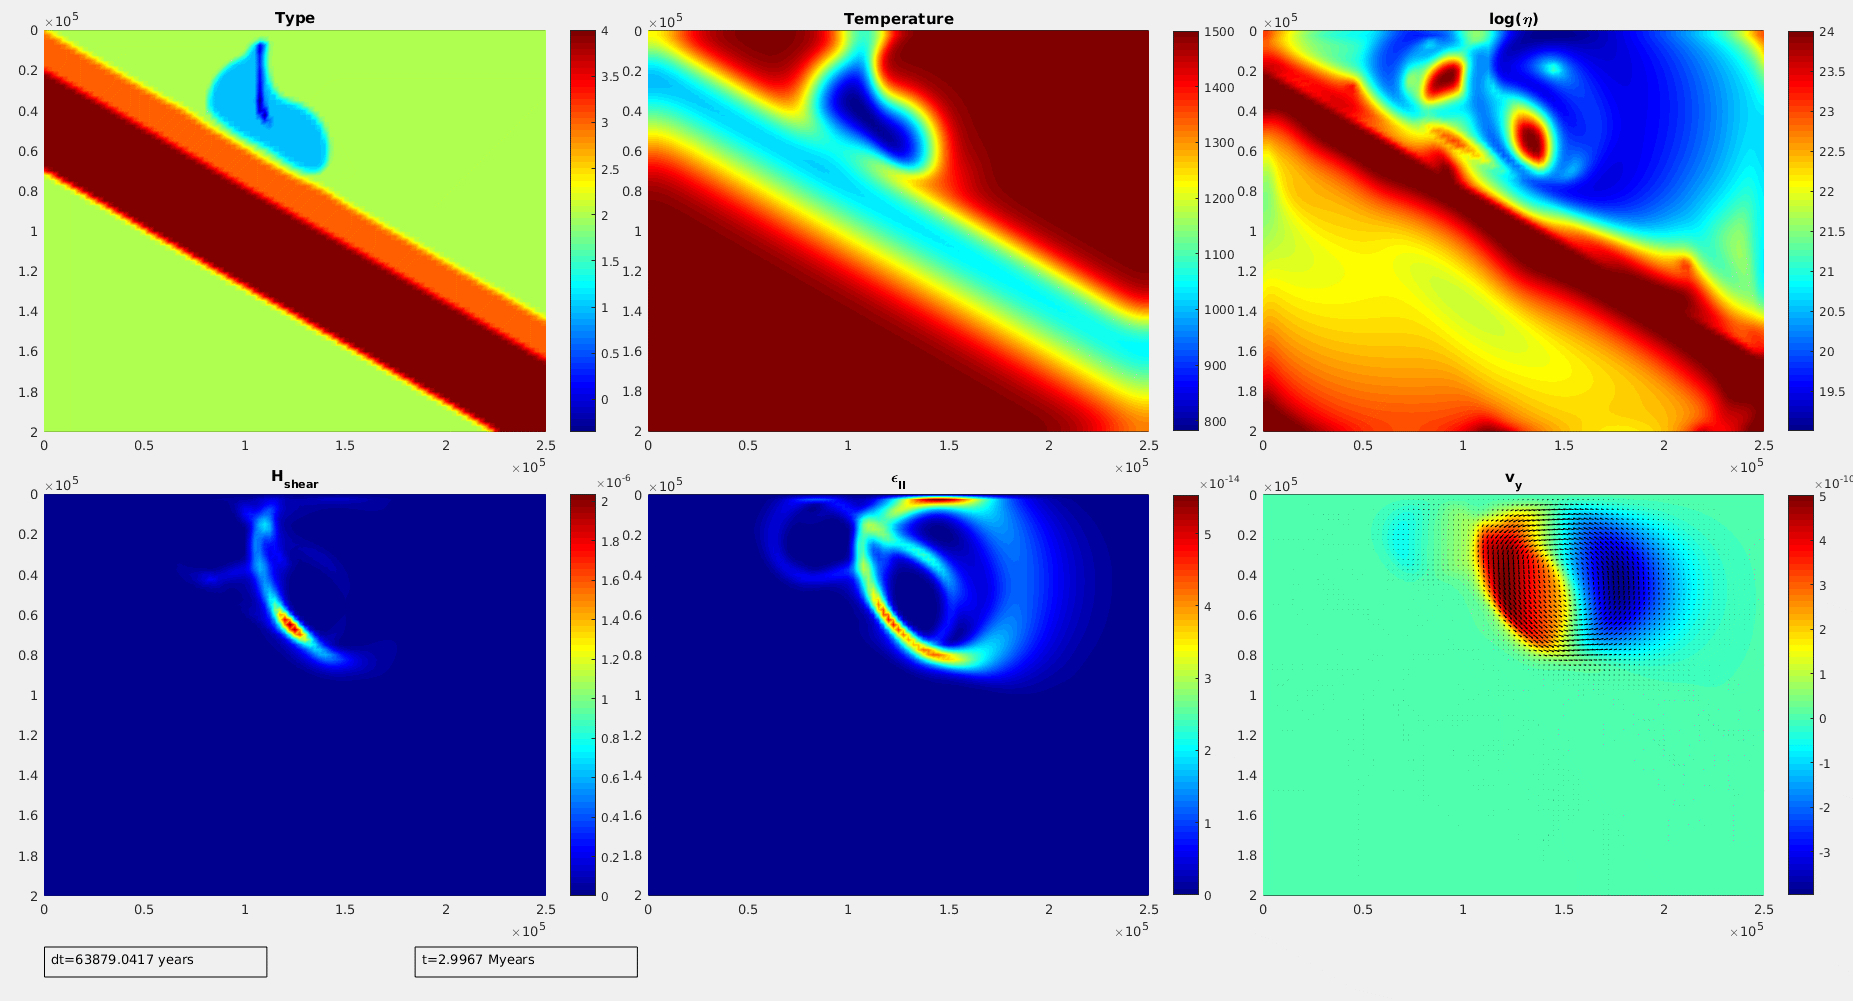
\includegraphics[width=1.0\textwidth]{./Snapshots/ref/Subductionzonewithblobpos1slab30s1e7r25.jpg}
\end{minipage}
\caption{3 million years later in scenario 30 degrees with radius 25km}
\label{fig:3m3025km}
\end{figure}
\begin{figure}
\begin{minipage}[t]{1.0\textwidth}
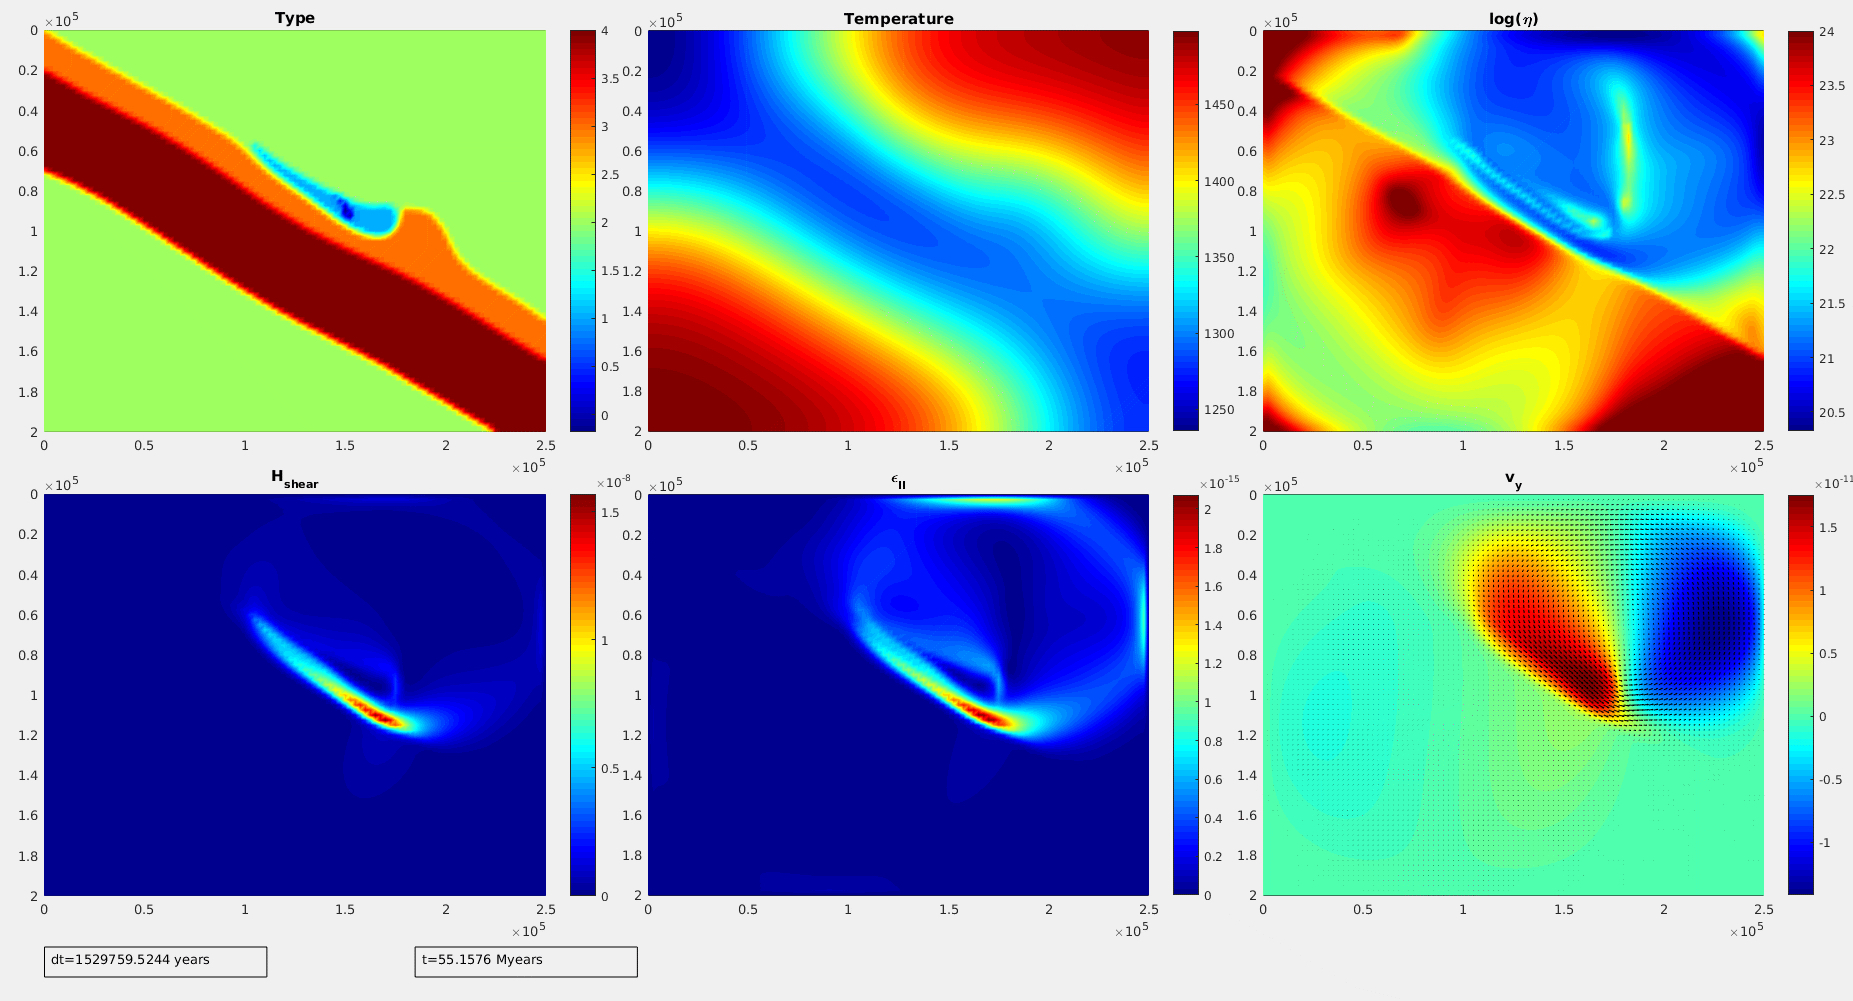
\includegraphics[width=1.0\textwidth]{./Snapshots/ref/Subductionzonewithblobpos1slab30s1e7r15.jpg}
\end{minipage}
\caption{55 million years later in scenario 30 degrees with radius 15km}
\label{fig:55m3015km}
\end{figure}

%\newpage
\subsection{Rotation of the plume}
Here the rotation profile of the plume is more closely examined. The rotation profile is constructed with the help of the topmost material particle in the plume. This particle was tracked throughout the simulation and its calculated $v_x$ velocity together with the timestep $d t$ was used to approximate the displacement along the plume and thus the angle of rotation. This works fine for the first 20-30 timesteps where there is no deformation and as long as the plume has not rotated more than 90 degrees but still it is more precise than to solely measured with naked eyes. In figure \ref{fig:rotationinitial} the rotation of our reference initial state is depicted. The time to end the profile was chosen such that it corresponds close to the point in time where the plume "stops" because of "collision" and starts deformation and further possible rotation. Important to note is that the profile is difficult to compare across plate angles since different angle implies different position for the plume and therefore different distance between plume and plate and therefore different times until collision. However there is a clear trend that when the available space on the left side of the plume shrinks the shifting of material from left to right slows considerably such that there is much less rotation.

\begin{figure}[!ht]
	\begin{minipage}[t]{1.0\textwidth}
		\begin{minipage}[t]{0.5\textwidth}		
		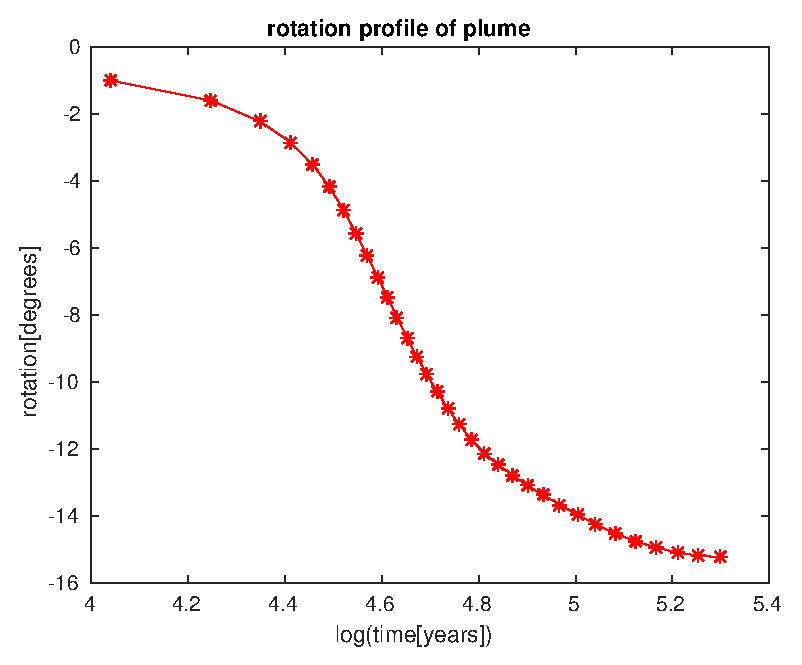
\includegraphics[width=1.0\textwidth]{./Snapshots/ref/Subductionzonewithblobposrefslab20s2e7s2e7r20rotation.eps}
		\end{minipage}
		\begin{minipage}[t]{0.5\textwidth}
		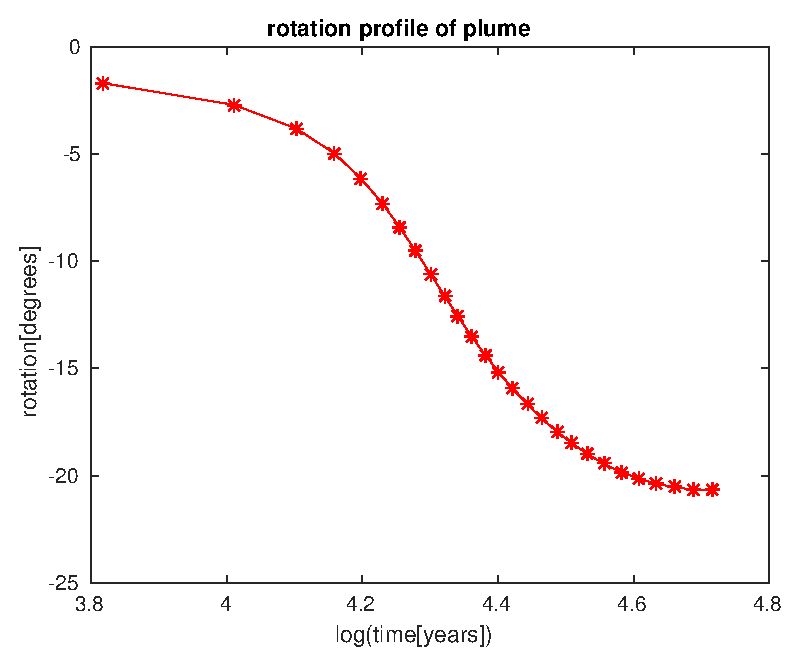
\includegraphics[width=1.0\textwidth]{./Snapshots/ref/Subductionzonewithblobposrefslab30s2e7s2e7r20rotation.eps}
		\end{minipage}
	\end{minipage}
	\begin{minipage}[t]{1.0\textwidth}	
		\begin{minipage}[t]{0.5\textwidth}
		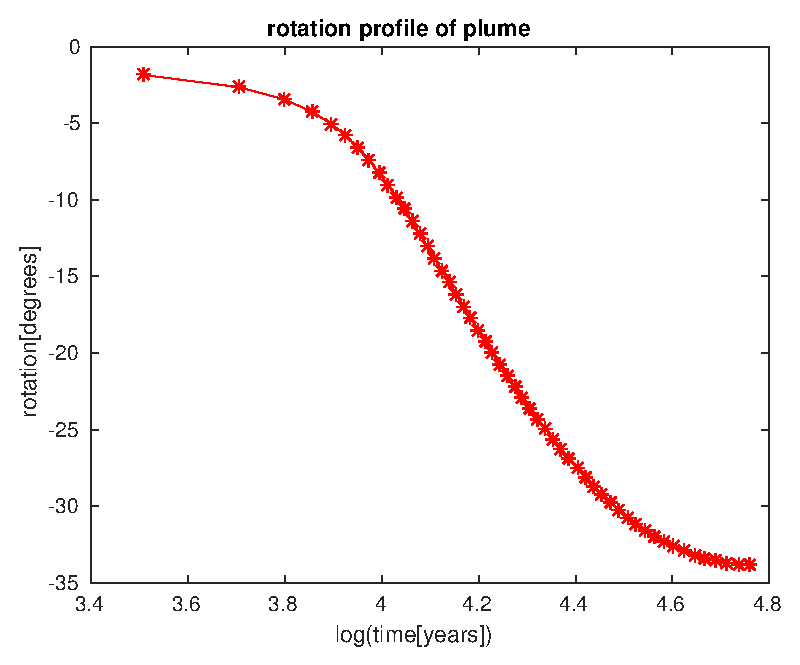
\includegraphics[width=1.0\textwidth]{./Snapshots/ref/Subductionzonewithblobposrefslab45s2e7s2e7r20rotation.eps}
		\end{minipage}
		\begin{minipage}[t]{0.5\textwidth}
		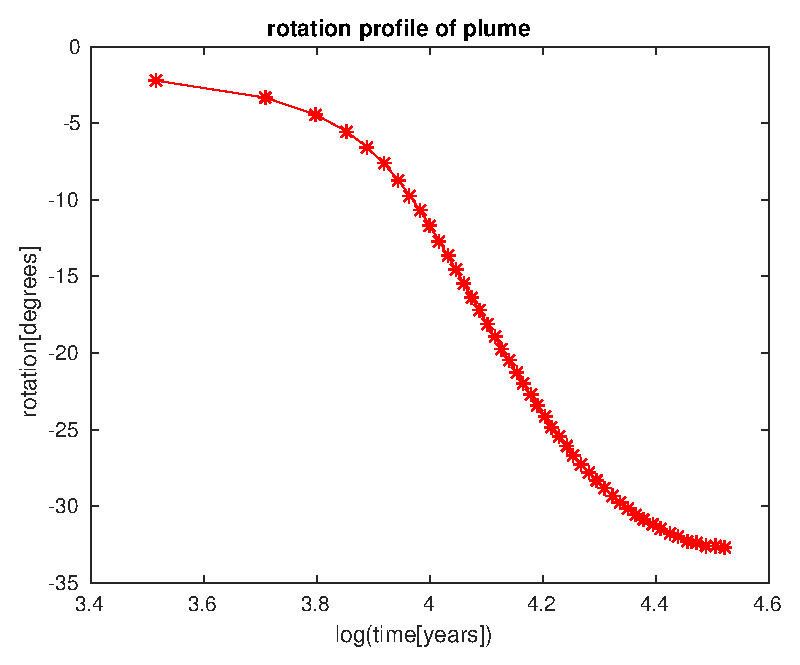
\includegraphics[width=1.0\textwidth]{./Snapshots/ref/Subductionzonewithblobposrefslab60s2e7s2e7r20rotation.eps}
		\end{minipage}
	\end{minipage}
	\caption{rotation of the plume with 20(top left), 30(top right), 45(bottom left) and 60(bottom right) degree angle of the plate}
	\label{fig:rotationinitial}
\end{figure}


\subsection{Velocity of the plume}
In this section the velocity profile is investigated. To produce such an profile the same material particle as in the previous section of rotation was utilized to measure in this case the $v_y$ velocity along with time. One can see from the profile in figure \ref{fig:velocityinitial} the interesting phases which are first acceleration in the beginning with a peak velocity in half time point until collision and thereafter the braking phase until the collision. The different peak velocities also coincide with the distance between plume and plane as expected. Higher distance implies more time for acceleration which further implies higher velocity peak. Interesting differences could be seen in variating the radius or the strengths which will be done later on.

\begin{figure}[ht!]
	\begin{minipage}[t]{1.0\textwidth}
		\begin{minipage}[t]{0.5\textwidth}
		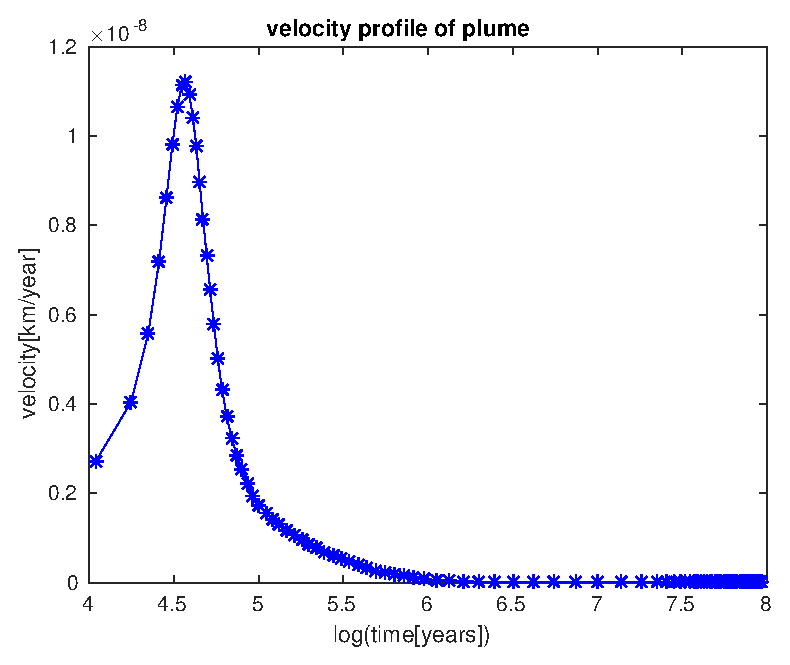
\includegraphics[width=1.0\textwidth]{./Snapshots/ref/Subductionzonewithblobposrefslab20s2e7s2e7r20velocity.eps}
		\end{minipage}
		\begin{minipage}[t]{0.5\textwidth}
		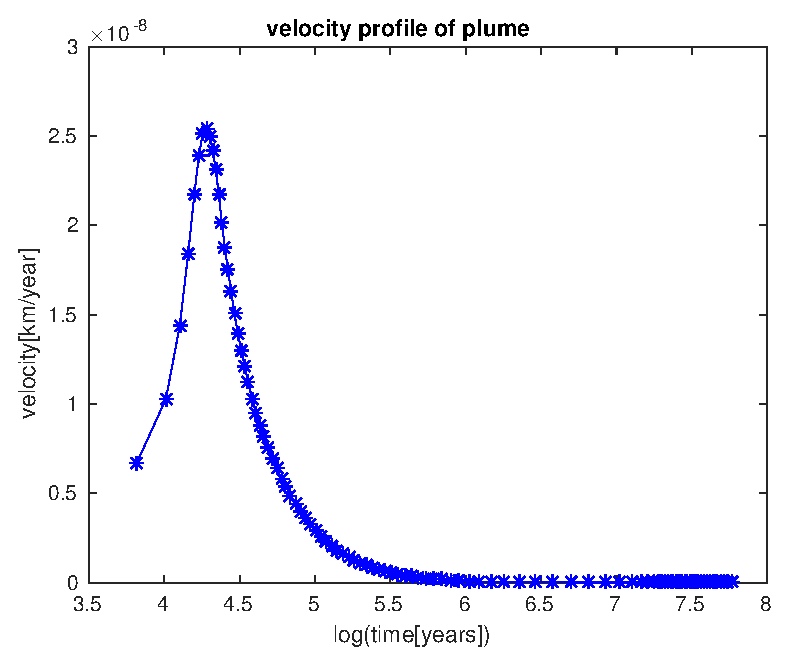
\includegraphics[width=1.0\textwidth]{./Snapshots/ref/Subductionzonewithblobposrefslab30s2e7s2e7r20velocity.eps}
		\end{minipage}
	\end{minipage}
	\begin{minipage}[t]{1.0\textwidth}	
		\begin{minipage}[t]{0.5\textwidth}
		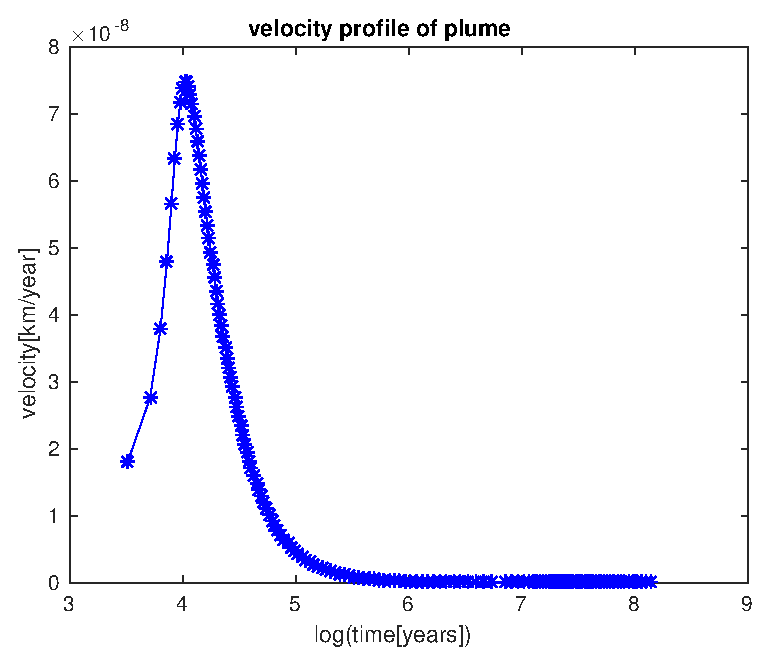
\includegraphics[width=1.0\textwidth]{./Snapshots/ref/Subductionzonewithblobposrefslab45s2e7s2e7r20velocity.eps}
		\end{minipage}
		\begin{minipage}[t]{0.5\textwidth}
		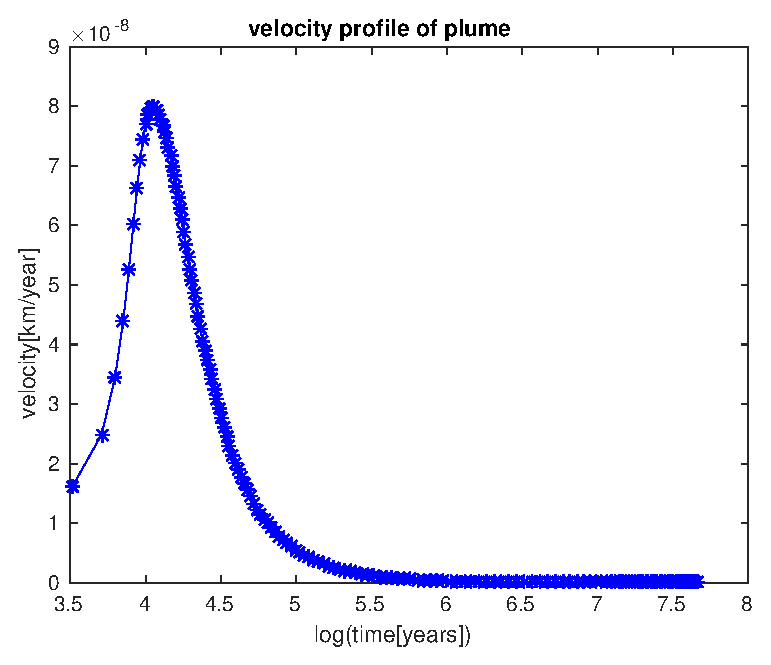
\includegraphics[width=1.0\textwidth]{./Snapshots/ref/Subductionzonewithblobposrefslab60s2e7s2e7r20velocity.eps}
		\end{minipage}
	\end{minipage}
	\caption{velocity of the plume with 20(top left), 30(top right), 45(bottom left) and 60(bottom right) degree angle of the plate}
	\label{fig:velocityinitial}
\end{figure}

\subsection{Rotation and velocity analysis}
As already mentioned in this section the interaction between the parameters and the resulting rotation and velocity profiles is explored. These studies were done at the example of reference position with variation in radius and variation in sigma for the plate. The results are shown in figures \ref{fig:mixsigma45} and \ref{fig:mixsigma60}. The trend hereby is conclusive in both cases. The influence from the variation in the strength $\sigma$ negligible for the profiles. Whereas the influence of the radius is significant for the shape of the profiles. The higher the radius the steeper is the rotation profile and the higher is the peak velocity. Only the cases of 45 degrees and 60 degrees angle was considered since in both other cases there is distortion of the plate due to lack of space and therefore the profiles are not usable.

\begin{figure}[ht!]
	\begin{minipage}[t]{1.0\textwidth}
		\begin{minipage}[t]{0.5\textwidth}
		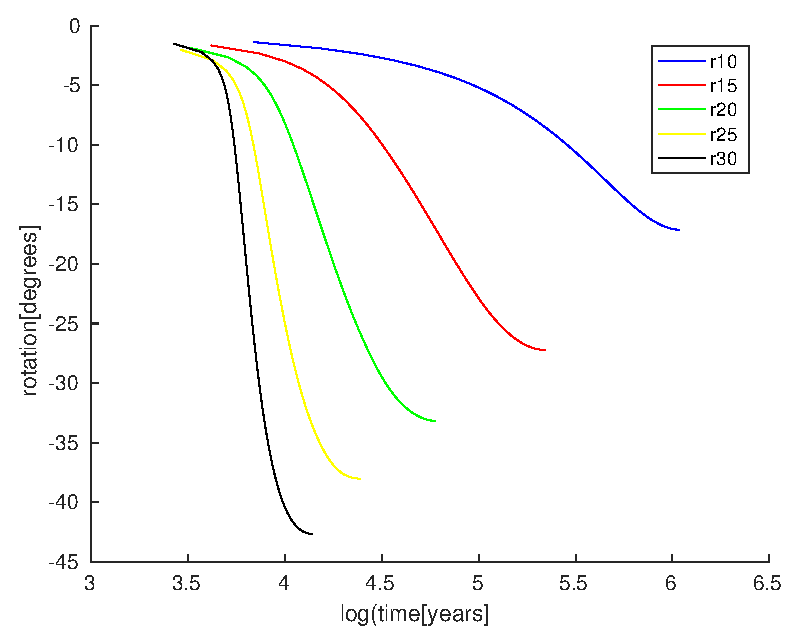
\includegraphics[width=1.0\textwidth]{./Snapshots/slab45s1e8mixedr_rot.eps}
		\end{minipage}
		\begin{minipage}[t]{0.5\textwidth}
		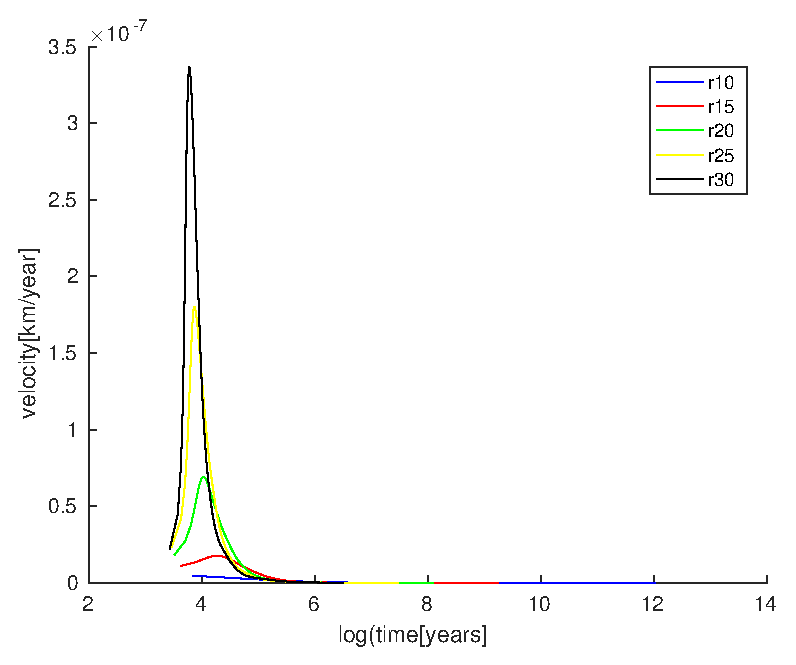
\includegraphics[width=1.0\textwidth]{./Snapshots/slab45s1e8mixedr_vel.eps}
		\end{minipage}
	\end{minipage}
	\begin{minipage}[t]{1.0\textwidth}	
		\begin{minipage}[t]{0.5\textwidth}
		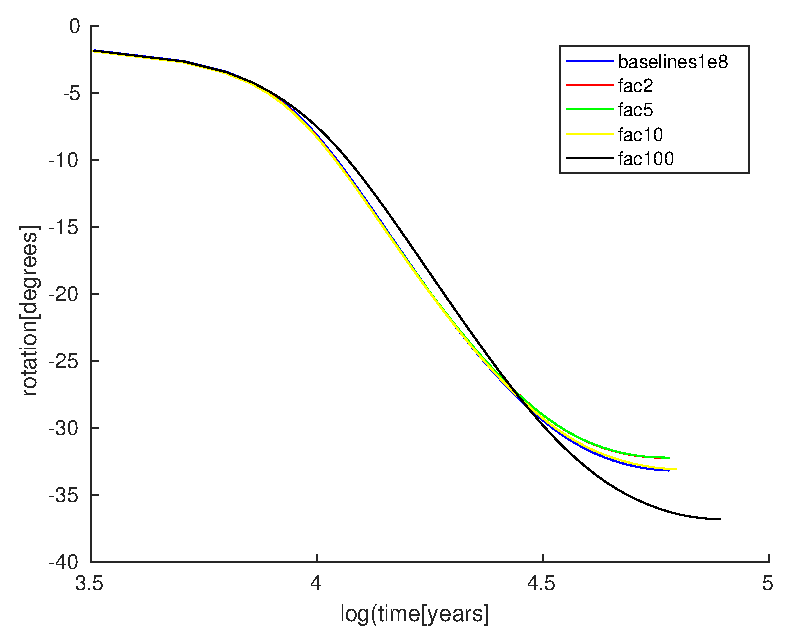
\includegraphics[width=1.0\textwidth]{./Snapshots/slab45s1e8mixedsigma_rot.eps}
		\end{minipage}
		\begin{minipage}[t]{0.5\textwidth}
		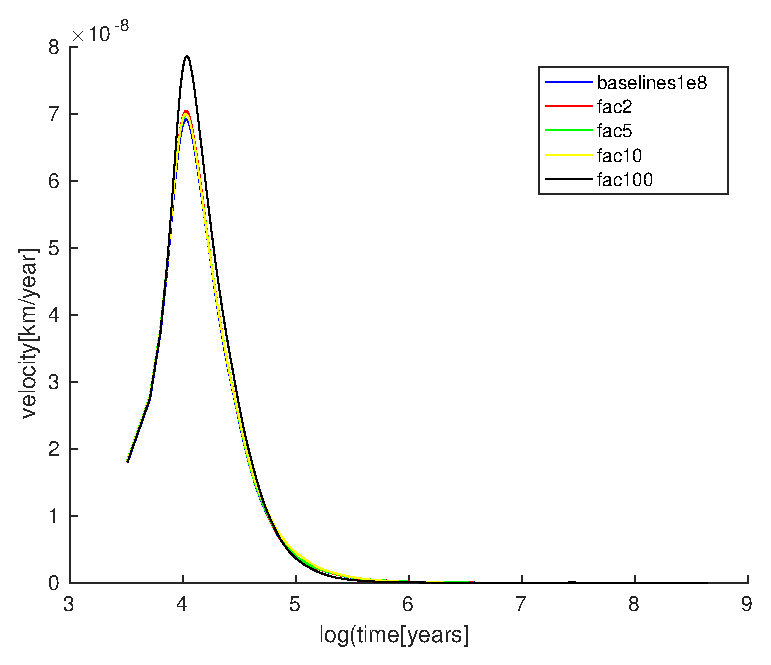
\includegraphics[width=1.0\textwidth]{./Snapshots/slab45s1e8mixedsigma_vel.eps}
		\end{minipage}
	\end{minipage}
	\caption{Mixed sigma and radii in case of 45 degrees angle}
	\label{fig:mixsigma45}
\end{figure}

\begin{figure}[ht!]
	\begin{minipage}[t]{1.0\textwidth}
		\begin{minipage}[t]{0.5\textwidth}
		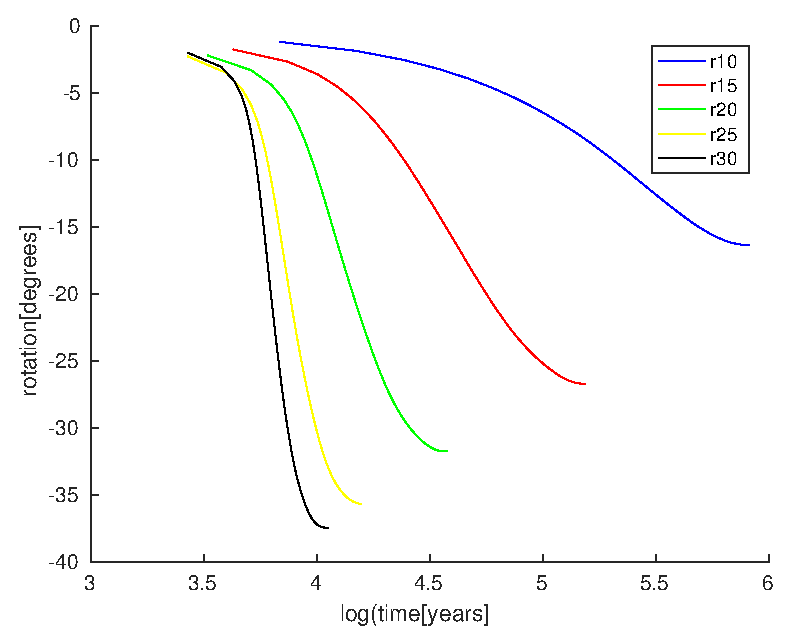
\includegraphics[width=1.0\textwidth]{./Snapshots/slab60s1e8mixedr_rot.eps}
		\end{minipage}
		\begin{minipage}[t]{0.5\textwidth}
		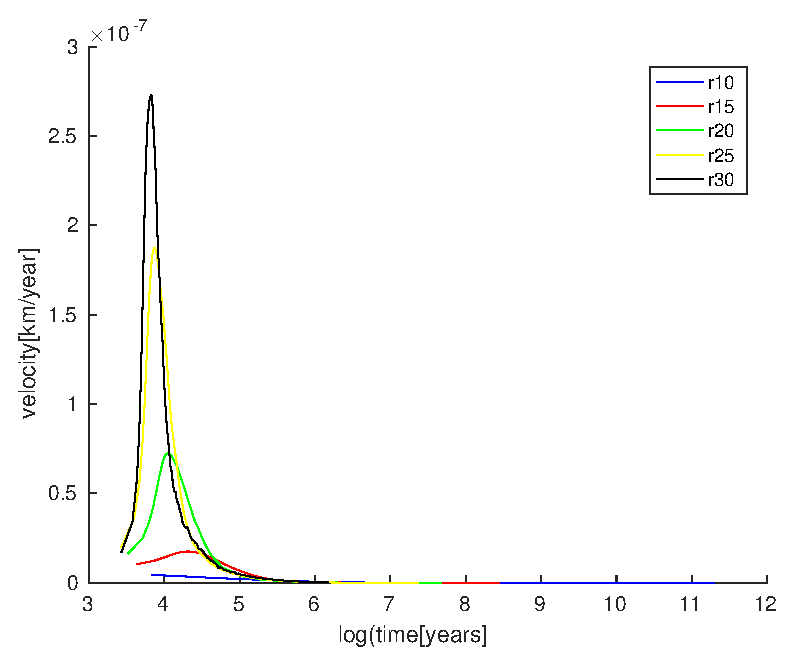
\includegraphics[width=1.0\textwidth]{./Snapshots/slab60s1e8mixedr_vel.eps}
		\end{minipage}
	\end{minipage}
	\begin{minipage}[t]{1.0\textwidth}	
		\begin{minipage}[t]{0.5\textwidth}
		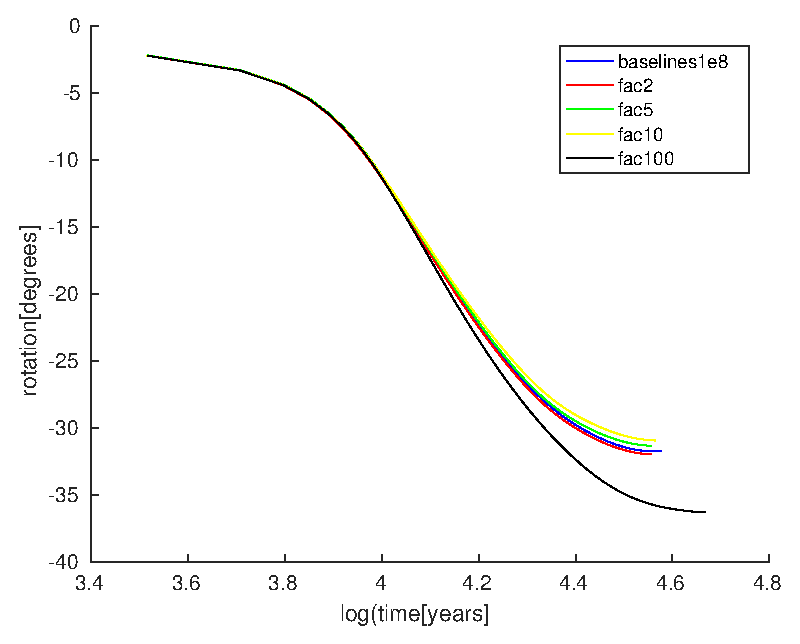
\includegraphics[width=1.0\textwidth]{./Snapshots/slab60s1e8mixedsigma_rot.eps}
		\end{minipage}
		\begin{minipage}[t]{0.5\textwidth}
		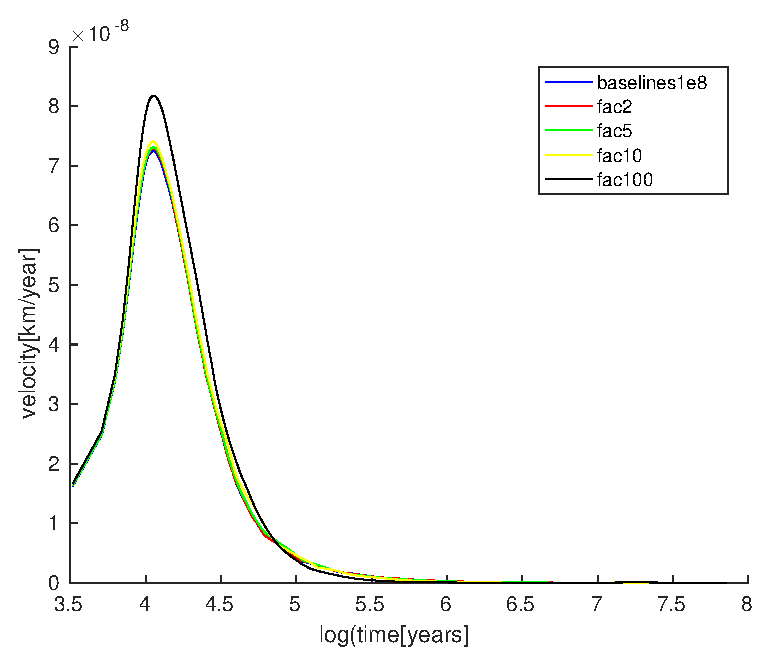
\includegraphics[width=1.0\textwidth]{./Snapshots/slab60s1e8mixedsigma_vel.eps}
		\end{minipage}
	\end{minipage}
	\caption{Mixed sigma and radii in case of 60 degrees angle}
	\label{fig:mixsigma60}
\end{figure}

There was also an additional interesting case when the position of the plume was shifted to the right. In this case the space on the right side was not dominant in producing the velocity field and therefore the plume started rotating in the other direction. After the plume sunk enough to reduce the space on the left side the plume rotated back to the initial position and then further shown in figure \ref{fig:introtprof}.

\begin{figure}[ht!]
\begin{minipage}[t]{1.0\textwidth}
		\begin{minipage}[t]{0.5\textwidth}
		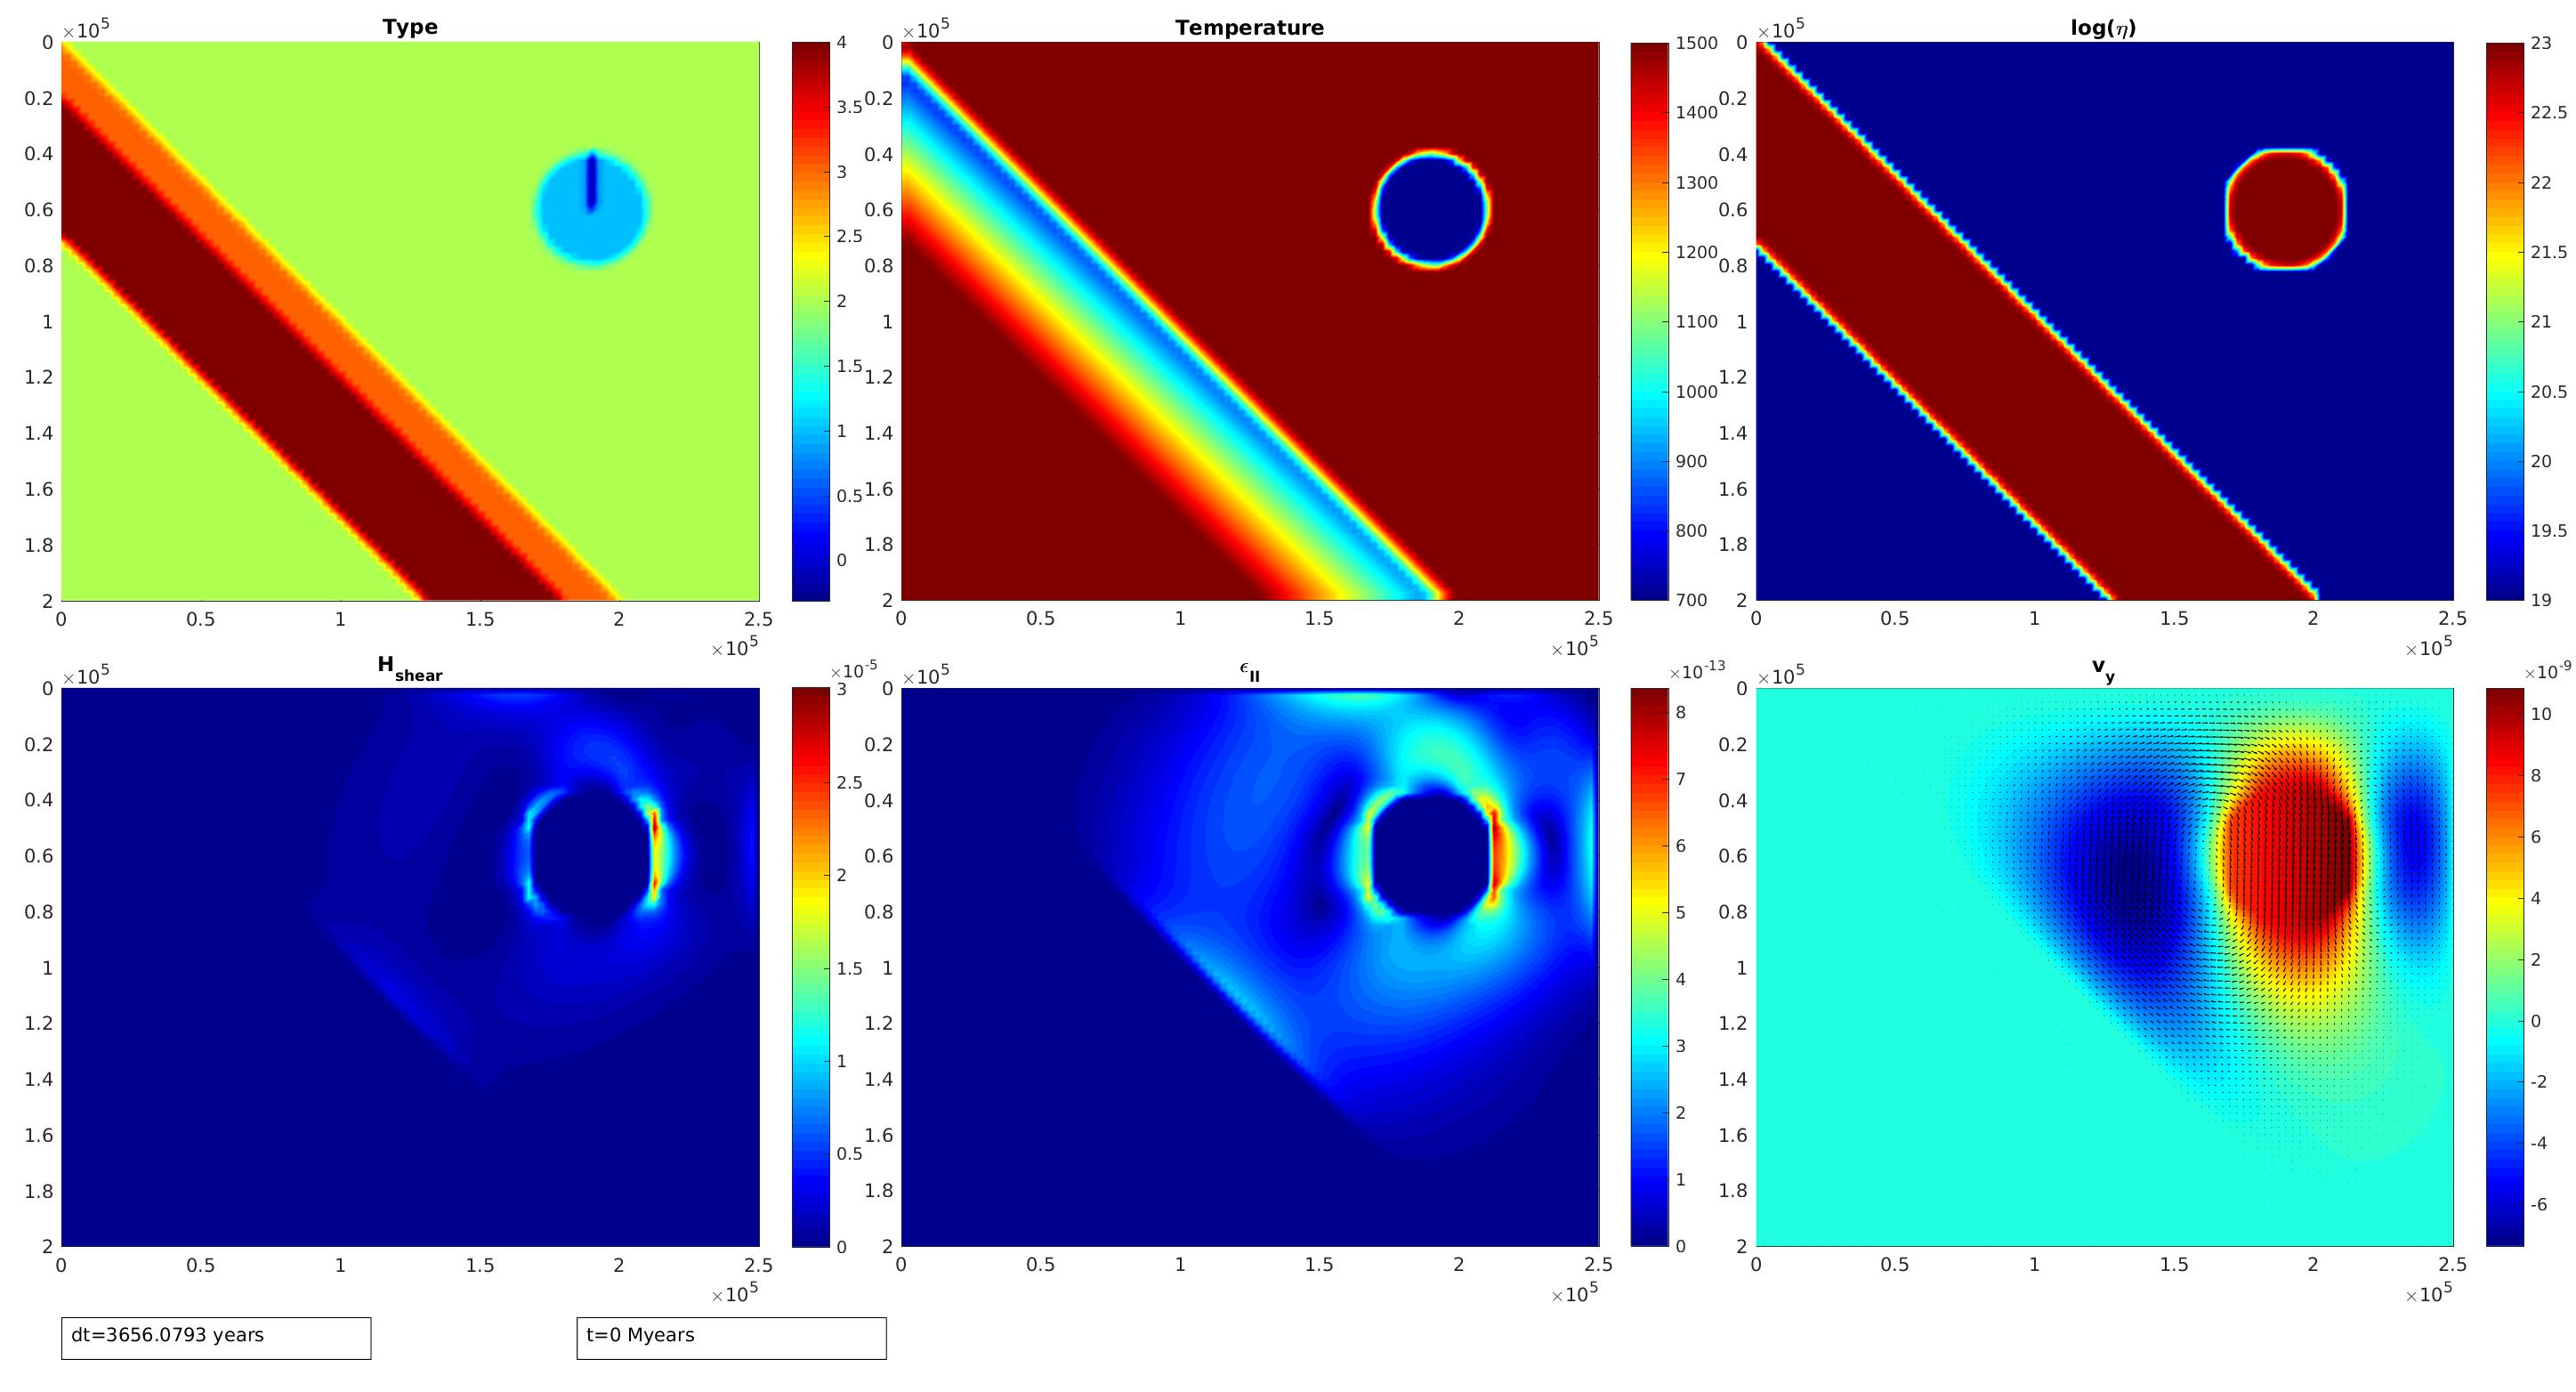
\includegraphics[width=1.0\textwidth]{./Snapshots/pos2/Subductionzonewithblob1pos2slab45s2e7s2e7r20.jpg}
		\end{minipage}
		\begin{minipage}[t]{0.5\textwidth}
		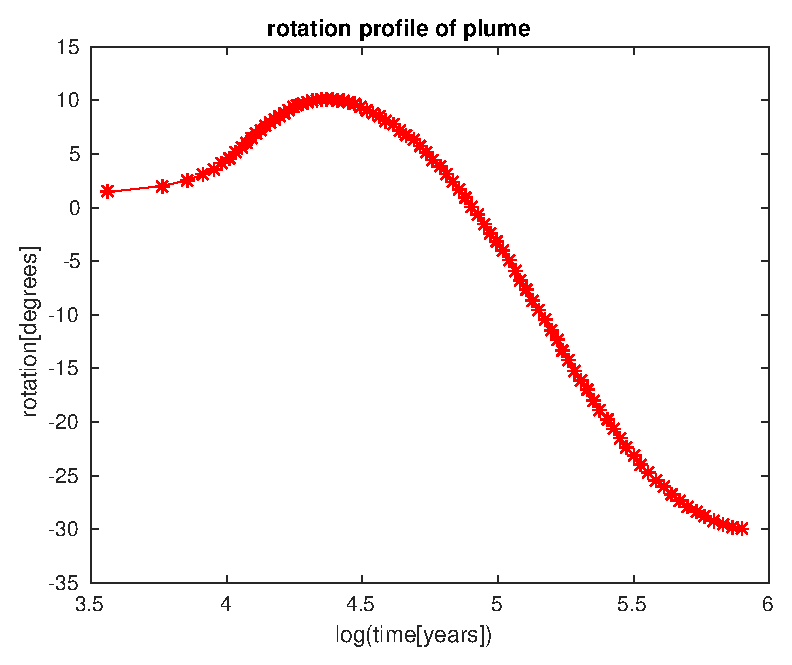
\includegraphics[width=1.0\textwidth]{./Snapshots/pos2/Subductionzonewithblobpos2slab45s2e7s2e7r20rotation.eps}
		\end{minipage}
	\end{minipage}
	\caption{45 degrees slab with shifted position to the right}
	\label{fig:introtprof}
\end{figure}

\subsection{Bulldozer effect}
First only the 45 degrees angle was considered for producing a bulldozer effect. Thereby the strength was first varied where the results of the distortion is presented in figure \ref{fig:bulldozer45}. As one can see they all produced all similar spiked distortions with different intensity. The intensity hereby was dependent on the difference in strength of the plume and plate. The factors of difference were 100(top left $10^8/10^6$), 50(top right $5\cdot 10^7/10^6$), 5(bottom left $5\cdot 10^7/10^7$) and 2(bottom right $2\cdot 10^7/10^7$). This is not similar to the desired shape like in \ref{fig:55m3015km}. Therefore next only 30 degrees scenario was closer examined.

\begin{figure}[!ht]
	\begin{minipage}[t]{1.0\textwidth}
		\begin{minipage}[t]{0.5\textwidth}
			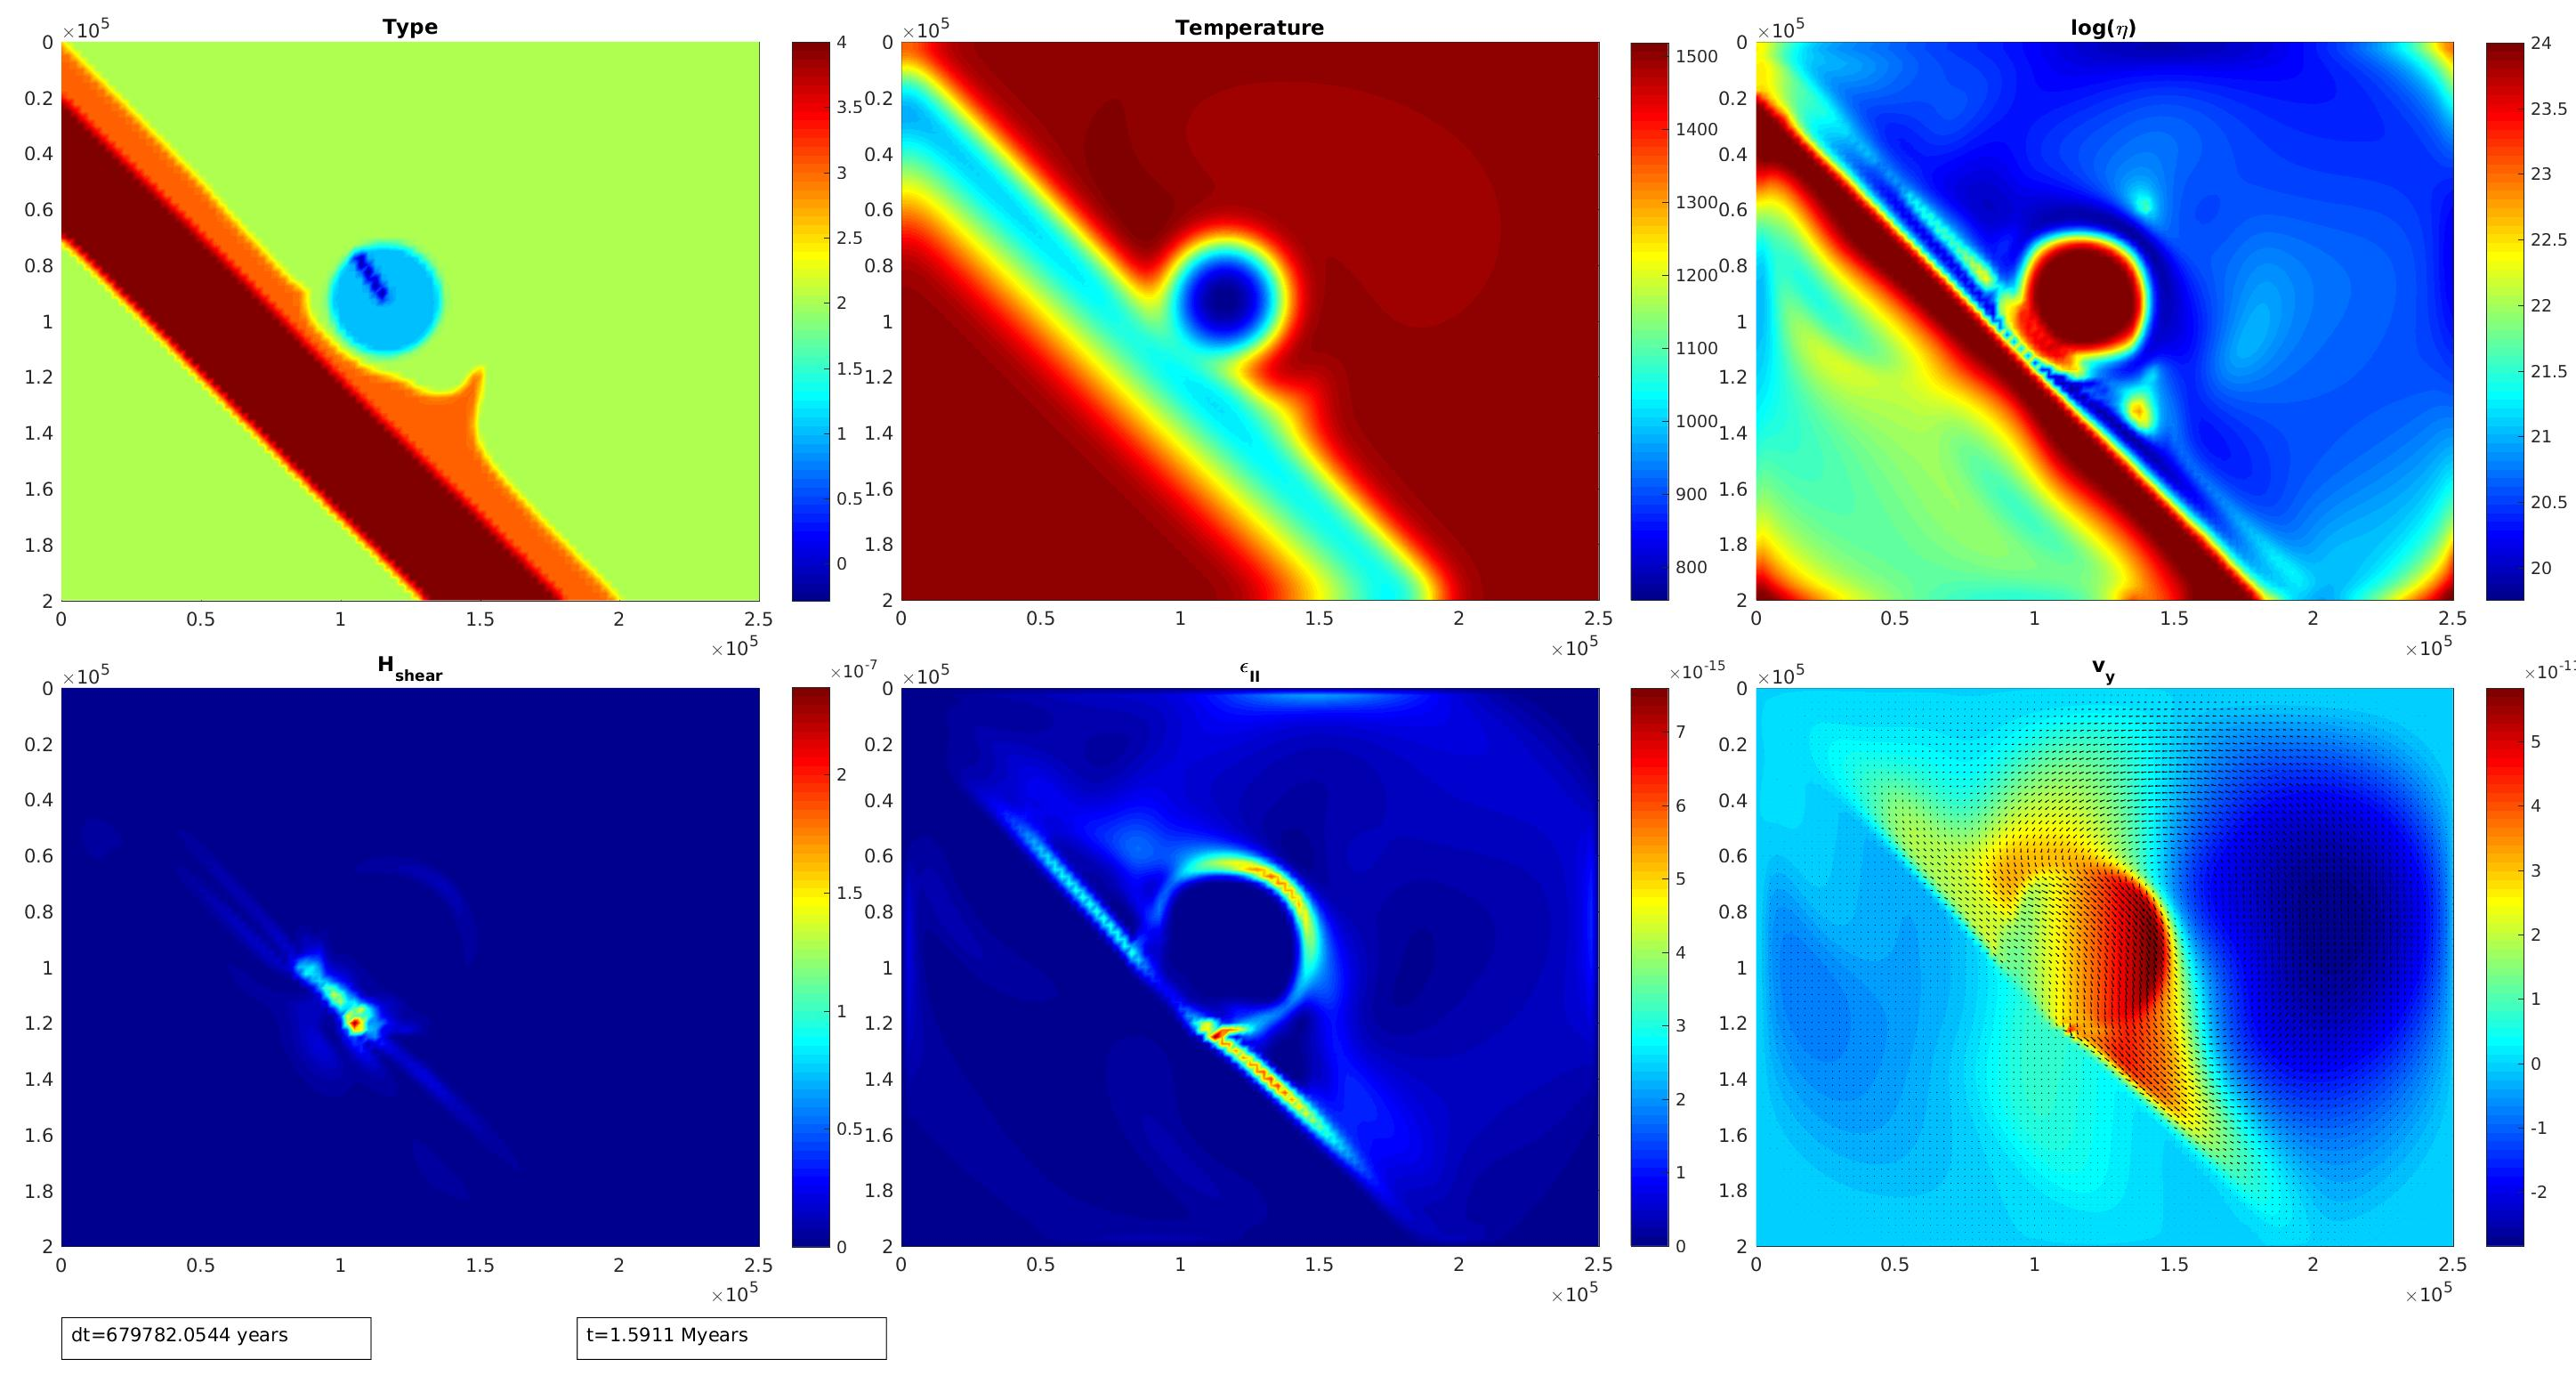
\includegraphics[width=1.0\textwidth]{./Snapshots/bulldozer/posleft45/Subductionzonewithblob67posleftslab45s1e8s1e6r20.jpg}
		\end{minipage}
		\begin{minipage}[t]{0.5\textwidth}
			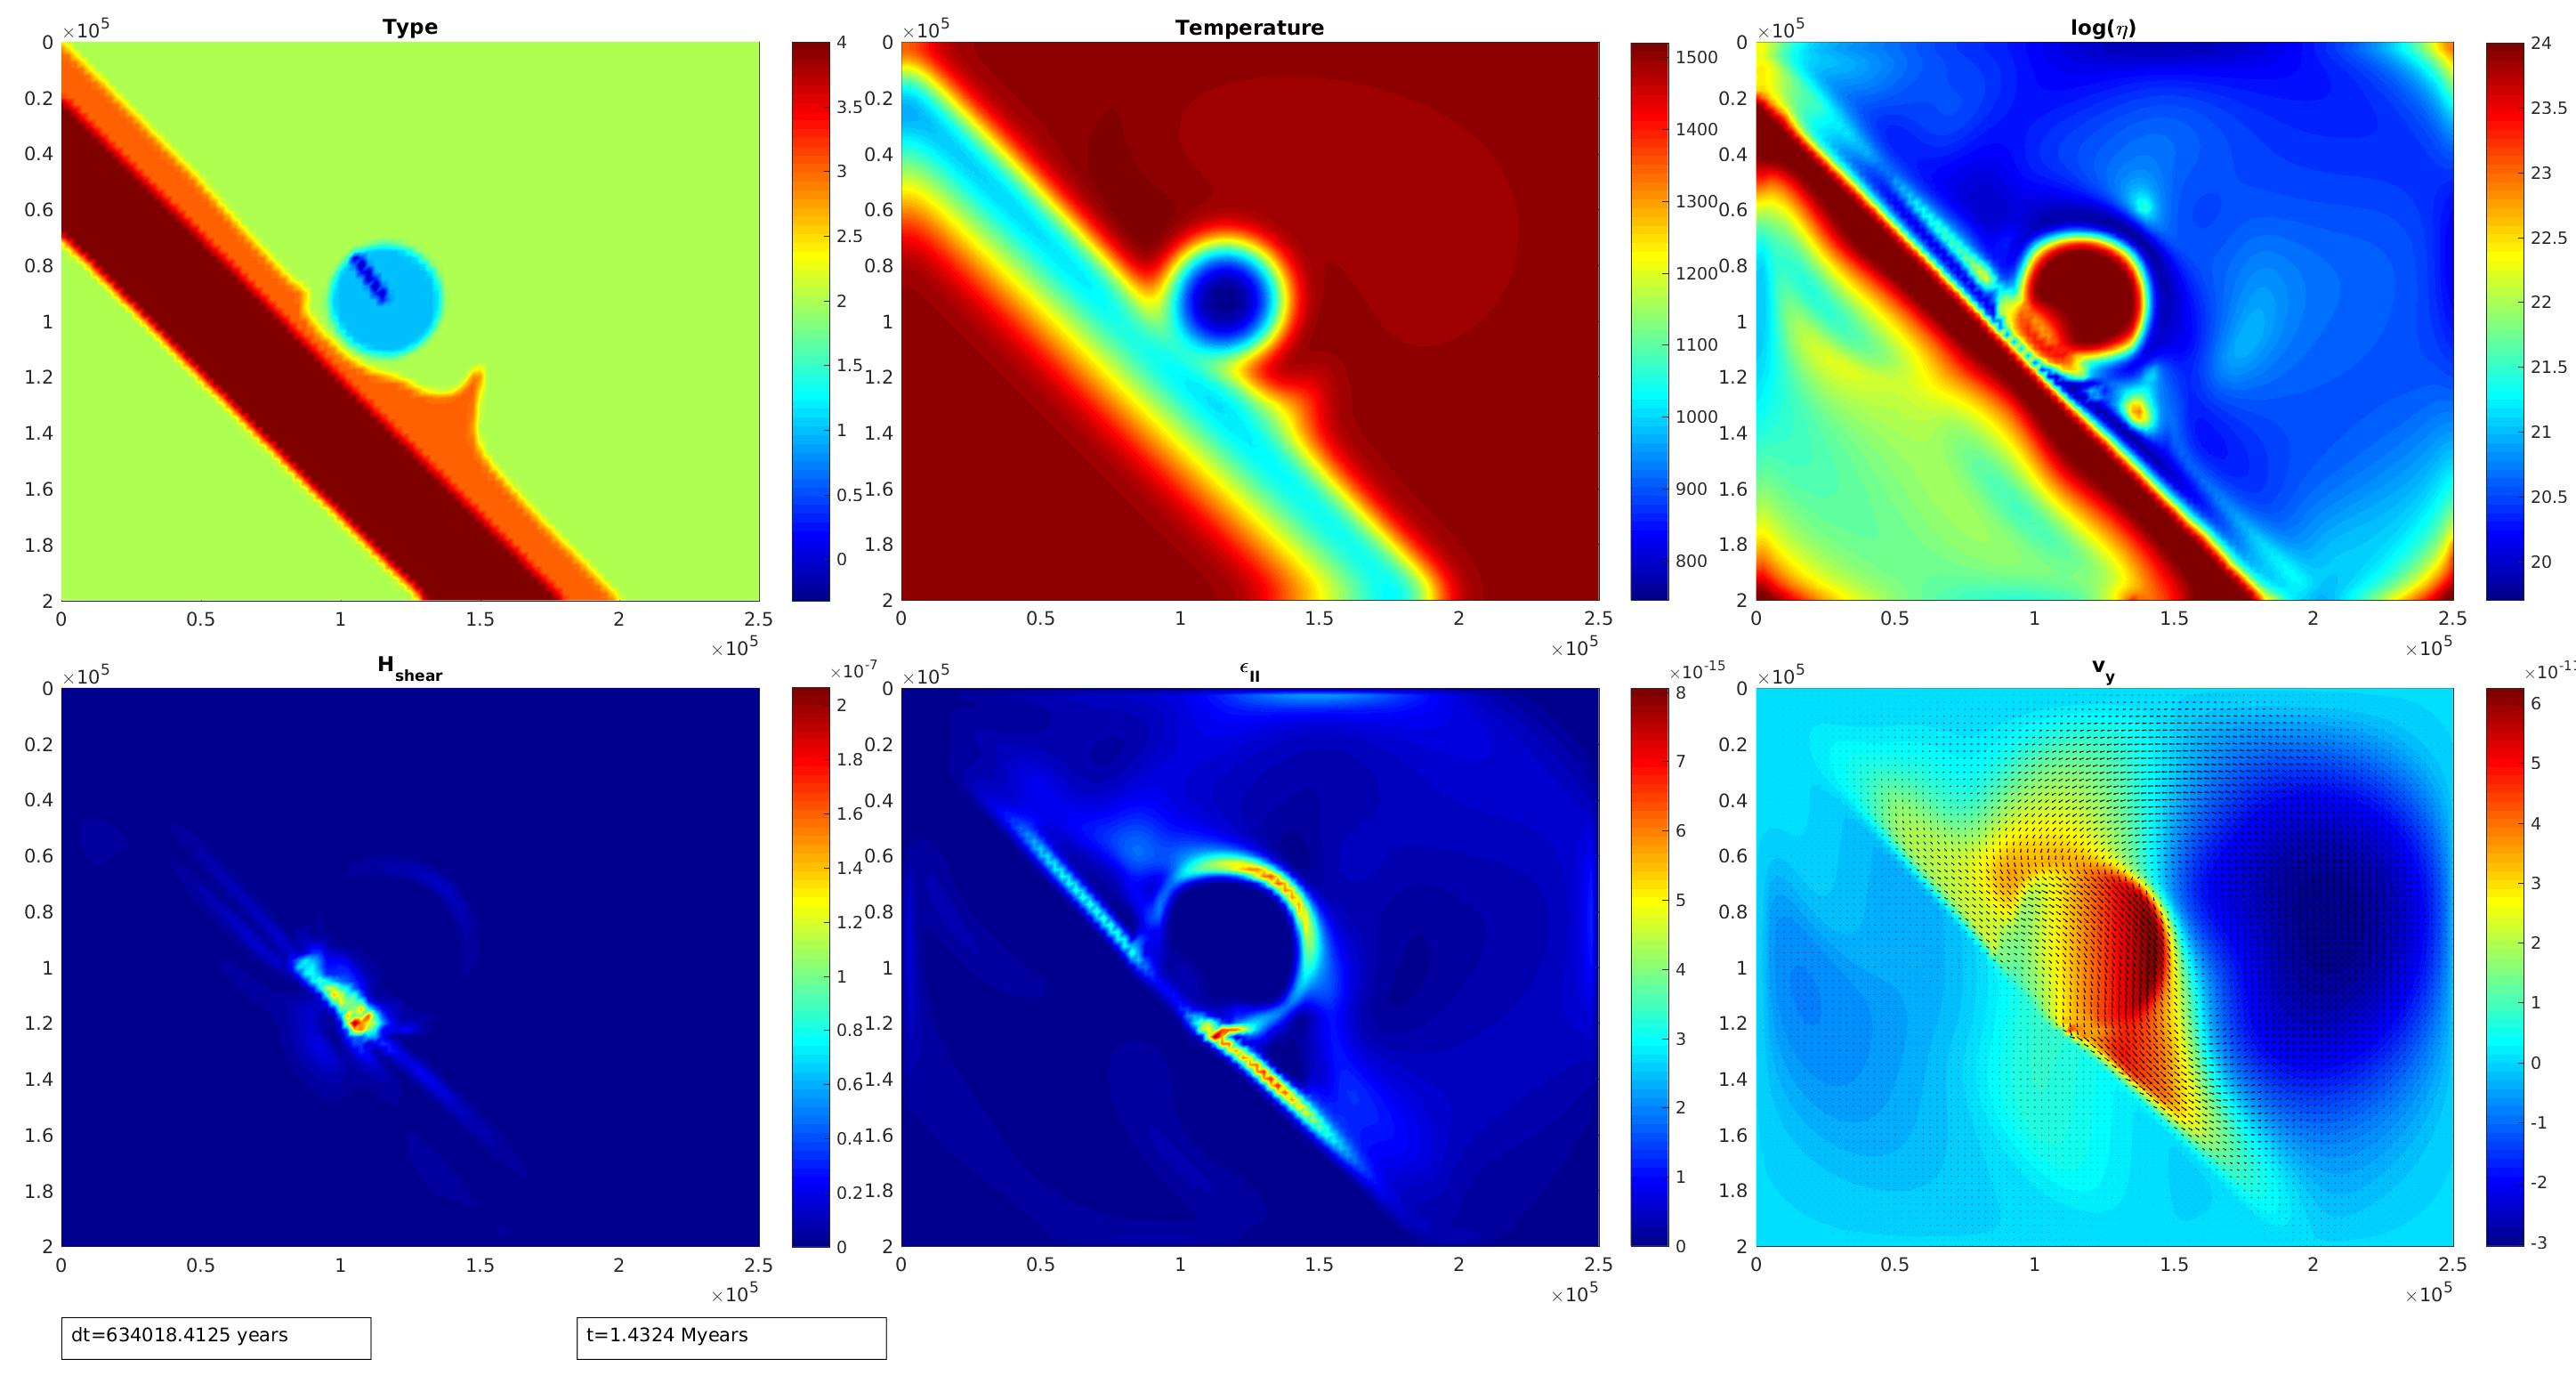
\includegraphics[width=1.0\textwidth]{./Snapshots/bulldozer/posleft45/Subductionzonewithblob67posleftslab45s5e7s1e6r20.jpg}
		\end{minipage}
	\end{minipage}
	\begin{minipage}[c]{1.0\textwidth}
		\begin{minipage}[t]{0.5\textwidth}
			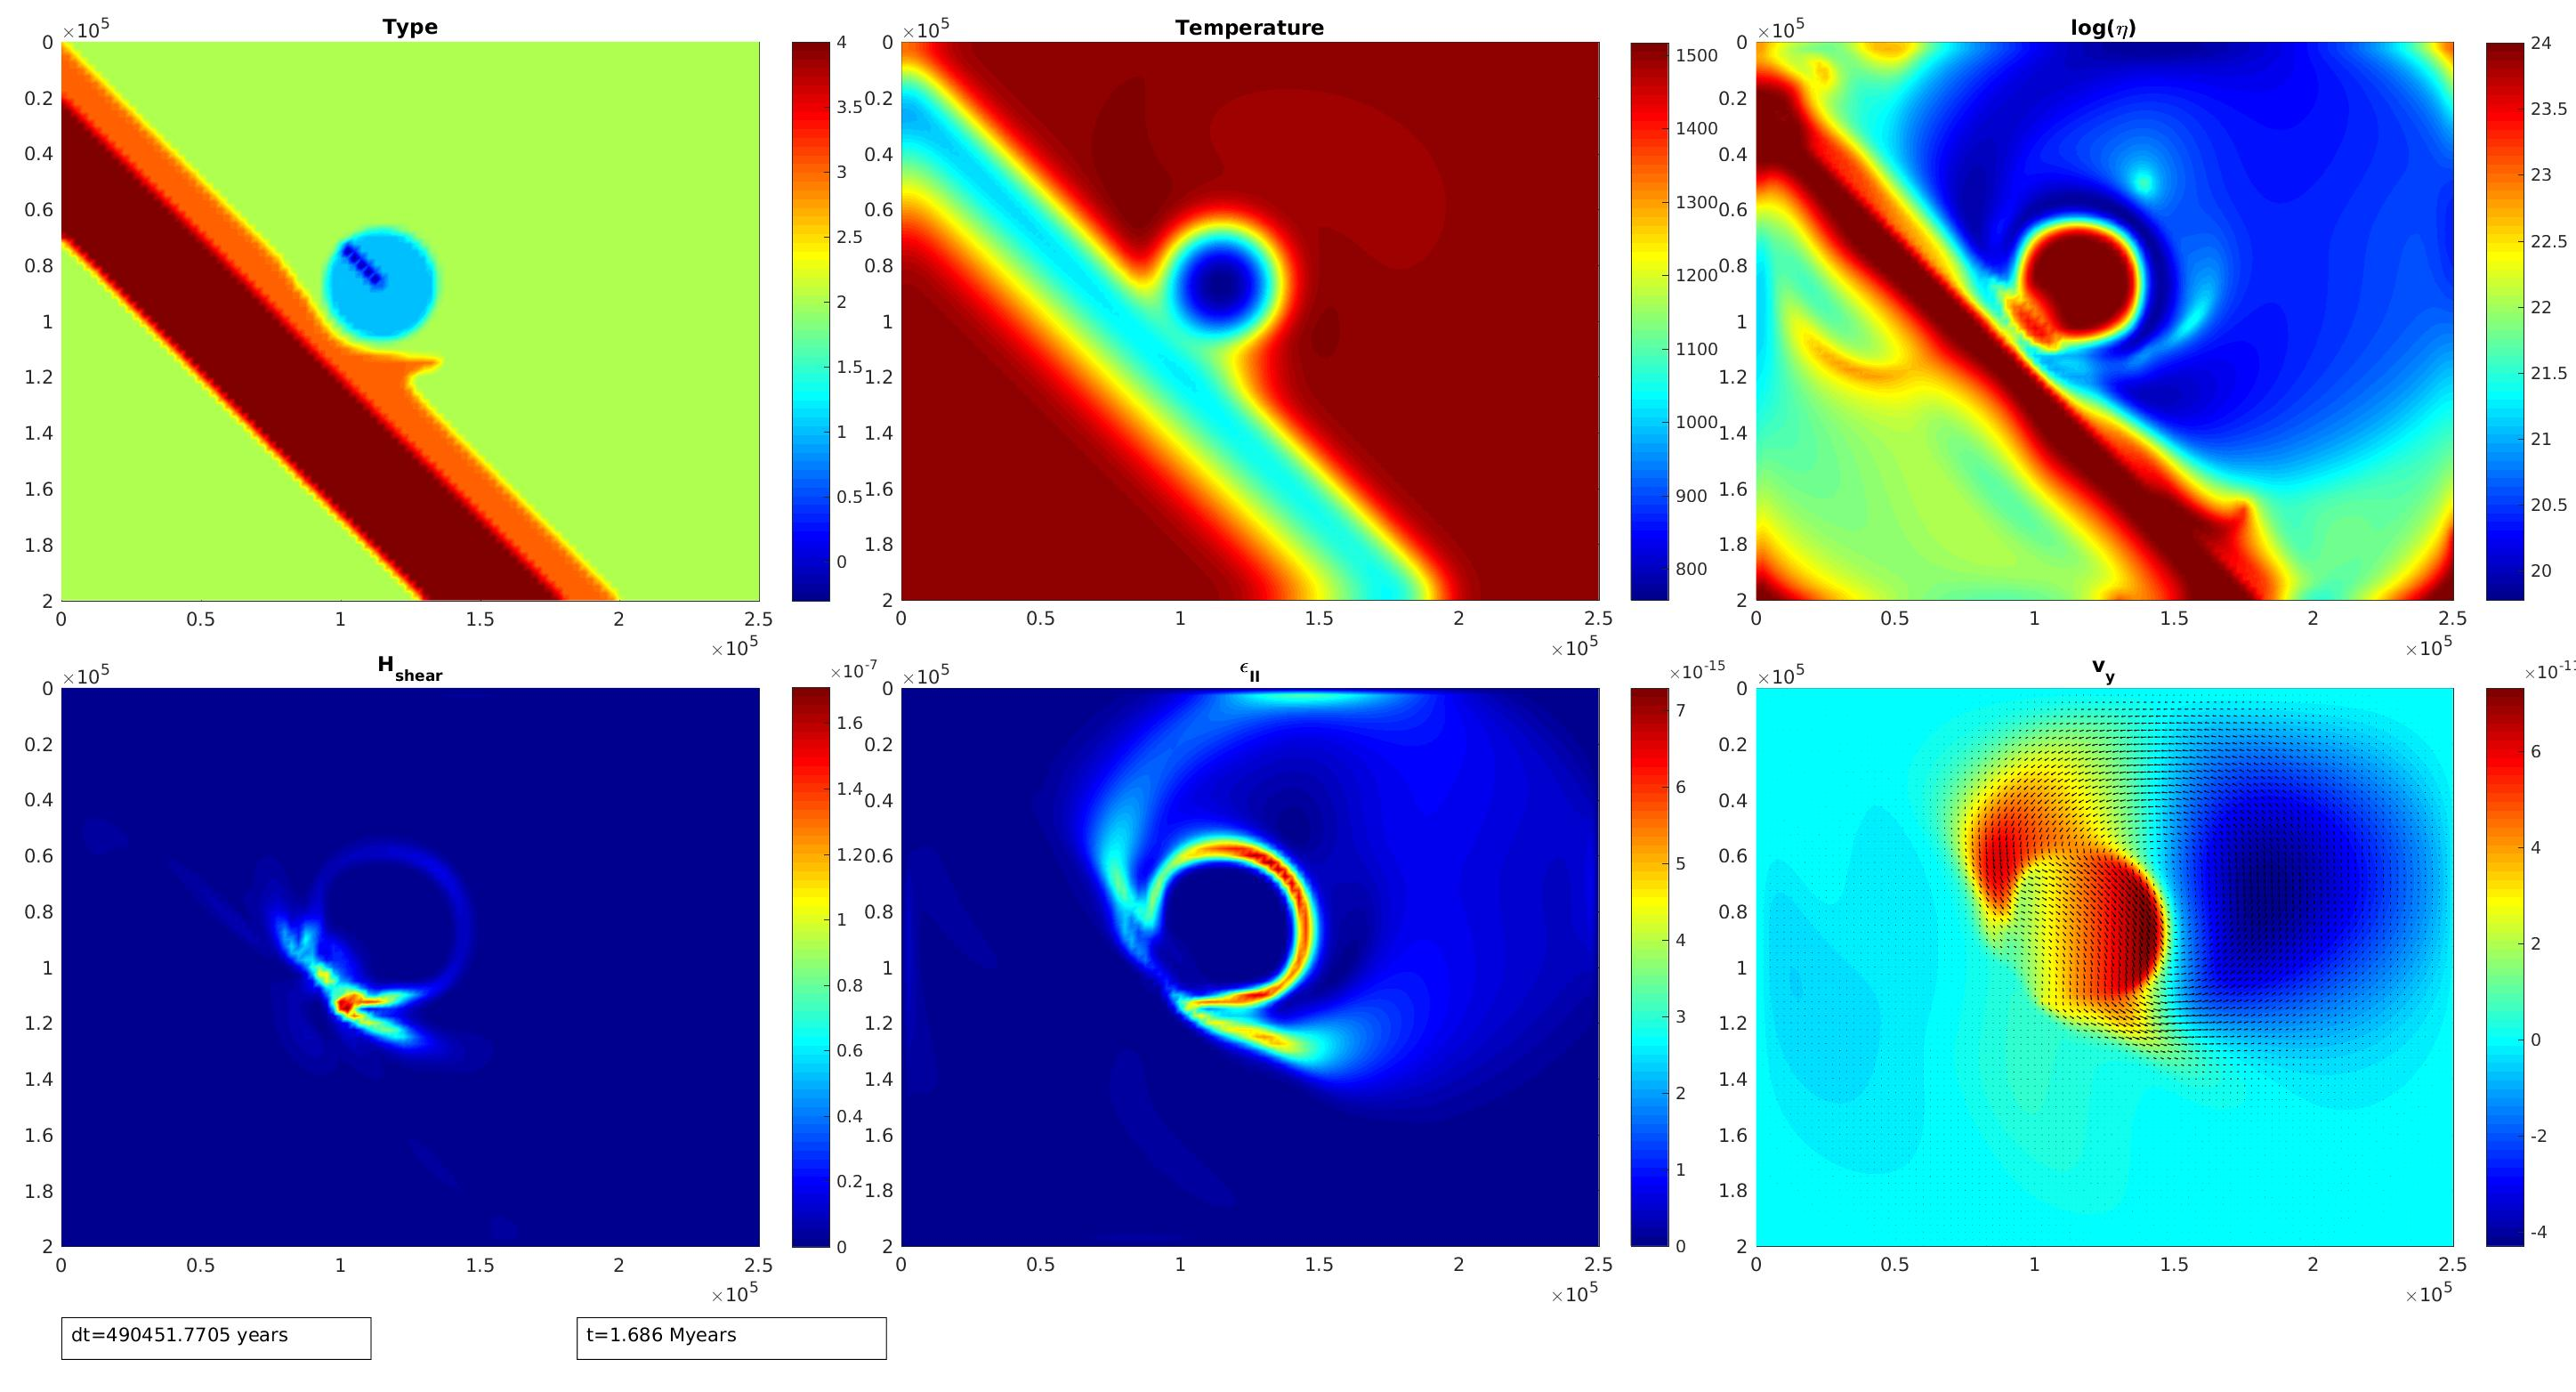
\includegraphics[width=1.0\textwidth]{./Snapshots/bulldozer/posleft45/Subductionzonewithblob72posleftslab45s5e7s1e7r20.jpg}
		\end{minipage}
		\begin{minipage}[t]{0.5\textwidth}
			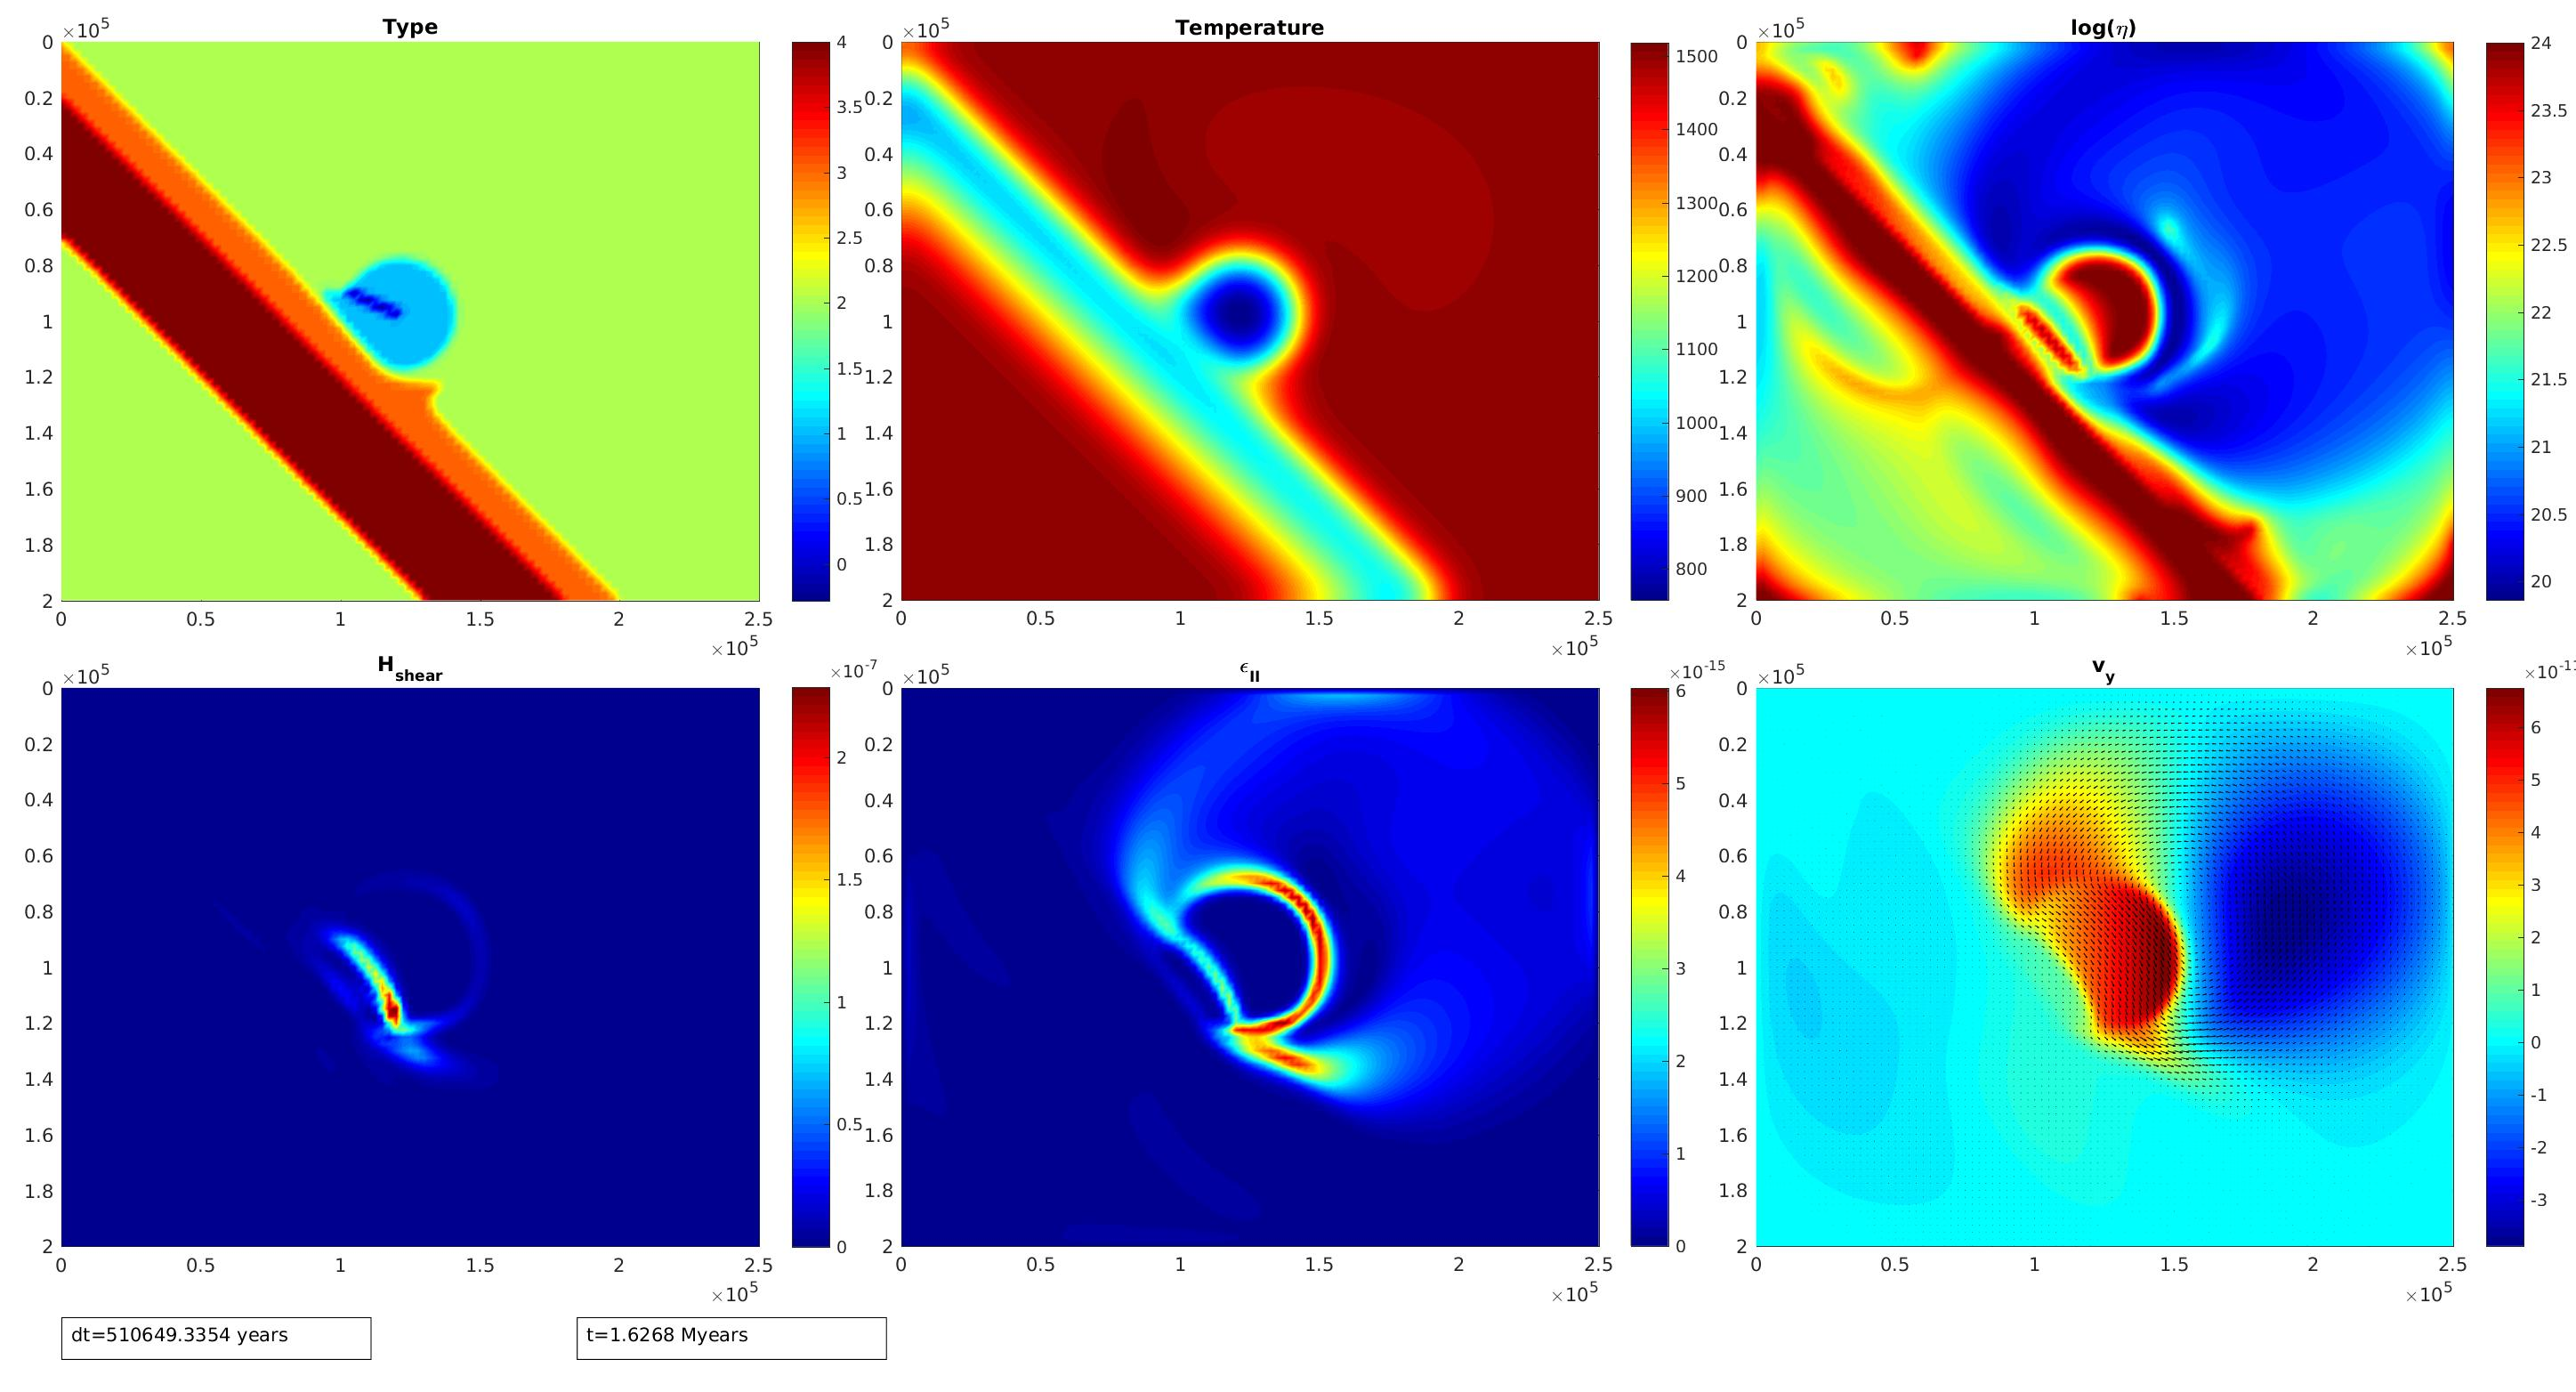
\includegraphics[width=1.0\textwidth]{./Snapshots/bulldozer/posleft45/Subductionzonewithblob81posleftslab45s2e7s1e7r20.jpg}
		\end{minipage}
	\end{minipage}
	\caption{State around 2 million years with varying strengths}
	\label{fig:bulldozer45}
\end{figure}
The goal was to maximize the visible bulldozer effect in a 2 million year timeframe where the shape should remain similar to the data. This was done by simulating the 30 degrees angle model with varying all other parameters. The following observations were made. When the radius of the plume exceeded 20 kilometers it was no longer feasible to get this bulldozer effect in the mentioned timeframe. The bigger the plume the more time was needed for the model to resemble the shape of the data. Therefore only radii of 10-20 kilometers were used for the follow up simulations. Further was observed that when the fraction of the strengths is smaller than $50$, meaning cases where the strengths for plume and plate were not $10^8/10^6$, $5\cdot 10^7/10^6$ or $10^8/2\cdot 10^6$, the diameter of the pushed material was to small compared to the actual data. Additionally it was noted that the distance between plume and plate should be close to the contact point. This was not surprising since it was already known that the plume will never collide with the plate at maximum velocity since the material in front of the plume always decelerate the plume itself massively. Furthermore this material in front depending on the strength of the plate can already "dig" into the plate before the plume arrives. A good match chosen from 12 simulations is shown in figure \ref{fig:goodmatch1} and \ref{fig:goodmatch2}.

\begin{figure}[!ht]
\begin{minipage}[t]{1.0\textwidth}
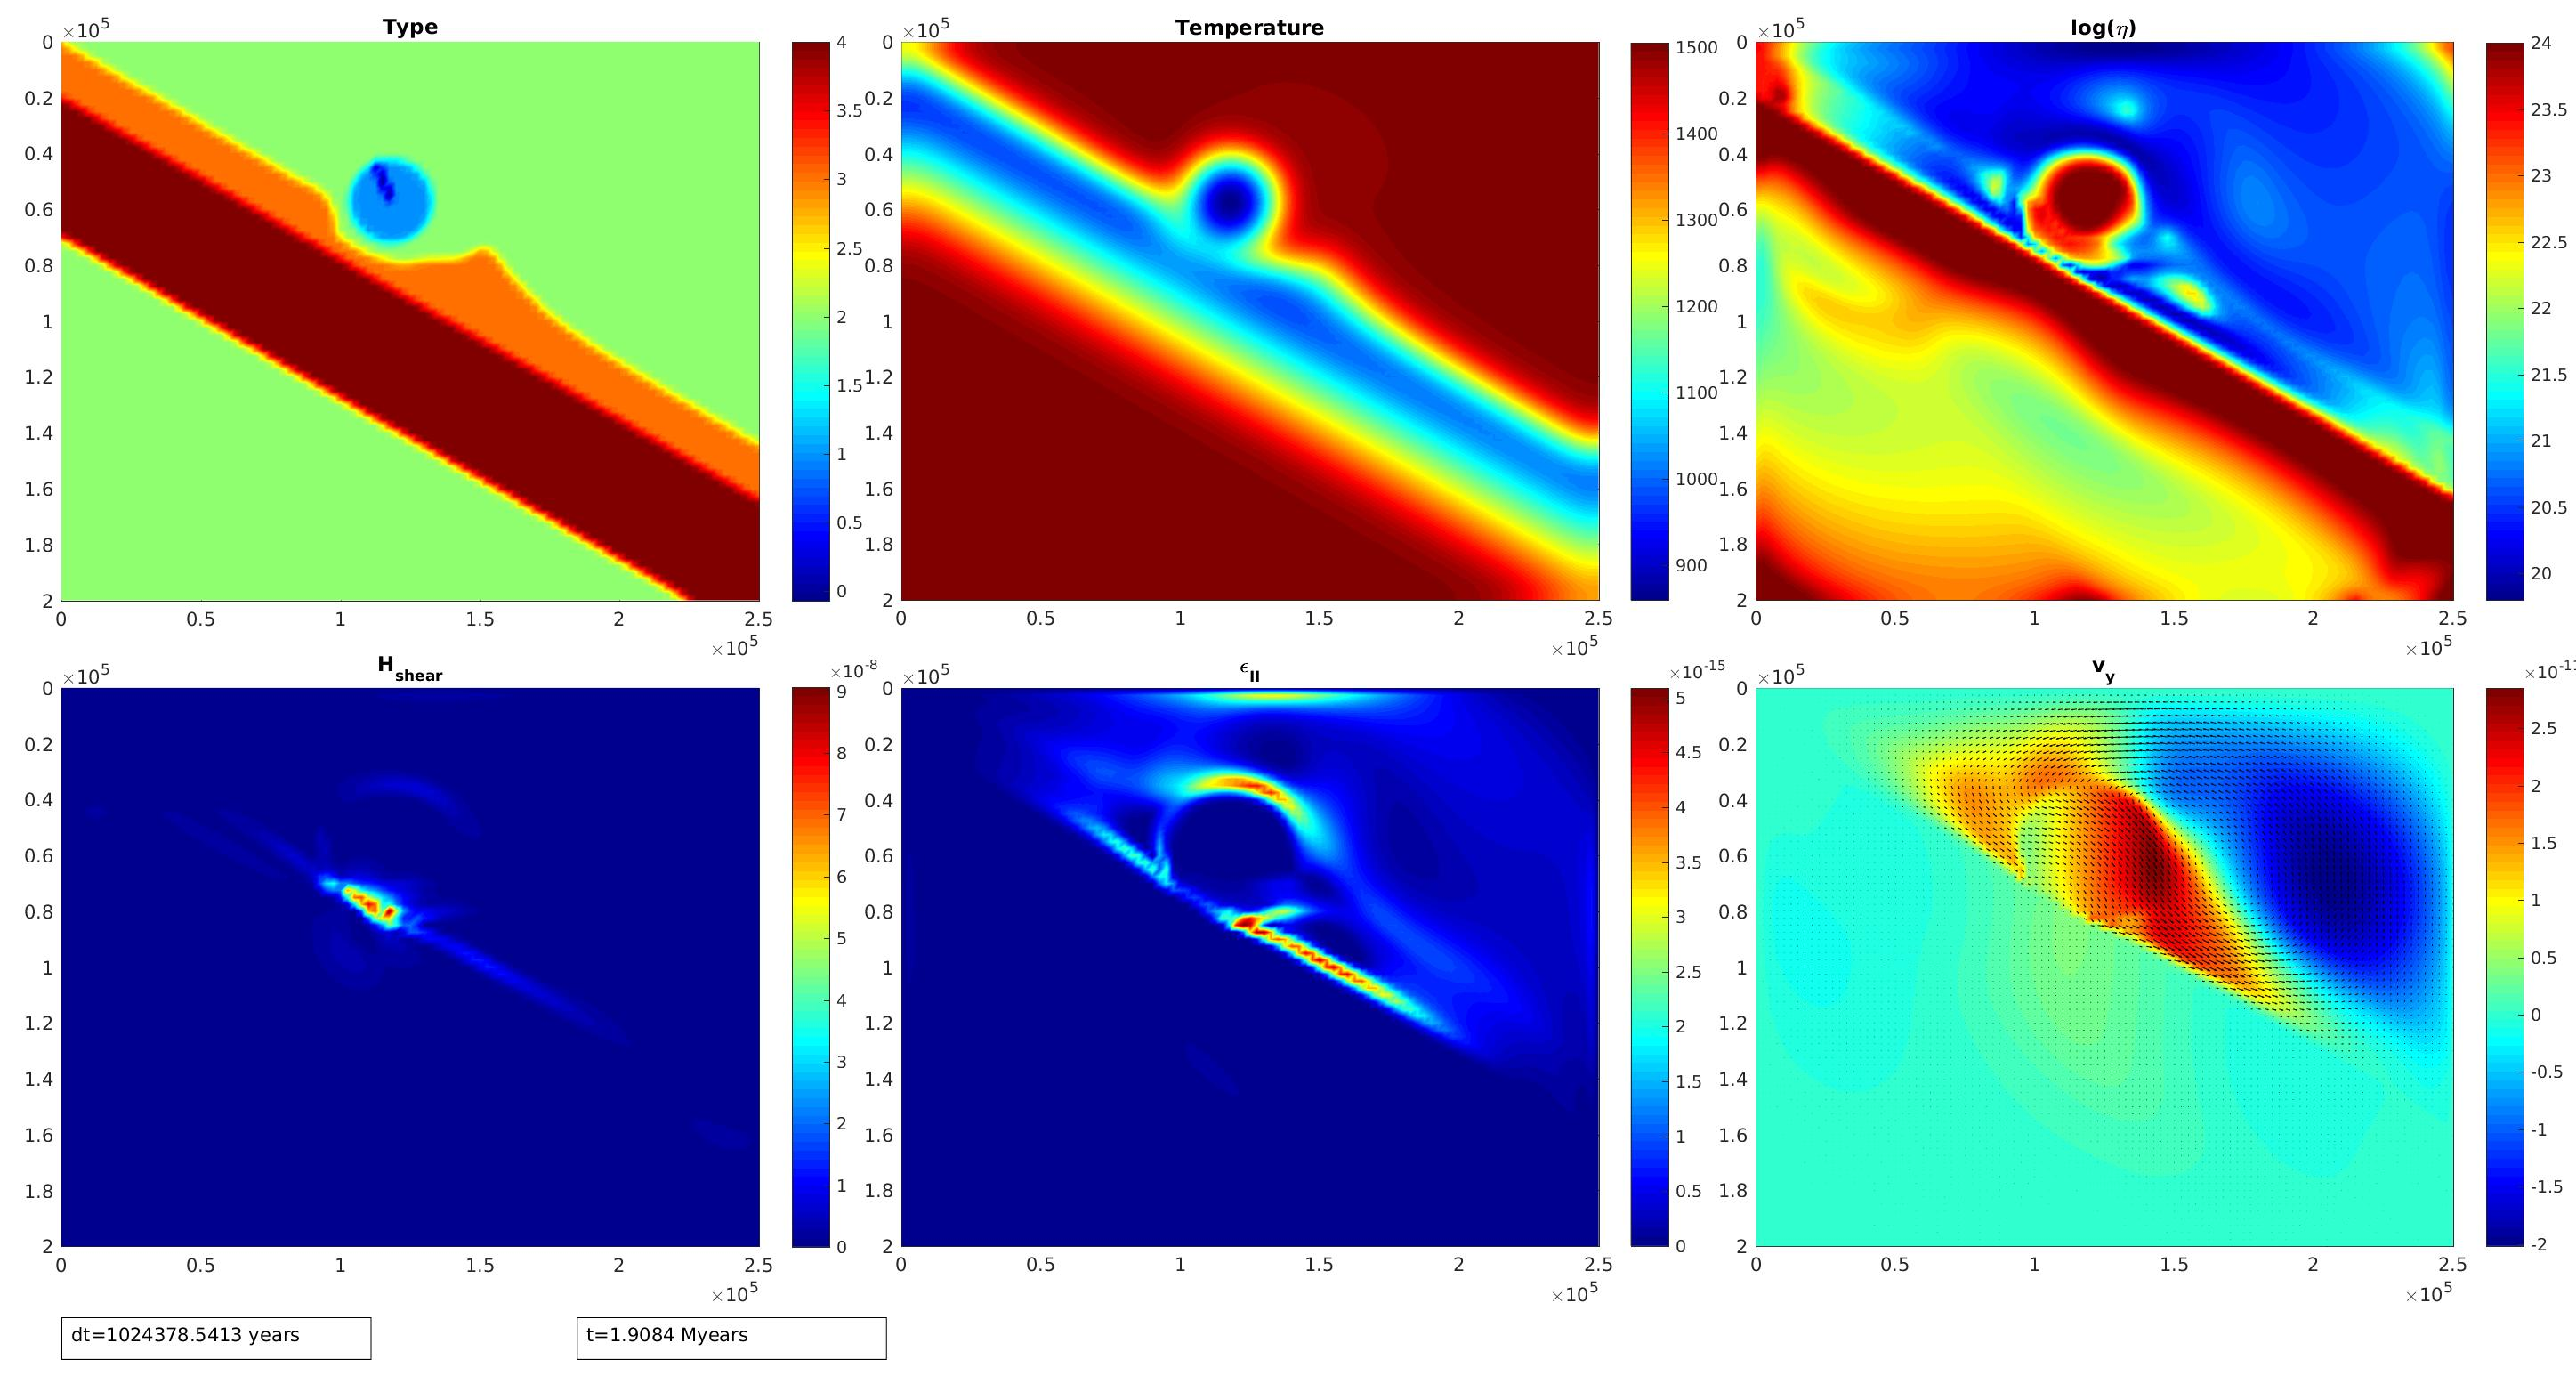
\includegraphics[width=1.0\textwidth]{./Snapshots/bulldozer/posleft30/Subductionzonewithblob38posleft3slab30s5e7s1e6r15.jpg}
\end{minipage}
\caption{shortly before 2 million years in 30 degrees case with 15 kilometer radius und $5 \cdot10^7/10^6$ strength}
\label{fig:goodmatch1}
\end{figure}

\begin{figure}[!ht]
\begin{minipage}[t]{1.0\textwidth}
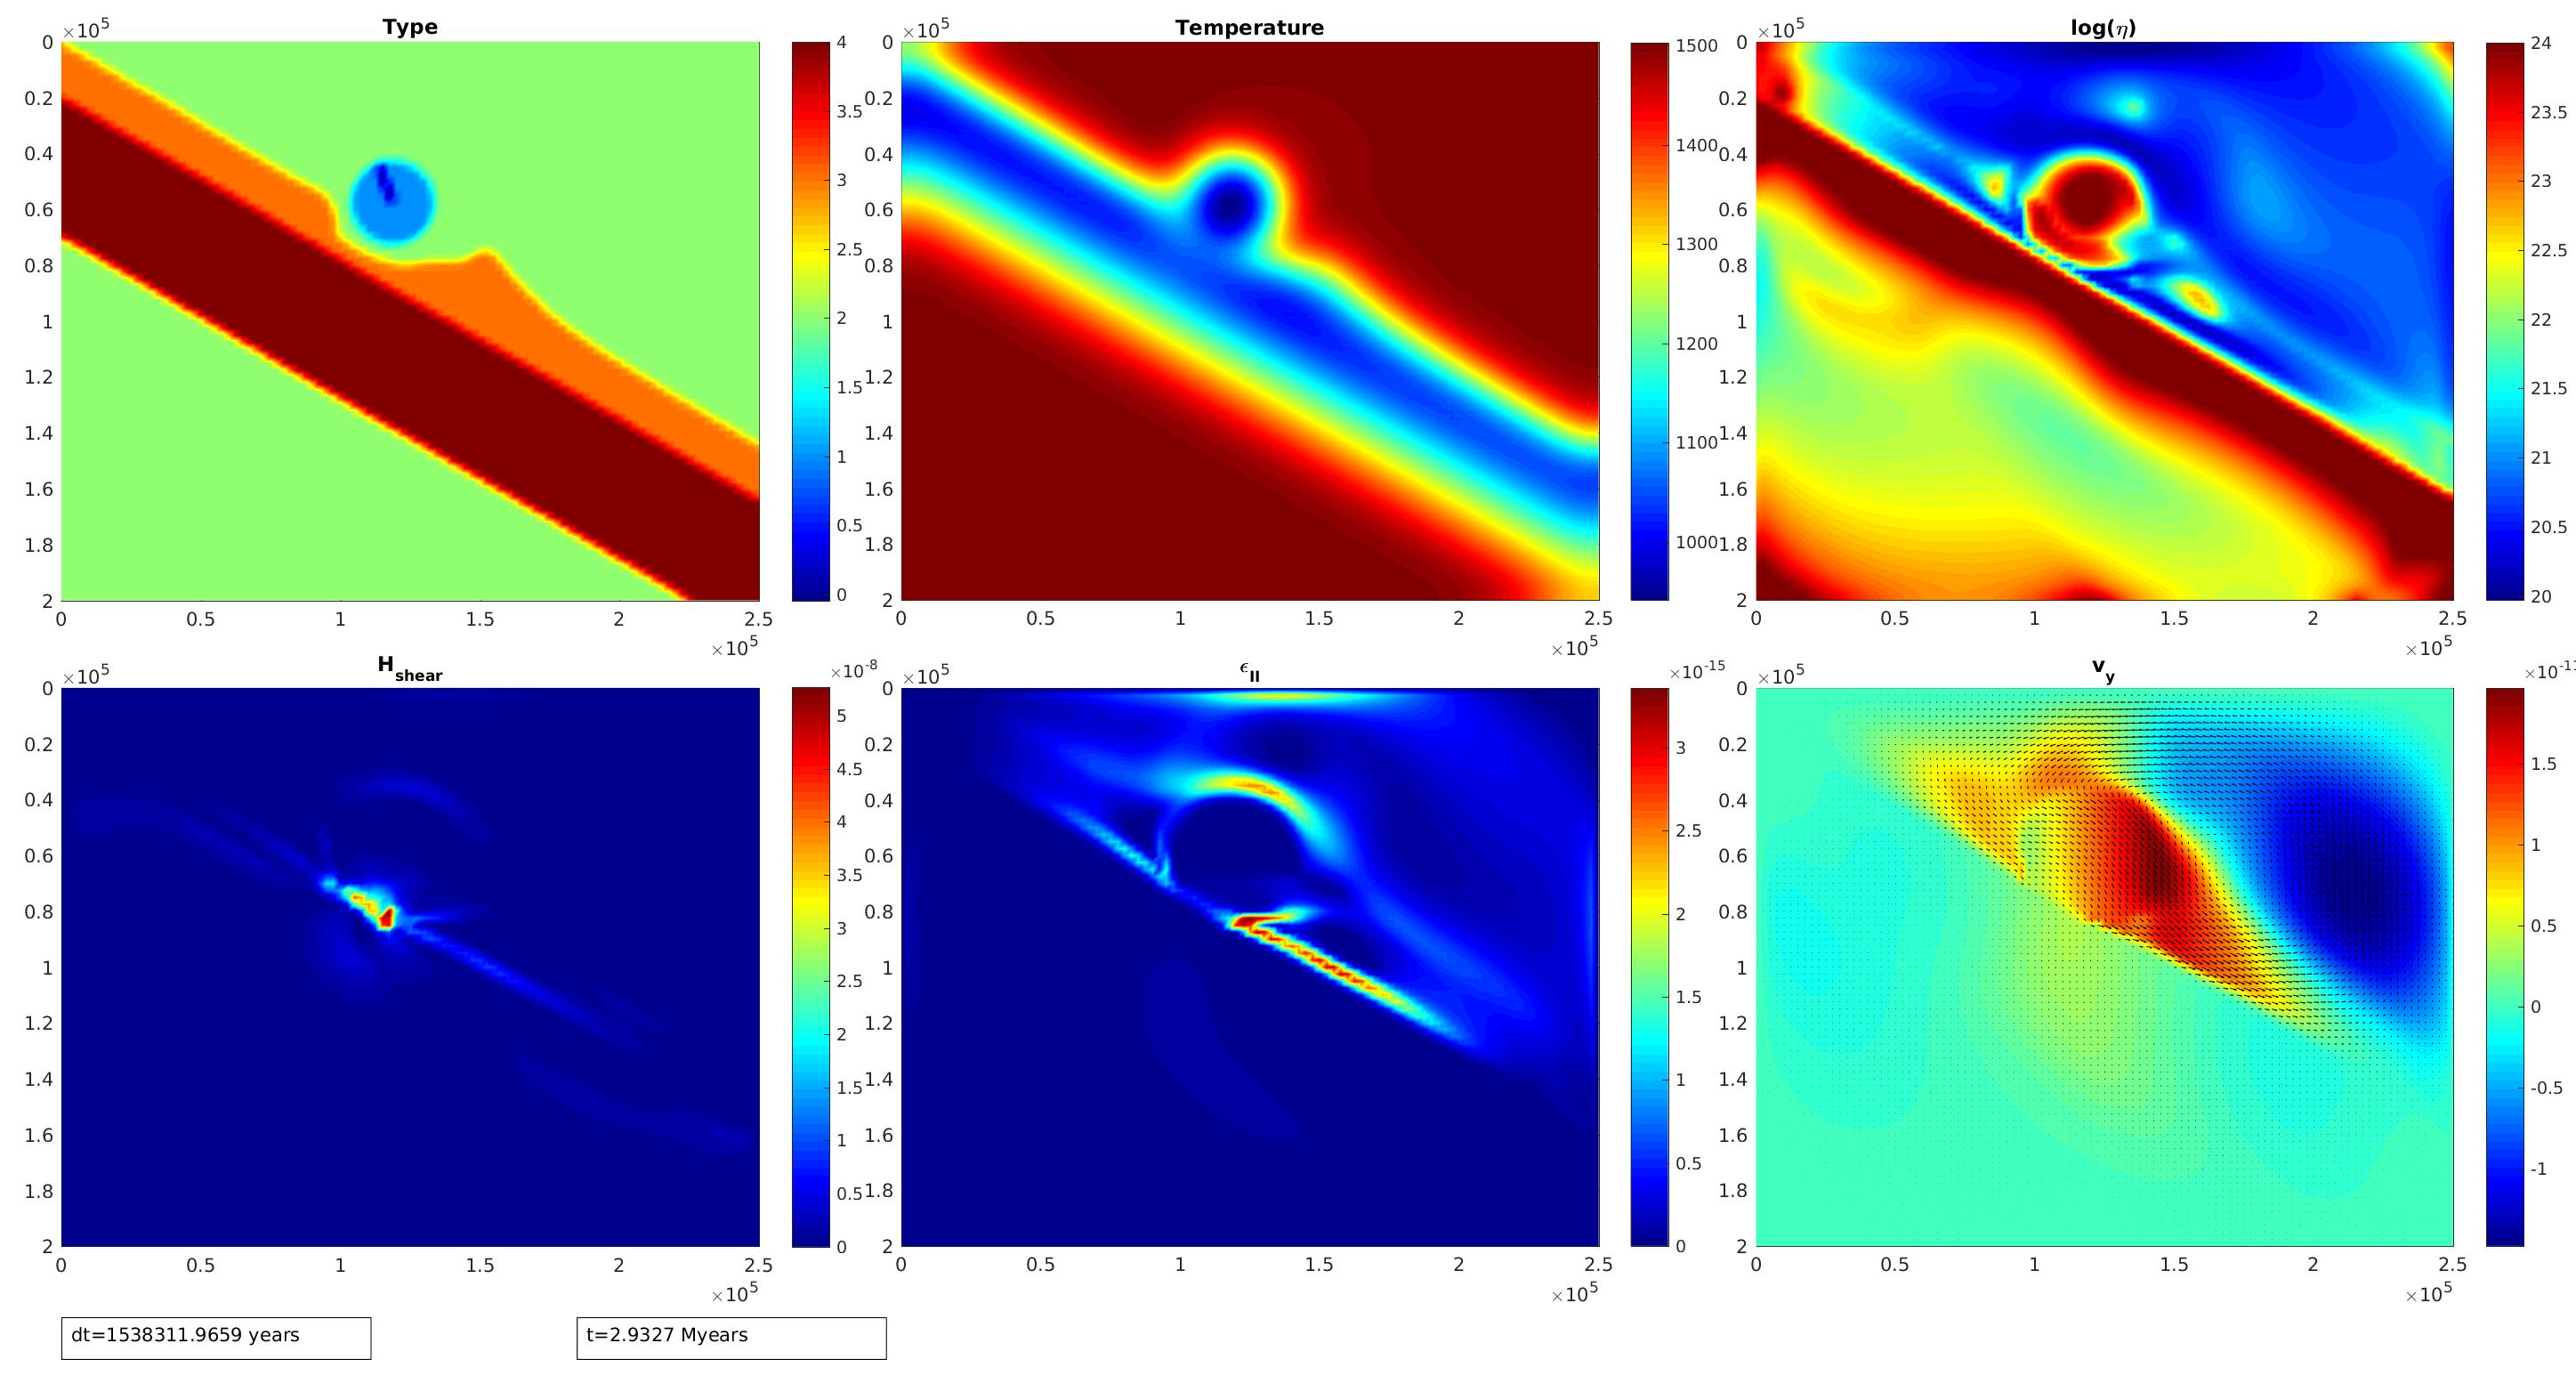
\includegraphics[width=1.0\textwidth]{./Snapshots/bulldozer/posleft30/Subductionzonewithblob39posleft3slab30s5e7s1e6r15.jpg}
\end{minipage}
\caption{shortly after 2 million years in 30 degrees case with 15 kilometer radius und $5 \cdot10^7/10^6$ strength}
\label{fig:goodmatch2}
\end{figure}

\subsection{Late stage development}
One could observe two overall tendencies. The first one is in case where the strength of both plate and plume are nearly equal furthermore the angle is over 45 degrees. In this scenario the plume will be deflected by the plate and will slowly slider over the edge without disrupting the overall structure. In the second case the main difference is the strength of the plume is significant higher than the plate. This could lead to different scenarios. One is that only the buffer zone on the plate will be disrupted and the plume will still slide over the plate like the bulldozer effect described. A second one is that in case of a flat angle, 20 or 30 degrees, and small radii, 10-20 kilometers, the plume could cut through the plate over long timescales. Due to the limitation of the model a third interesting longterm tendency could not be produced. This would be with high probability the case where there is a flat angle and big radius leads to the tendency where the plume helps the plate to brake of at the necking area and sinks together with the plate into the asthenosphere. Overall also a longterm tendency of the temperature field could also not be produced because of the limitation in numerical diffusion.

\section{Conclusion}
In conclusion one cannot underestimate the complexity of a model although it was strongly reduced. Although the reduced model had small degrees of freedom left(limited fixed values) in comparison to the full model the actual number of scenarios which could develop is still astonishingly high inclusive the unphysical cases. Although a numerical simulation has number of limitations and one has to be careful, since solving a partial differential equation numerically is in most cases not easy, it still can help to give insights to understand the problem better and possibly improve the existing models, in this case in geophysics where also rare events exist, and also to have a possible outlook for the future how the situation can develop.

\nocite{vargas2013tearing}
\nocite{gerya2009introduction}




\newpage

\bibliographystyle{plain}
\bibliography{references}


\end{document}

